\chapter{Metodologias propostas}\label{chap3}

Esse capítulo propõe três metodologias para avaliação de incerteza em modelos geológicos multi-categóricos usando funções distâncias assinaladas. Todos os métodos são acompanhados de uma prova de conceito no banco de dados \textit{Swiss Jura} e um estudo de caso. 

\section{Parametrização do suporte do \textit{kernel}}

Esse método é uma adaptação do condicionamento das amostras apresentado no \autoref{chap:cond_amo}, para que além de poder ser aplicado para múltiplos domínios, seja mais versátil. No método proposto por \citeonline{mclennanstationarity} o interpolador fica restrito ao inverso do quadrado já que outros interpoladores podem gerar pesos negativos que interferem na ponderação gerada pelo condicionamento das amostras.

A adaptação propõe, no lugar de modificar o peso dado às amostras, modificar o suporte dos \textit{kernels} usados na interpolação por funções de bases radiais multiplicando-os por um fator menor (pessimista) ou maior (otimista) que um. Para cada categoria do depósito mineral, os cenários otimistas, pessimista e caso base são gerados e combinados para criar múltiplos cenários para o modelo geológico multi-categórico.

Considere o exemplo em uma dimensão da \autoref{one_dim_ex}. A figura mostra quatro amostras, duas azuis que não pertencem ao domínio sendo modelado, e duas vermelhas que pertencem ao domínio sendo modelado. As amostras estão, da esquerda para a direita, nas posições 1, 10, 70 e 90.

\begin{figure}[H]
	\caption{\label{one_dim_ex} Amostras em posição 1, 10, 70 e 90. Amostras em azul não pertencem ao domínio enquanto amostras vermelhas pertencem.}
	\centering
		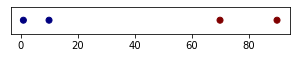
\includegraphics[width=0.4\textwidth]{capitulo_3/imagens/pointssd.png}
\end{figure}

A \autoref{uni_rbf} mostra, no gráfico horizontal abaixo as amostras da \autoref{one_dim_ex} e no eixo y do gráfico o valor da função distância assinalada calculada para cada uma das quatro amostras. A Figura \autoref{at} uma função RBF com suporte igual a 25 centrada em cada uma das amostras. A Figura \autoref{dt} mostra, em preto, a superfície interpolada a partir da combinação das quatro RBFs após o cálculo dos pesos a partir do sistema de equações apresentado na \autoref{rbf_sist}. O limite do domínio é onde a distância assinalada interpolada é igual a zero.

\begin{figure}[H] 
    \centering
    \caption{Exemplo em uma dimensão no gráfico abaixo e distâncias assinaladas calculadas para cada uma das amostras no eixo y.} \label{uni_rbf}
     \subfloat[][Uma RBF com suporte igual a 25 e centrada em cada uma das amostas.]{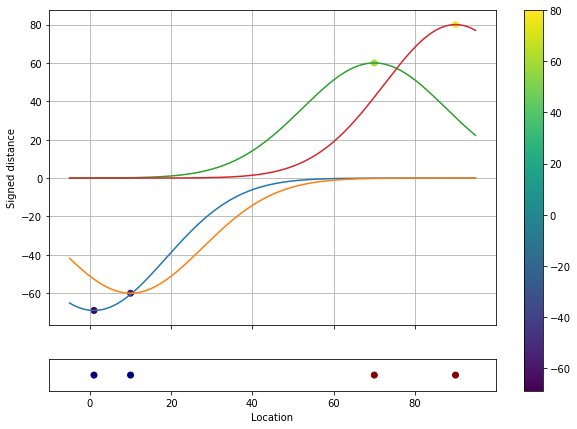
\includegraphics[width=.45\textwidth]{capitulo_3/imagens/RBF_before_train.png}\label{at}}
     \hspace{1em}
     \subfloat[][Uma RBF com suporte igual a 25 e centrada em cada uma das amostas após o cálculo dos pesos e sua combinação linear em preto.]{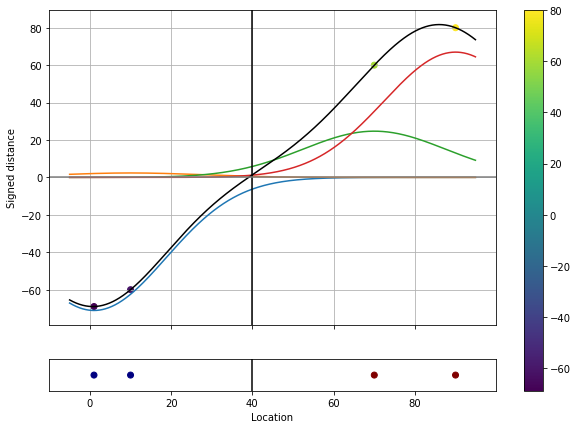
\includegraphics[width=.45\textwidth]{capitulo_3/imagens/RBF_after_train.png}\label{dt}}
\end{figure}

O método proposto modifica o suporte de uma cada uma das RBFs centradas nas amostras de acordo com o valor da distância assinalada calculada para aquela amostras a partir das curvas de parametrização mostradas na \autoref{param}. Dessa forma, cada RBF terá um suporte diferente. O volume do sólido gerado pelo cenário otimista é maior do que o gerado pelo caso baso enquanto o volume do sólido gerado pelo caso pessimista é menor.

\begin{figure}[H] 
    \centering
    \caption{Parametrização das amostras.} \label{param}
     \subfloat[][Linear.]{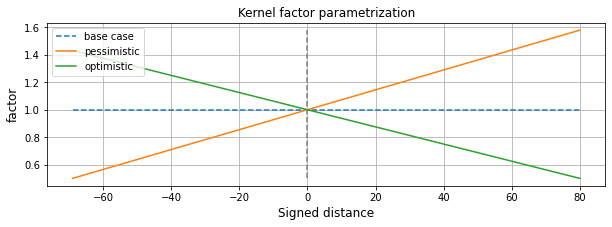
\includegraphics[width=.8\textwidth]{capitulo_3/imagens/linear_kfp.png}\label{paramlinear}} \\
     \subfloat[][Quadrática.]{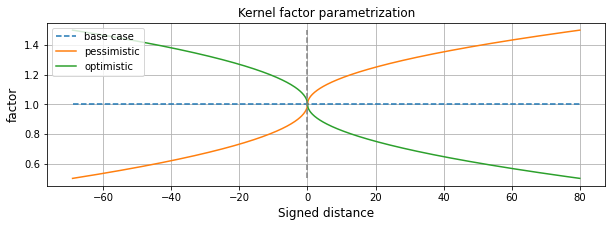
\includegraphics[width=.8\textwidth]{capitulo_3/imagens/quadratic_kfp.png}\label{paramquadrat}}
\end{figure}

A \autoref{dif_kernel} mostra as RBFs, que na \autoref{uni_rbf} tinham suporte igual a 25, com seus suportes modificados a partir das curvas de parametrização lineares mostradas na Figura \autoref{paramlinear}. Os pesos são então calculados para cada um dos casos e uma superfície interpolada pode ser gerada a partir da combinação linear das RBFs.

\begin{figure}[H] 
    \centering
    \caption{Exemplo em uma dimensão no gráfico abaixo e distâncias assinaladas calculadas para cada uma das amostras no eixo y.} \label{dif_kernel}
     \subfloat[][Caso otimista.]{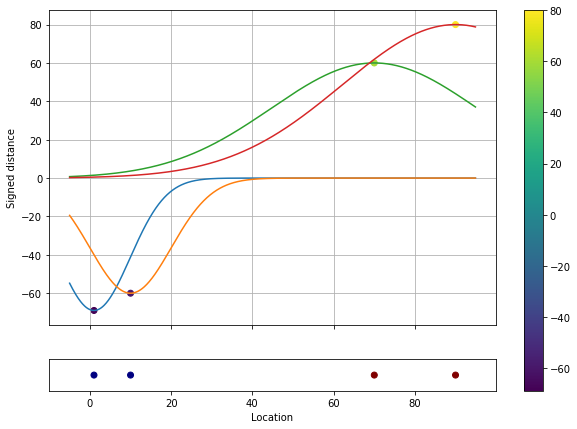
\includegraphics[width=.45\textwidth]{capitulo_3/imagens/pessimistic_kernels.png}\label{<figure1>}}
     \hspace{1em}
     \subfloat[][Caso pessimista.]{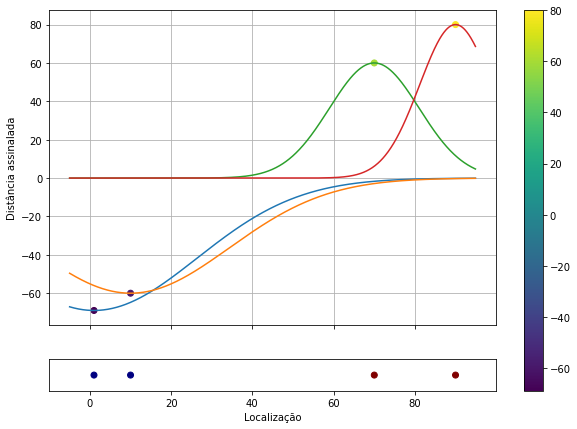
\includegraphics[width=.45\textwidth]{capitulo_3/imagens/optmistic_kernels.png}\label{<figure2>}}
\end{figure}

A \autoref{one_dim_result} mostra, em preto, a superfície interpolada para o caso base, em vermelho, para o cenário pessimista e em azul para o cenário otimista. 
 
\begin{figure}[H]
	\caption{\label{one_dim_result} Caso base e cenários otimista e pessimista para o exemplo unidimensional proposto.}
	\centering
		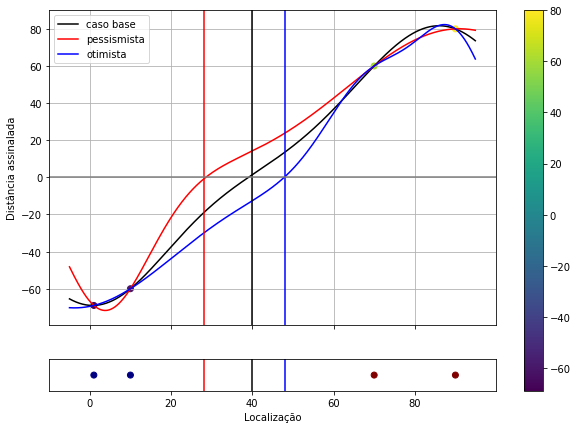
\includegraphics[width=0.6\textwidth]{capitulo_3/imagens/all_kernels.png}
\end{figure}

A aplicação do método no banco de dados \textit{Swiss Jura} consiste em, calcular as distâncias assinaladas para cada uma das cinco categorias do banco de dados. Então os parâmetros para modificação do suporte devem ser escolhidos. Nesse caso, um modelo linear com valor de f mínimo igual a 0.95. A \autoref{quater_param} mostra as distâncias assinaladas para a categoria Quaternary interpoladas para o cenário pessimista, caso base e cenário otimista. Os mesmos cenários foram interpolados para as outras quatro categorias do banco de dados.

\begin{figure}[H] 
    \centering
    \caption{Distâncias assinaladas interpoladas para a categoria Quaternary do banco de dados \textit{Jura} para o caso base, e cenários pessimista e otimista.} \label{quater_param}
     \subfloat[][Caso pessimista.]{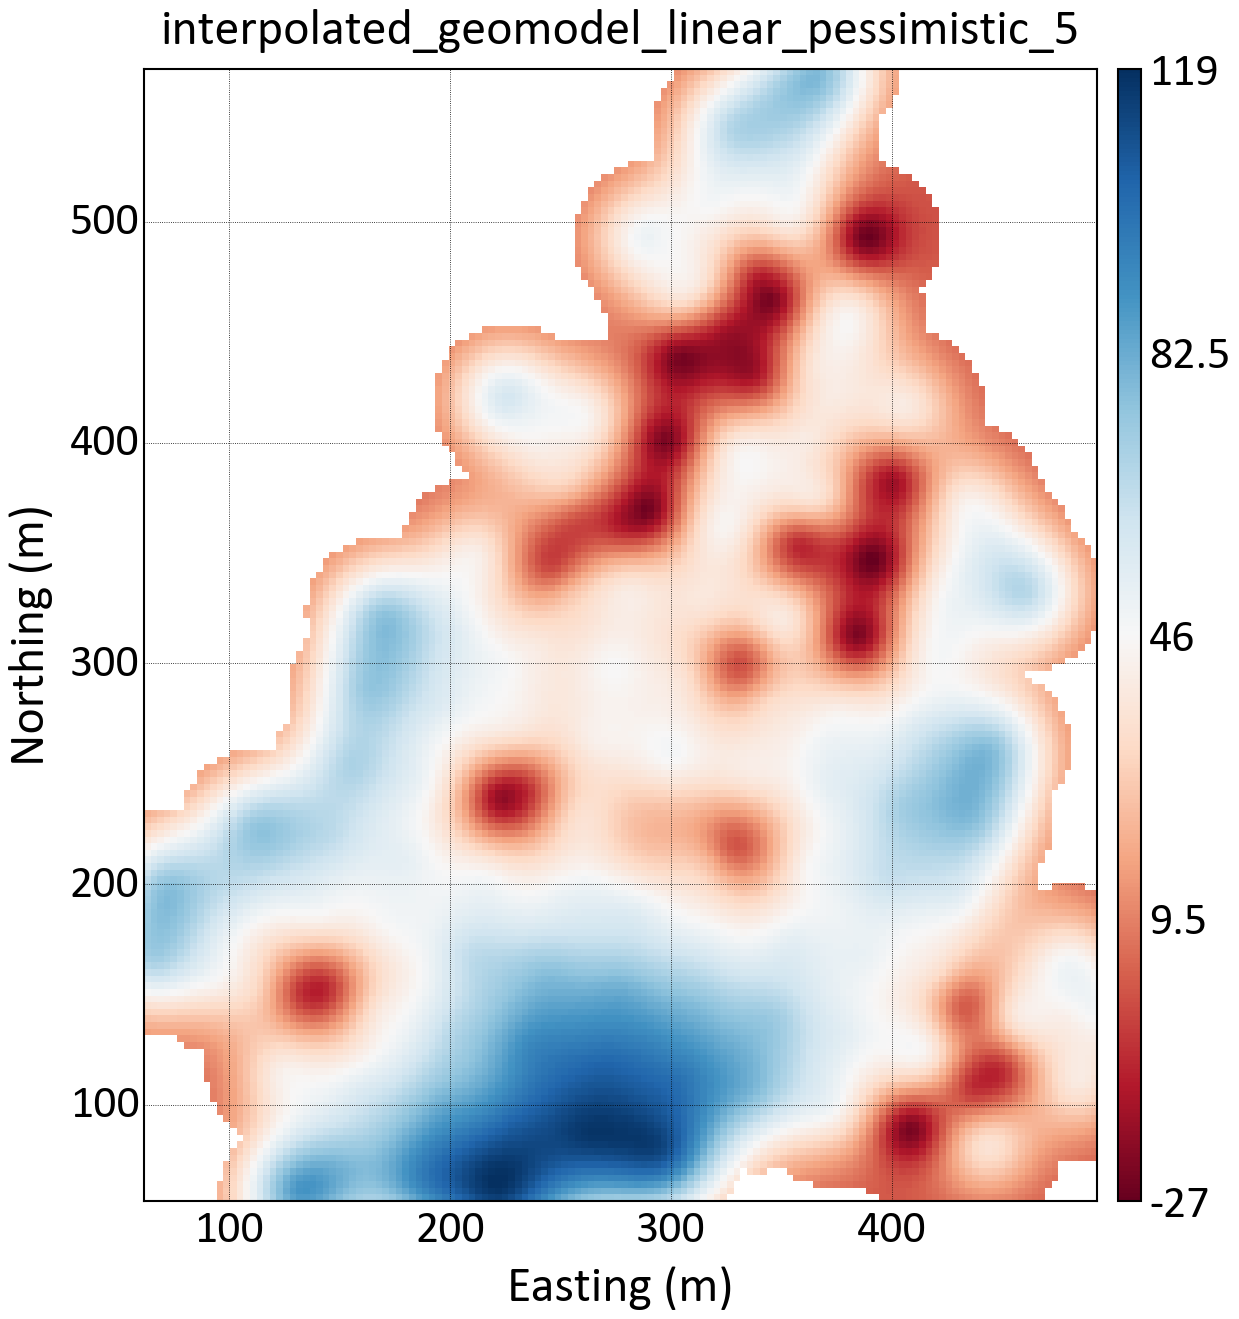
\includegraphics[width=.3\textwidth]{capitulo_3/imagens/pessimistic.png}\label{<figure1>}}
     \hspace{1em}
     \subfloat[][Caso base.]{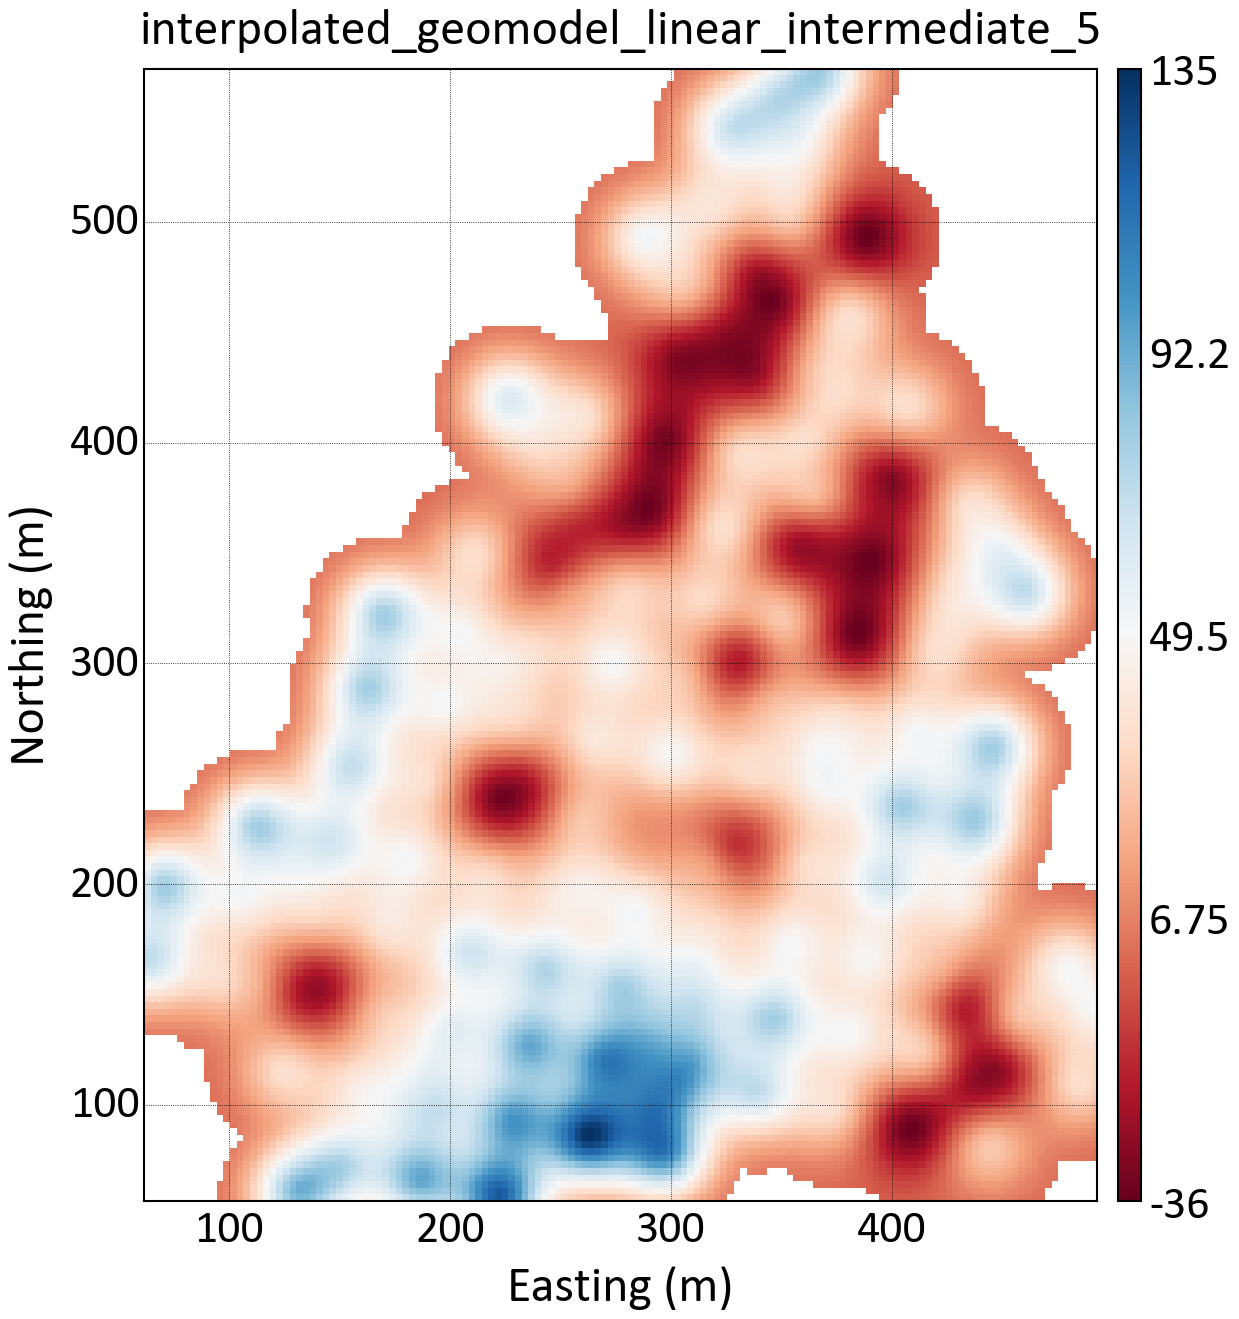
\includegraphics[width=.3\textwidth]{capitulo_3/imagens/intermediate.png}\label{<figure2>}}
     \hspace{1em}
     \subfloat[][Caso otimista.]{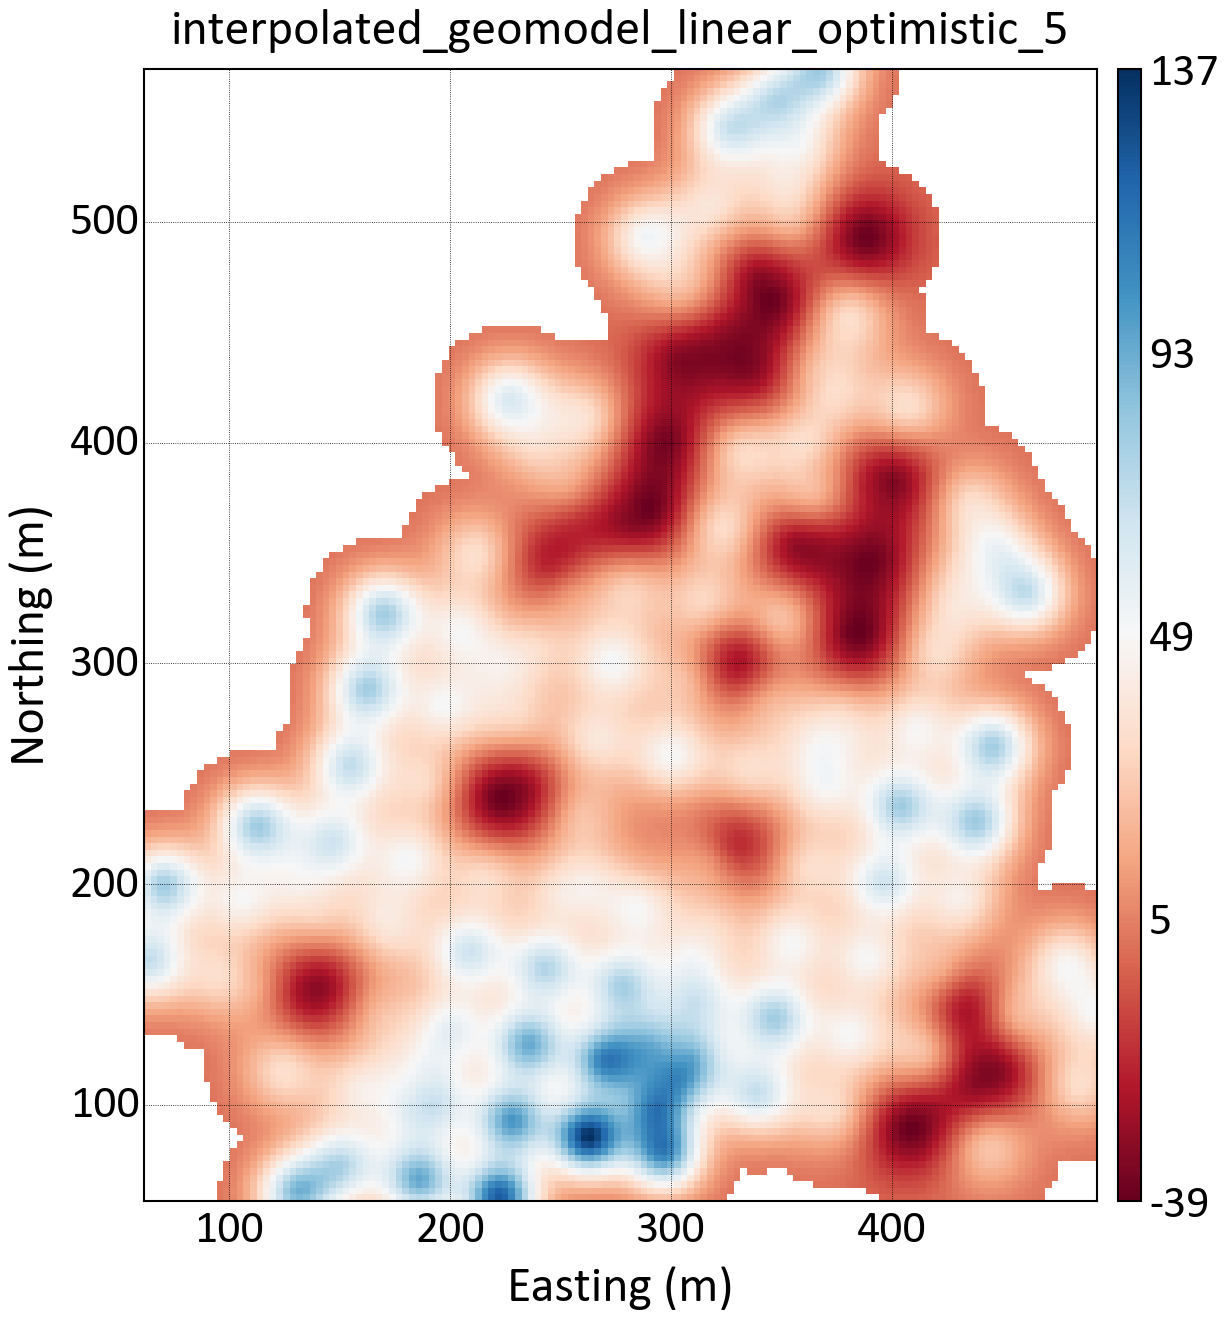
\includegraphics[width=.3\textwidth]{capitulo_3/imagens/optimistic.png}\label{<figure3>}}
\end{figure}

Para cada categoria há três diferentes cenários que devem ser combinados para criar os modelos geológicos multi-categóricos. Em alguns casos, a combinação do cenário otimista de uma categoria com grande área ou grande volume com o cenário pessimista de uma categoria de pequena área ou volume pode fazer com nenhum bloco seja atribuído à menor categoria em alguns dos $3^K$ modelos. Onde K é o número de categorias do banco de dados.  

Para contornar esse problema os modelos devem passar por um teste de reprodução dos dados amostrais. O algoritmo checa se o bloco com o centroide mais próximo a cada amostra foi classificado com a mesma categoria daquela amostra. O usuário seleciona um nível mínimo de reprodução, nesse caso 0.9. Desse modo, modelos que não reproduzem, pelo menos, 90\% dos dados amostrais são descartados. Dos 243 modelos gerados para o \textit{Swiss Jura} combinando os três cenários para as cinco diferentes categorias, 24 não foram descartados já que reproduzem, pelo menos, 90\% das amostras. 

A \autoref{jura_kernel} mostra duas realizações escolhidas aleatoriamente entre as 24 selecionadas, juntamente com as amostras representadas pelos círculos. Uma animação mostrando todas elas pode ser vista \href{https://github.com/robertorolo/kernel_support_parametrization_uncertainty_assess/blob/main/ezgif-7-b96e150c9939.gif}{aqui}.

\begin{figure}[H] 
    \centering
    \caption{Modelos geológicos para o \textit{Swiss Jura} criados a partir da parametrização do suporte do \textit{kernel}.} \label{jura_kernel}
     \subfloat[][Modelo 200.]{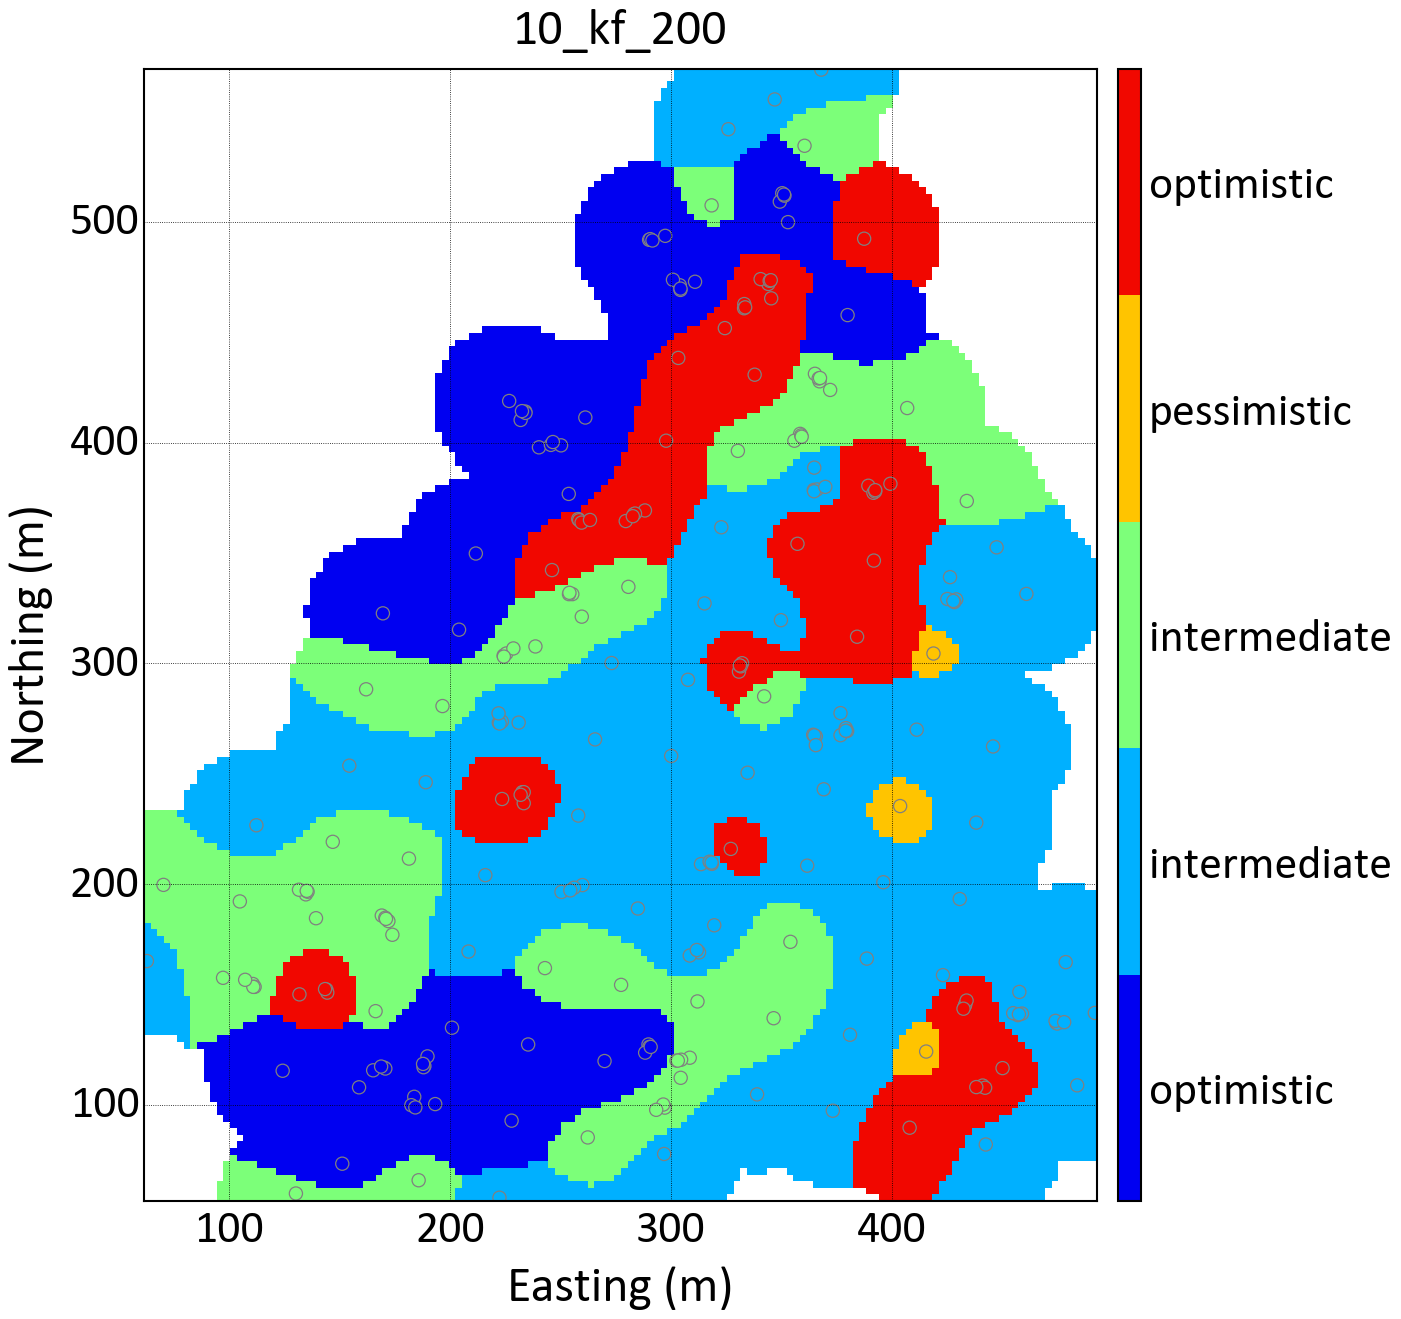
\includegraphics[width=.45\textwidth]{capitulo_3/imagens/out_model_10_kf_200.png}\label{<figure1>}}
     \hspace{1em}
     \subfloat[][Modelo 214.]{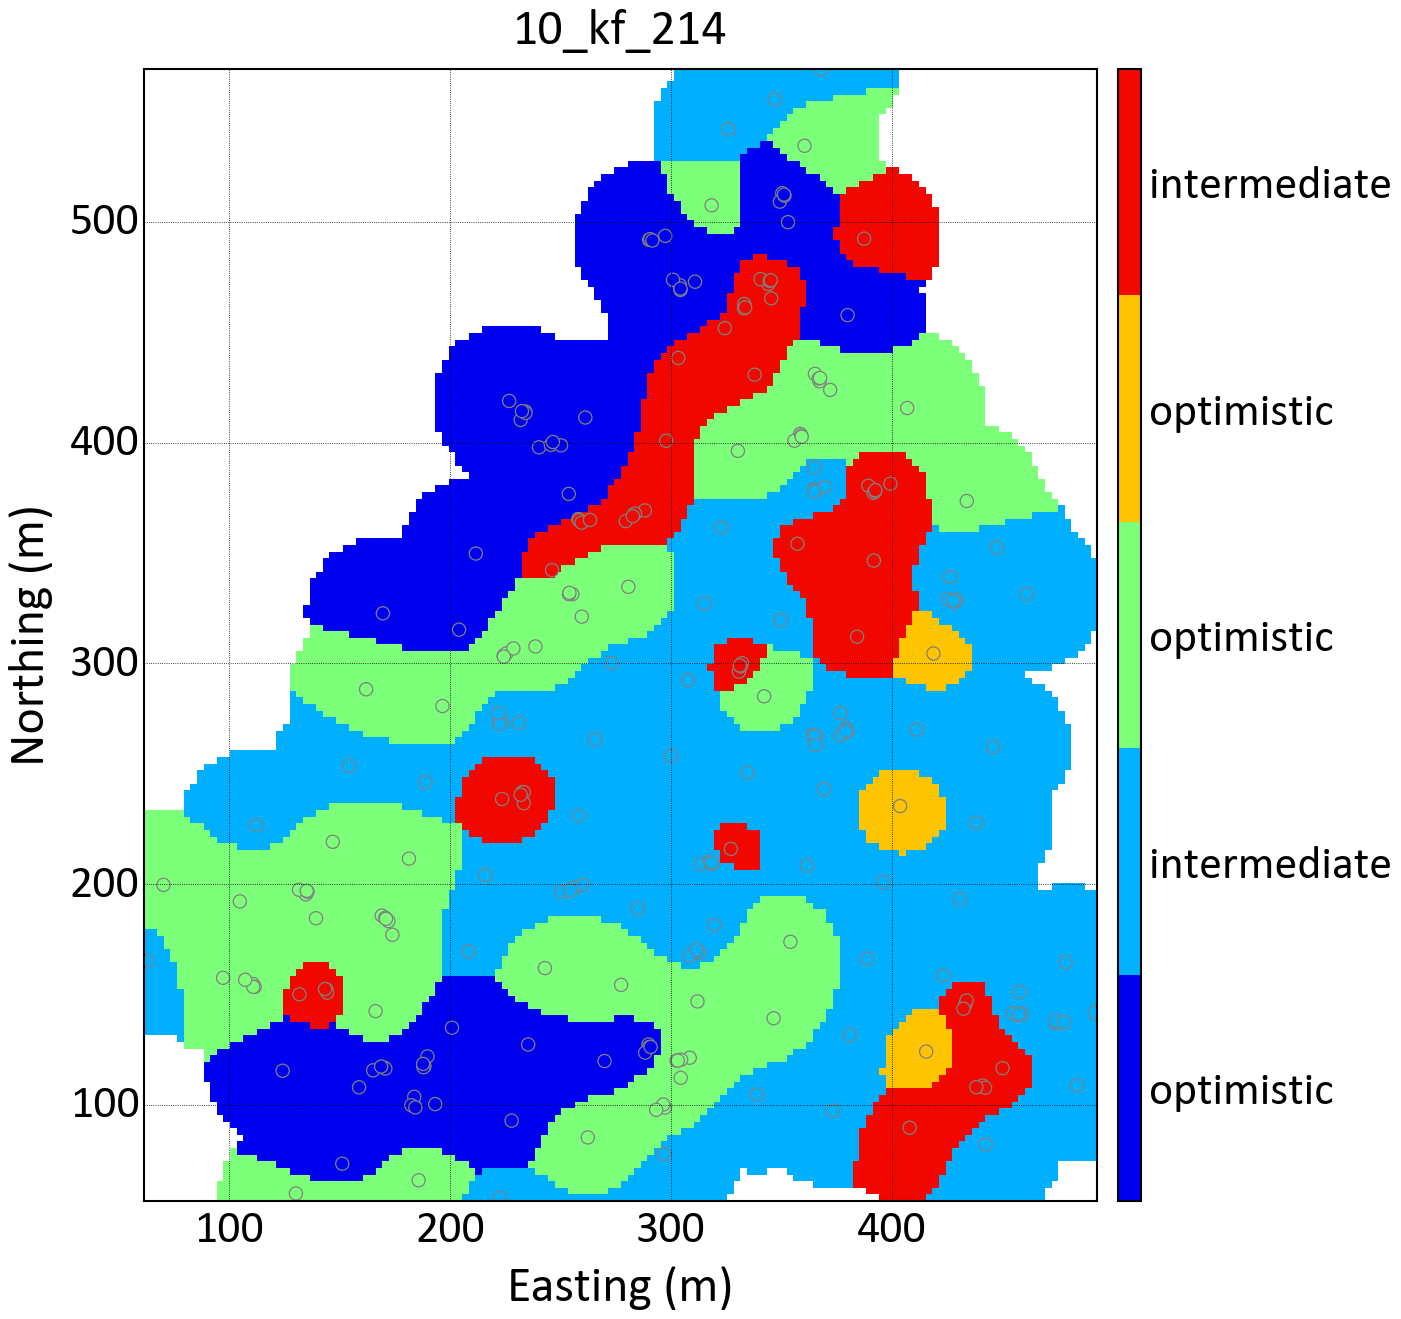
\includegraphics[width=.45\textwidth]{capitulo_3/imagens/out_model_10_kf_214.png}\label{<figure2>}}
\end{figure}

\subsection{Estudo de caso}

Pra ilustrar de forma prática a metodologia uma seção de um modelo conceitual foi desenvolvida e é mostrada na Figura \autoref{exa}. O modelo é composto por rocha encaixante, mostrada em vermelho, um dique, mostrado em verde, e estruturas lenticulares, mostradas em azul.

O modelo conceitual exaustivo  foi amostrado por 12 furos verticais igualmente espaçados. O espaçamento vertical das compostas é de 4 metros. O furos verticais são mostrados na Figura \autoref{sampl}. 

\begin{figure}[H] 
    \centering
    \caption{Modelo conceitual composto por rocha encaixante, mostrada em vermelho, um dique, mostrado em verde, e estruturas lenticulares, mostradas em azul.} \label{concep_exhaust}
     \subfloat[][Exaustivo.]{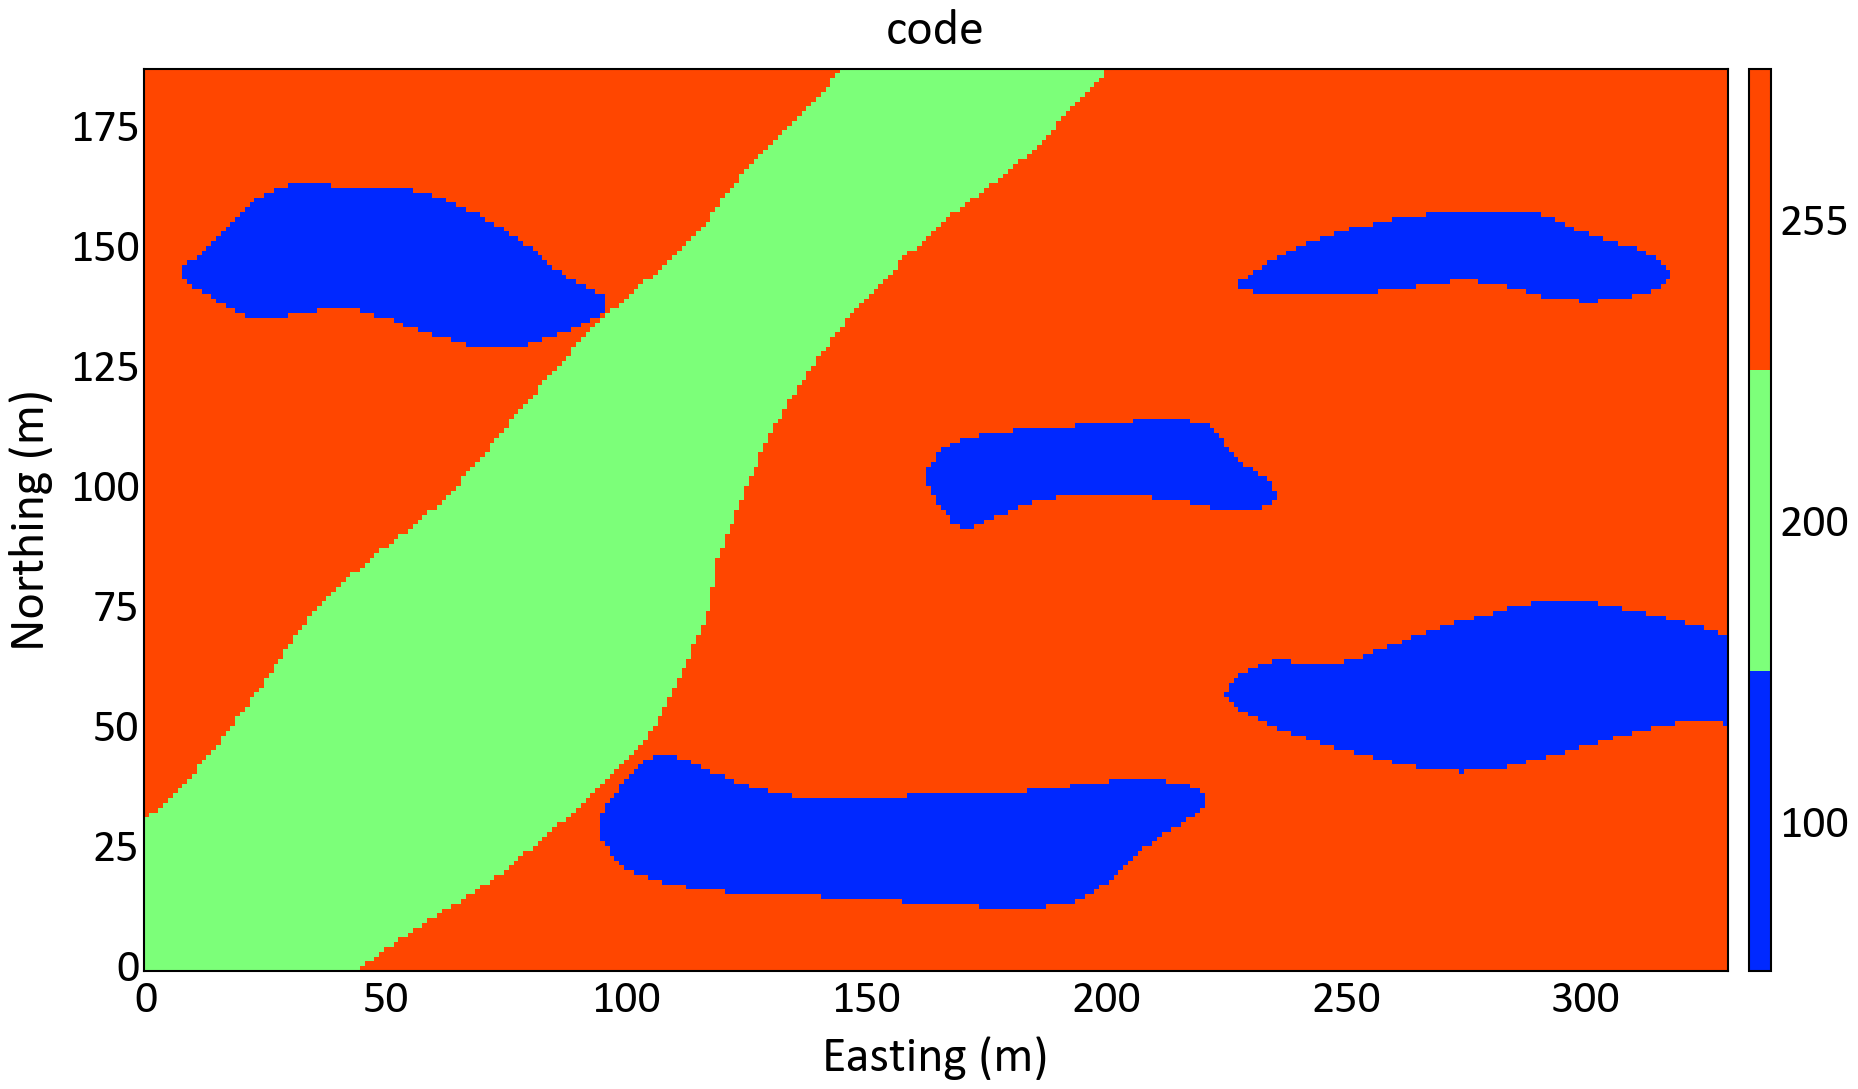
\includegraphics[width=.8\textwidth]{capitulo_3/imagens/exhaustive.png}\label{exa}}
     \\
     \subfloat[][Furos verticais.]{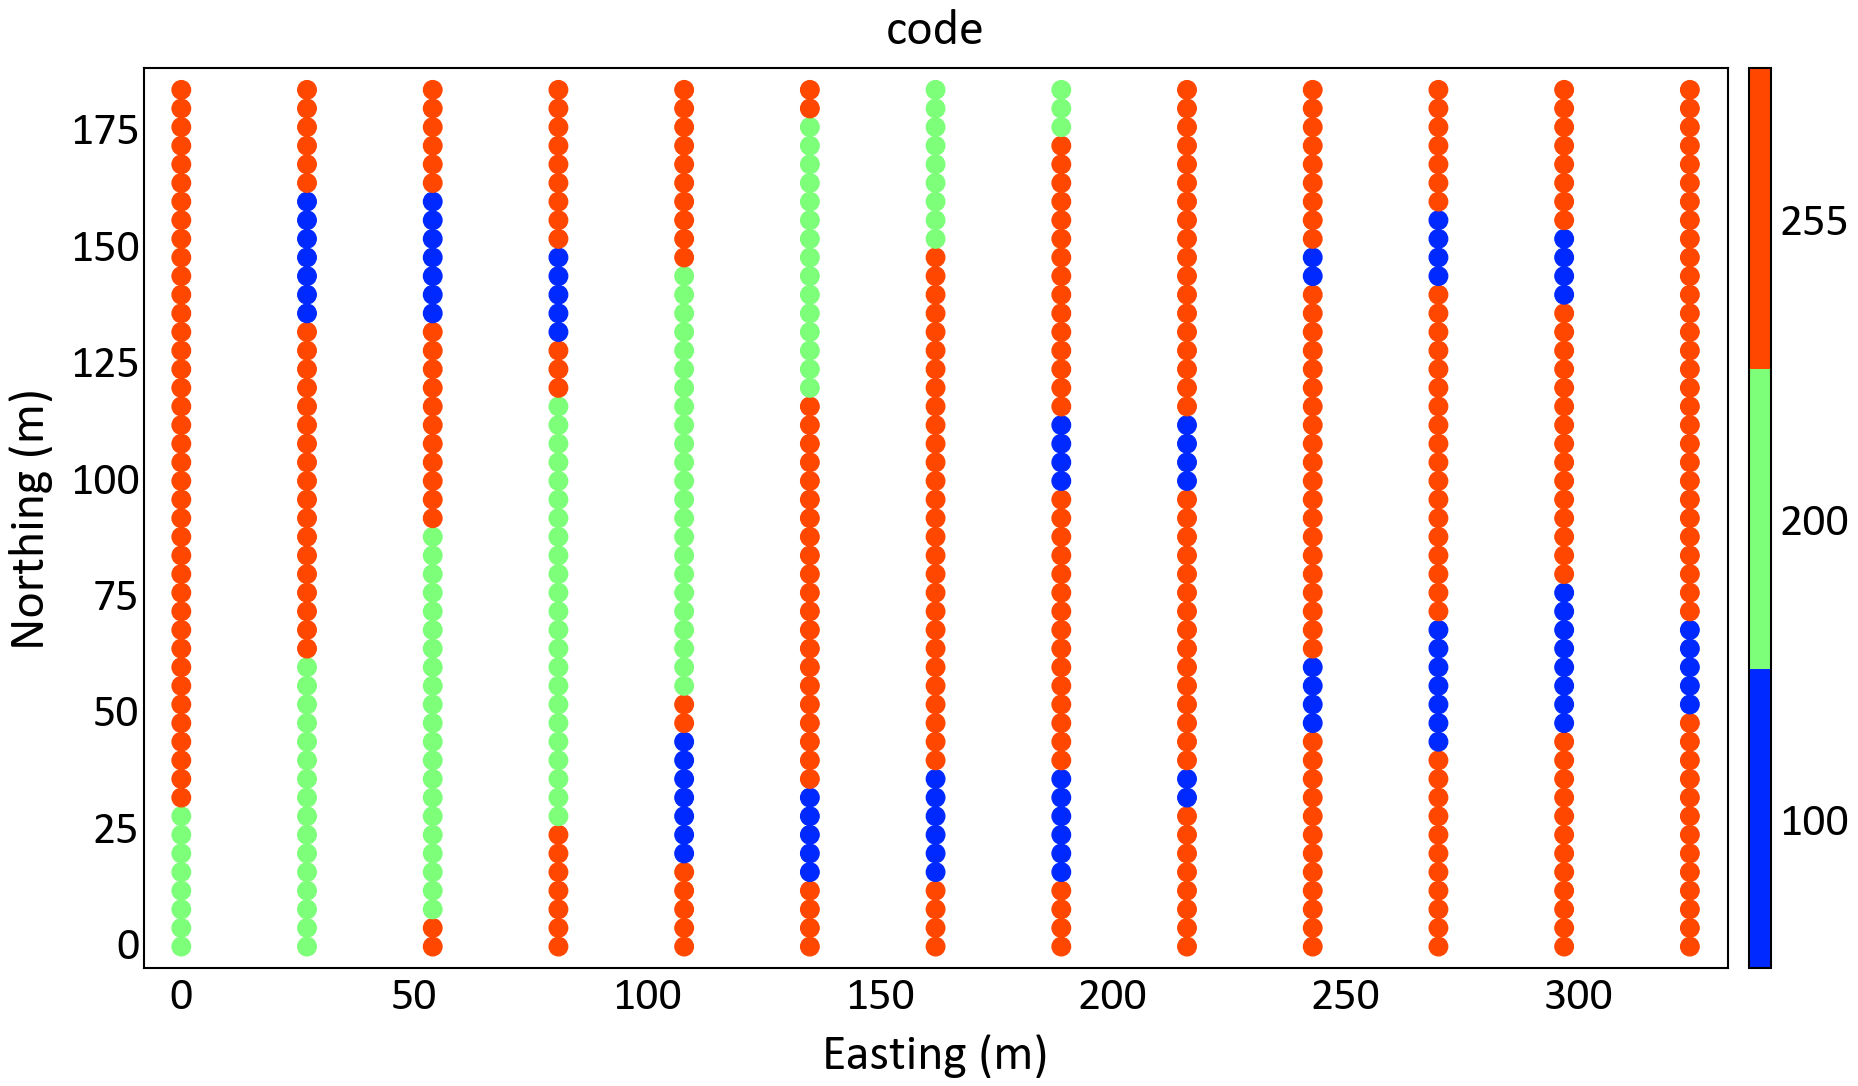
\includegraphics[width=.8\textwidth]{capitulo_3/imagens/sampled.png}\label{sampl}}
\end{figure}

O método foi aplicado no banco de dados da Figura \autoref{sampl}. O \textit{grid} de interpolação tem dimensões 1mx1m. O modelo dos \textit{kernels} é Gaussiano com suporte igual a 15 metros para todas as categorias. Não foi aplicada anisotropia e um efeito pepita de 0.01\% foi utilizado para evitar instabilidades nas matrizes.

Foi utilizada a parametrização linear com fmin otimista=fmin pessimista=0.8 e critério de aceitação de reprodução das amostras igual a 0.85.

A \autoref{synth_reals} mostra duas realizações aprovadas no critério de aceitação de reprodução dos dados amostrais escolhidas aleatoriamente.

Uma animação mostrando todas as realização (aprovadas no teste de reprodução) pode ser vista \href{https://github.com/robertorolo/kernel_support_parametrization_uncertainty_assess/blob/main/ezgif-6-114fcf125fa6.gif}{aqui}.

\begin{figure}[H] 
    \centering
    \caption{Realizações para o modelo geológico sintético gearadas a partir dos furos verticais.} \label{synth_reals}
     \subfloat[][Modelo 14.]{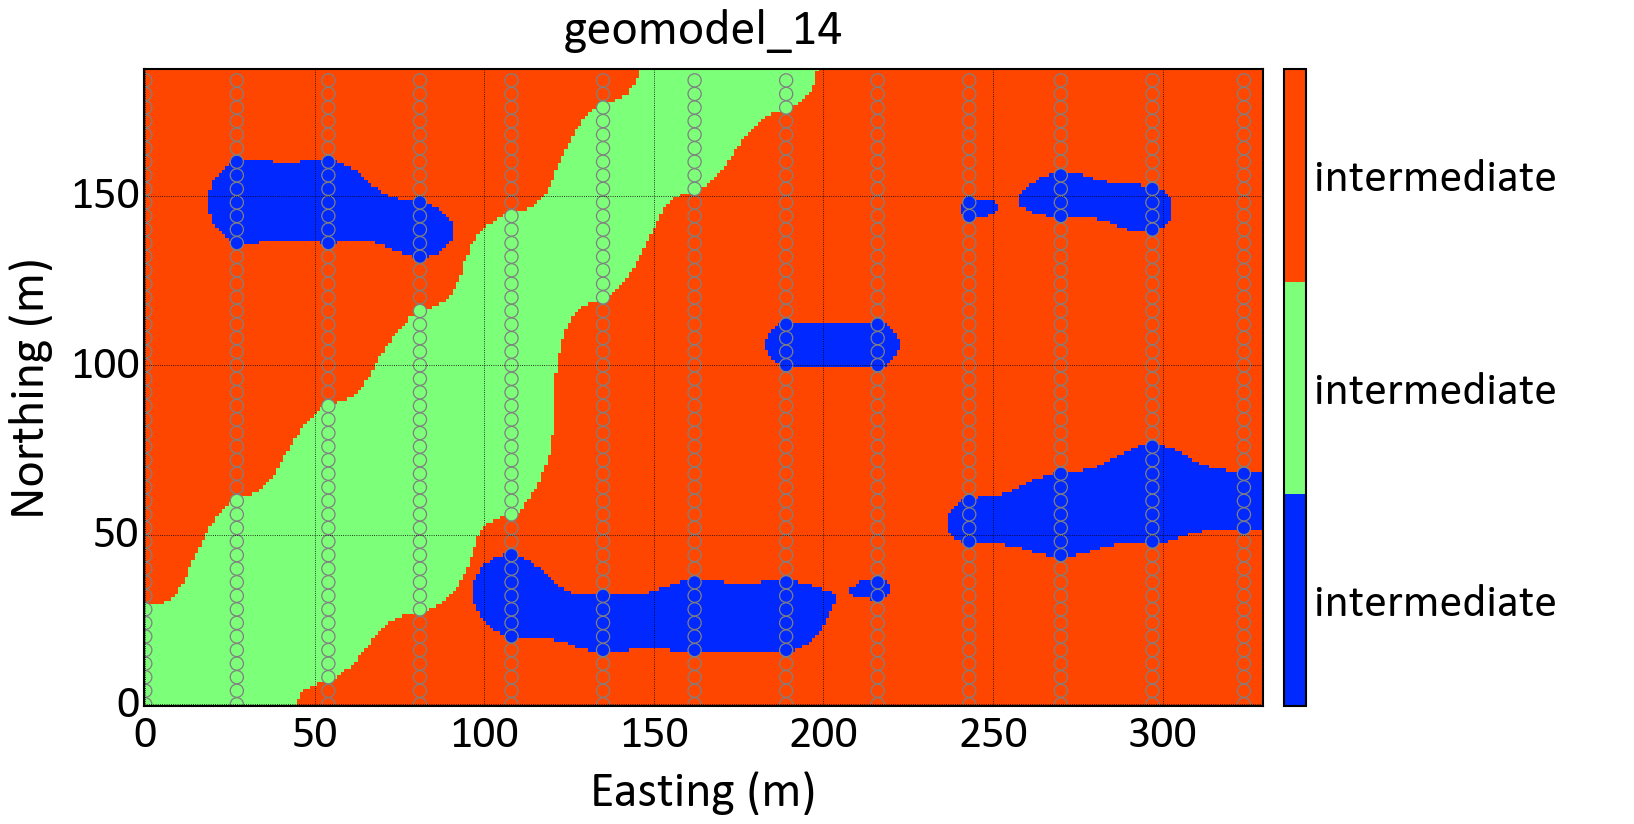
\includegraphics[width=.8\textwidth]{capitulo_3/imagens/drill_holes_out_model_geomodel_13.png}\label{mod20}}
     \\
     \subfloat[][Modelo 21.]{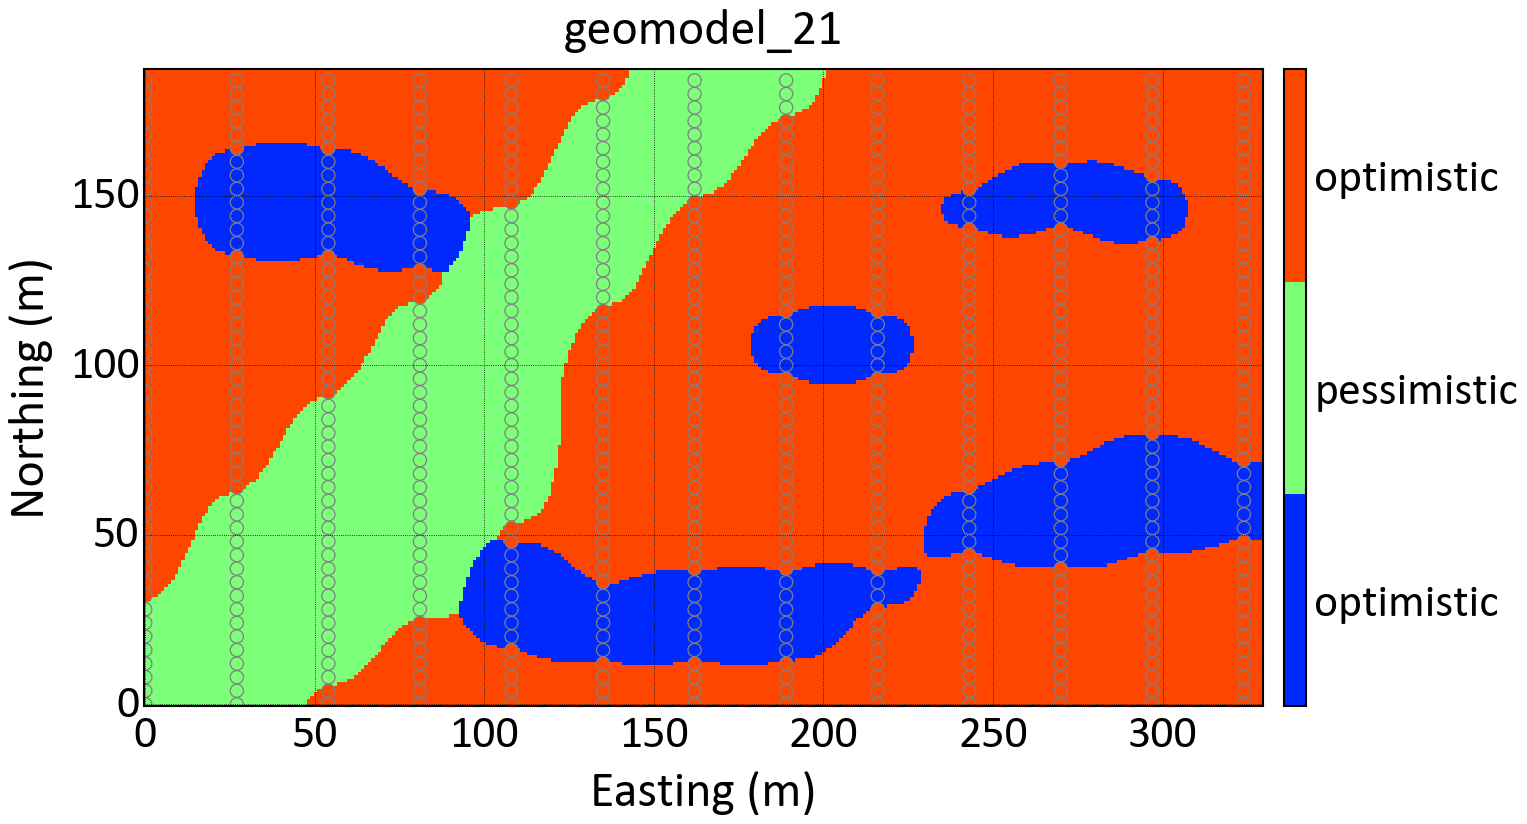
\includegraphics[width=.8\textwidth]{capitulo_3/imagens/drill_holes_out_model_geomodel_21.png}\label{mod21}}
\end{figure}

\subsection{Discussão}

O método proposto por \citeonline{mclennanstationarity} é baseado em interpoladores pelo inverso da distância. Por esse motivo, não é possível considerar anisotropia nos modelos. O autor põe o método em prática apenas em modelos sintéticos de geometria simples, quando aplicado à modelos com geologias complexas a multiplicação dos pesos diretamente pelo fator calculado para cada amostra a partir da parametrização produziu, muitas vezes, volumes (ou áreas) muito grandes ou muito pequenas que não honram os dados amostrais. Aplicar o fator no suporte do \textit{kernel} torna o método menos sensível aos fatores e dá ao usuário um controle maior sobre os modelos gerados, já que é possível diminuir artificialmente o suporte do \textit{kernel} para diminuir sua influência em detrimento da influência da parametrização.

O método proposto, por ser baseado em interpolação global, gera modelos sem ruídos e apresentando o realismo geológico esperado. O método simula diferentes interpretações para o modelo geológico nas quais o volume de cada litologia é maior ou menor em relação aos demais cenários.

O usuário pode controlar o quanto os modelos honram os dados amostrais, entretanto, uma maior restrição nesse sentido gera menos cenários diferentes.

\section{Avaliação de incerteza usando funções distância assinaladas e campos de probabilidades}

\citeonline{froidevaux1993probability} propôs uma abordagem para simulação condicional de variáveis contínuas. Este método dissocia a tarefa de estimar as funções de distribuição de probabilidade local (PDFs) da produção de realizações equiprováveis. A simulação do campo de probabilidade começa com a premissa de que as distribuições condicionais locais são conhecidas. As simulações condicionais são então obtidas extraindo realizações desses PDFs.

A metodologia proposta usa essa premissa para simular contatos. A primeira etapa é definir uma largura de banda de incerteza em torno dos contatos. Como não há incerteza dentro dos domínios, os blocos fora da zona de incerteza são congelados como a categoria responsável pela distância assinalada estimada mais negativa. Simultaneamente, os blocos dentro da zona de incerteza serão classificados como diferentes categorias em diferentes realizações.

A largura de banda pode ser definida por um geomodelador com base no tipo de depósito e configuração amostral: em depósitos onde a geologia apresenta variabilidade mais significativa, como depósitos com múltiplas rochas intrusivas, ela deve ser mais ampla; em depósitos menos erráticos, como os estratificados, deve ser mais estreito. Em configurações de amostragem com espaçamento próximo, zonas menores de incerteza são necessárias, enquanto em configurações de amostragem esparsas, zonas mais amplas são necessárias.

A distância assinalada estimada é a distância de um bloco ao domínio oposto mais próximo. A zona de incerteza é definida pela retenção de todos os blocos onde o valor absoluto da distância estimada de pelo menos uma categoria é menor ou igual ao valor definido pelo geomodelador para a largura de banda de incerteza.

A estimativa da pdf local é feita transformando as distâncias estimadas em probabilidades como mostrado na \autoref{heuristic}.

A partir da modelagem multi categórico no banco de dados \textit{Swiss Jura} mostrada na \autoref{multicat_jura} foi determinada uma zona de incerteza de 12 metros ao redor dos contatos. Isto é, Para cada uma das distâncias assinaladas interpoladas que representam cada uma das categorias do banco de dados, qualquer bloco em que a distância interpolada pertença ao intervalo [-12,12] é classificado como zona de incerteza.

A \autoref{unc_zone} mostra, do lado esquerdo, blocos definidos como pertencentes à banda de incerteza de 12 metros para o \textit{Swiss Jura}. As cores indicam quantas categorias têm sua distância assinalada interpolada absoluta menor ou igual ao valor da largura de banda (12 metros).

\begin{figure}[H]
	\caption{\label{unc_zone} Da esquerda para a direita: (1) zona de incerteza de 12 metros; (2) distâncias estimadas para um bloco específico; (3) probabilidades transformadas.}
	\centering
		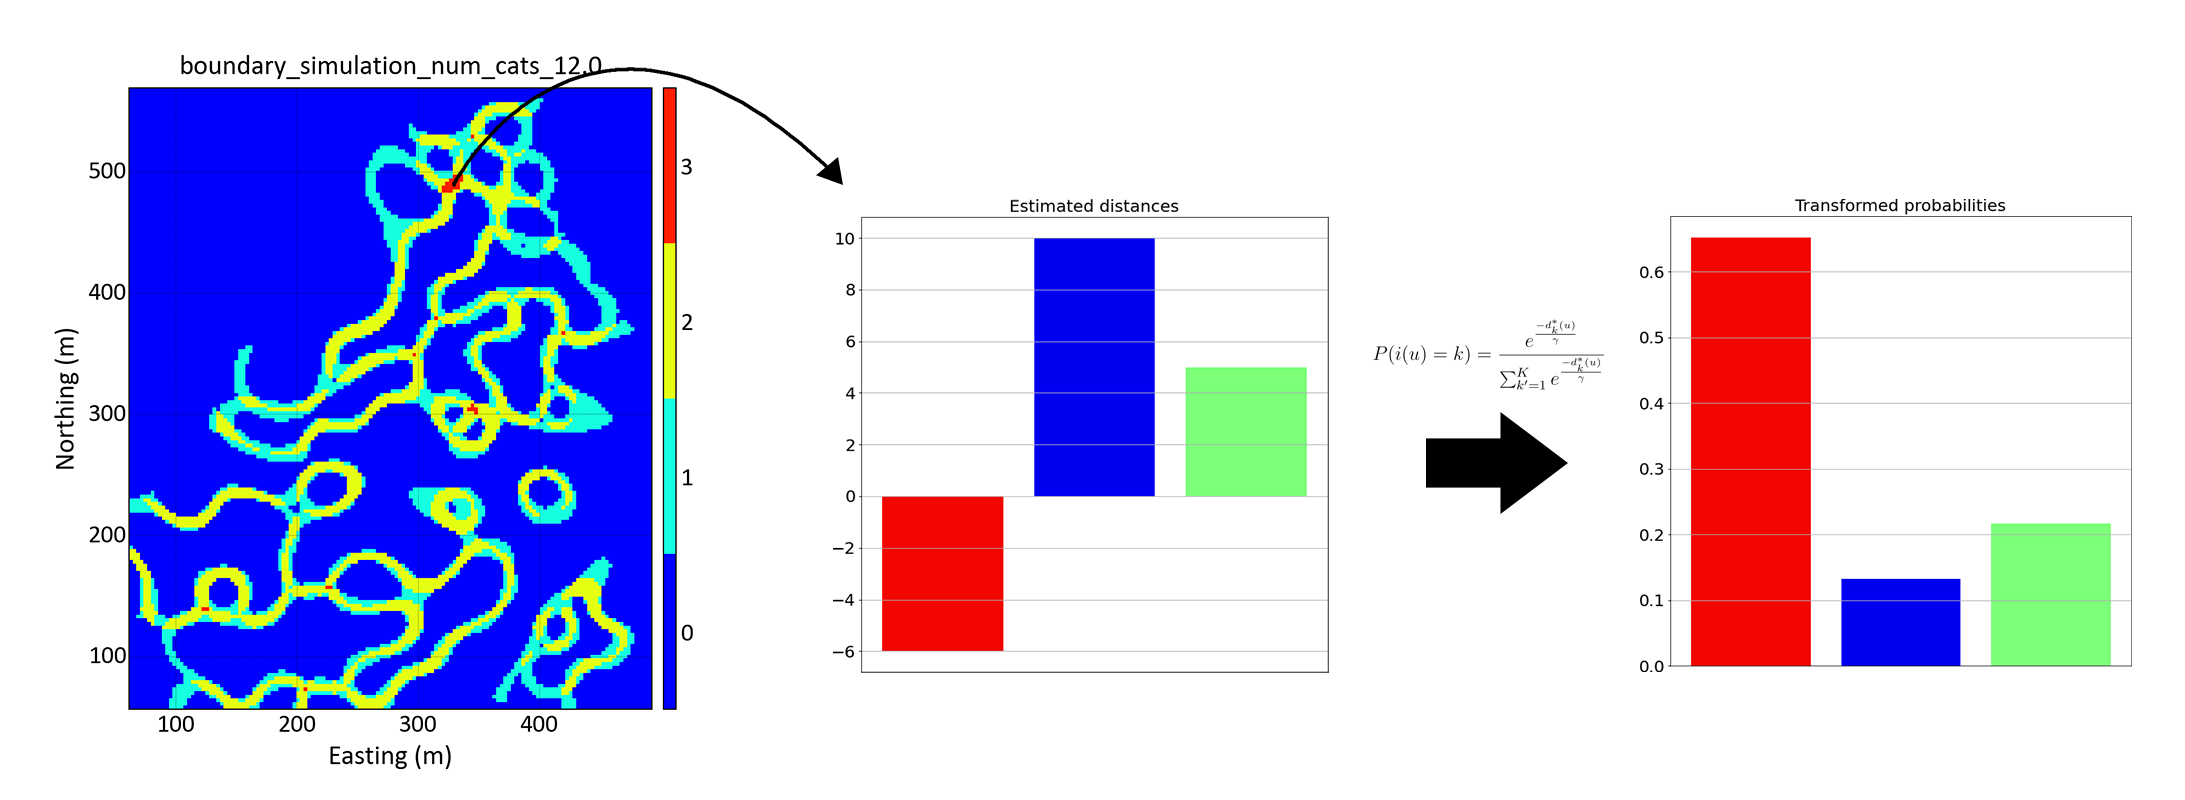
\includegraphics[width=\textwidth]{capitulo_3/imagens/trans_dist_prob.png}
\end{figure}

Observe que, embora haja cinco categorias diferentes no banco de dados, apenas três farão parte da distribuição de probabilidade local em um bloco vermelho; apenas dois em um bloco amarelo e apenas um em um bloco azul claro. A imagem central mostra as distâncias estimadas para um bloco específico. Finalmente, no lado direito estão as probabilidades transformadas pelo \autoref{eq_softmax} para aquele bloco específico usando o valor de distância absoluta máxima como o parâmetro $\omega$.

A produção de realizações equiprováveis para o modelo geológico é feita simulando primeiro um campo gaussiano incondicional dentro da zona de incerteza por simulação gaussiana sequencial como mostrado no \autoref{algo:usgs}. Os valores gaussianos devem ser transformados no campo de probabilidade normalizando-os para variar entre 0 e 1 em uma distribuição uniforme. Isso é feito calculando os valores de distribuição normal cumulativos.

Finalmente, para gerar várias realizações, uma categoria deve ser amostrada da pdf local usando o campo de probabilidade simulado para cada bloco dentro da zona de incerteza em cada realização, como mostrado na \autoref{samplig_from_dist}.

\begin{figure}[H]
	\caption{\label{samplig_from_dist} Um valor de probabilidade simulado de 0,51 é usado para amostrar a categoria vermelha de uma distribuição condicional em um bloco específico.}
	\centering
		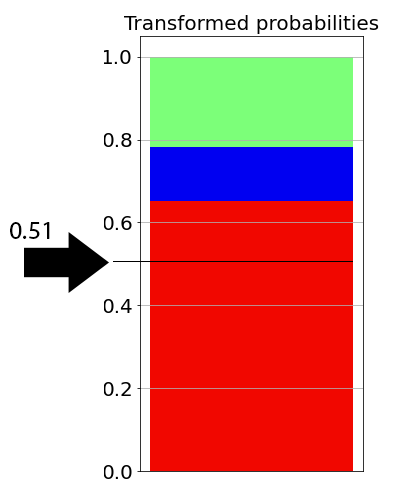
\includegraphics[width=0.3\textwidth]{capitulo_3/imagens/sampling_from_dist.png}
\end{figure}

A \autoref{reals_pfield_jura} mostra, do lado esquerdo, duas realizações diferentes de uma simulação Gaussiana incondicional dentro da zona de incerteza. Ao lado direito mostra duas realizações do modelo geológico criado pela amostragem de uma categoria das distribuições condicionais para o banco de dados \textit{Swiss Jura}. A transição entre as diferentes categorias é suave, pois as simulações Gaussianas têm continuidade espacial. Uma animação mostrando todas as 10 realizações realizadas pode ser vista \href{https://github.com/robertorolo/assessing_geological_model_uncertainty_with_probability_fields/blob/main/jura_gif.gif}{aqui}.

\begin{figure}[H]
	\caption{\label{reals_pfield_jura} Realizações Gaussianas e modelos geológicos correspondentes.}
	 \centering
     \subfloat[][Realização Gaussiana 1]{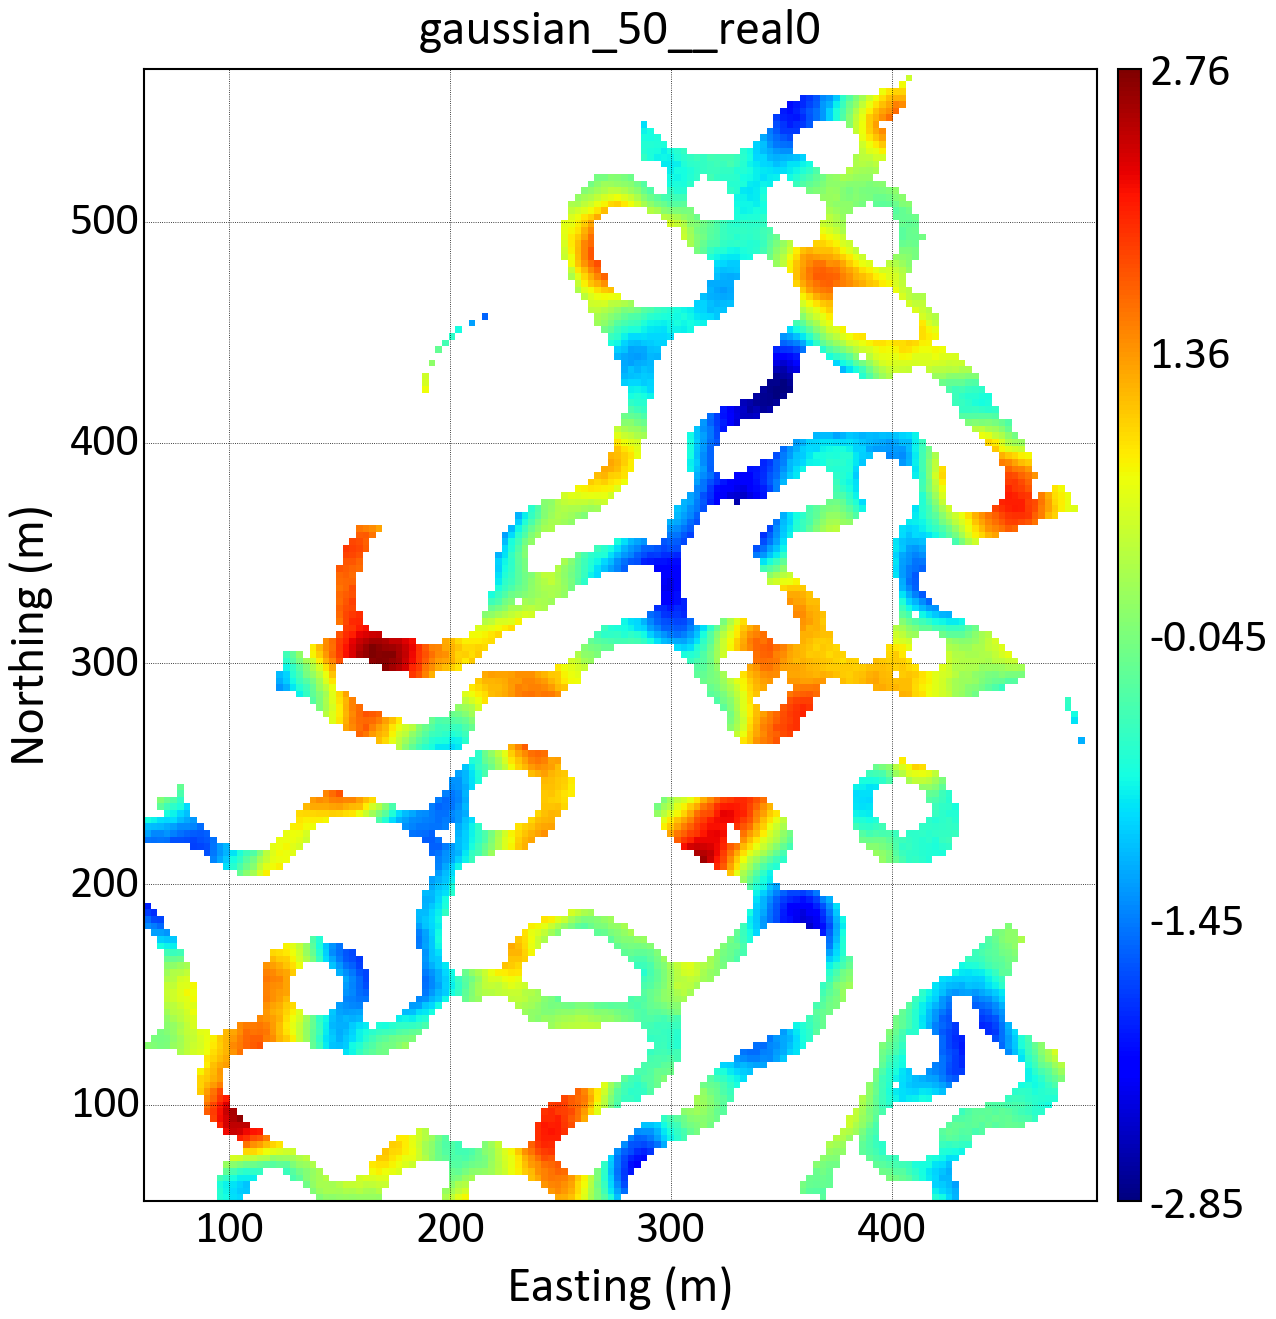
\includegraphics[height=150pt]{capitulo_3/imagens/gausssim_0_12.png}\label{fig:g1}}
     \hspace{1em}
     \subfloat[][Realização do modelo geológico 1]{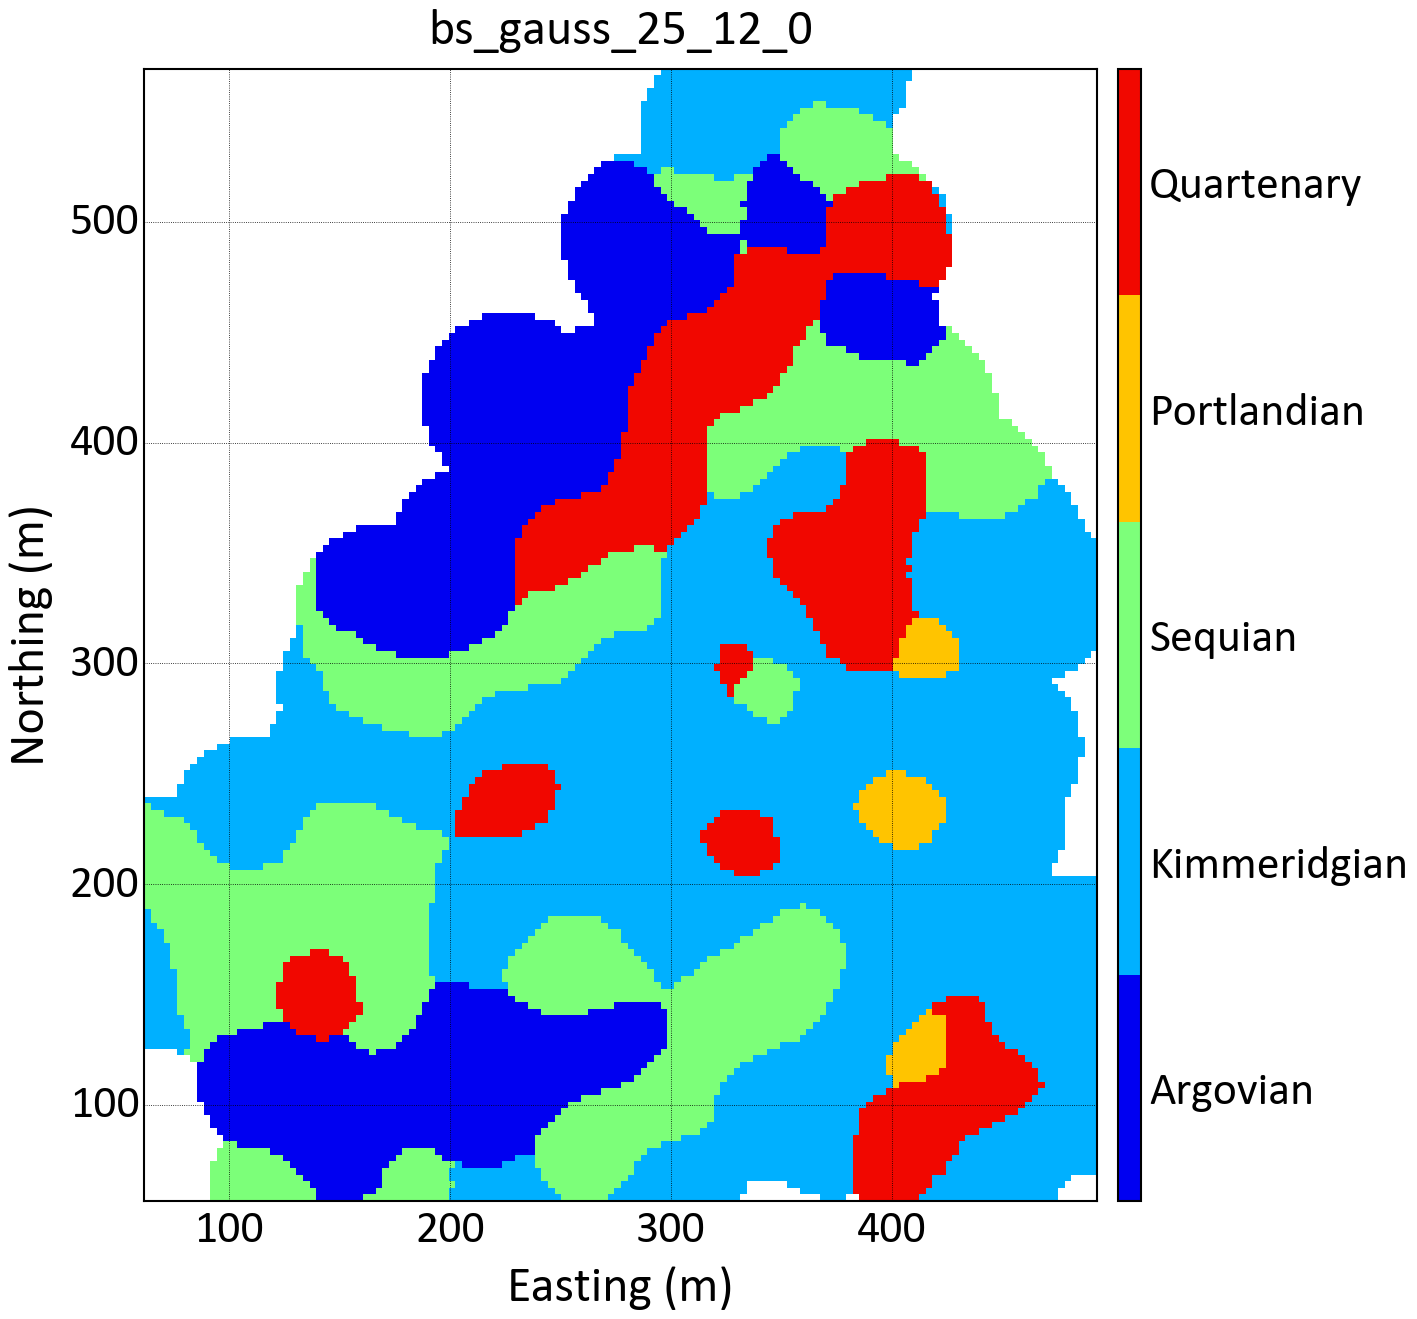
\includegraphics[height=150pt]{capitulo_3/imagens/gauss_real_0_25_12.png}\label{fig:g2}}\\
     \subfloat[][Realização Gaussiana 2]{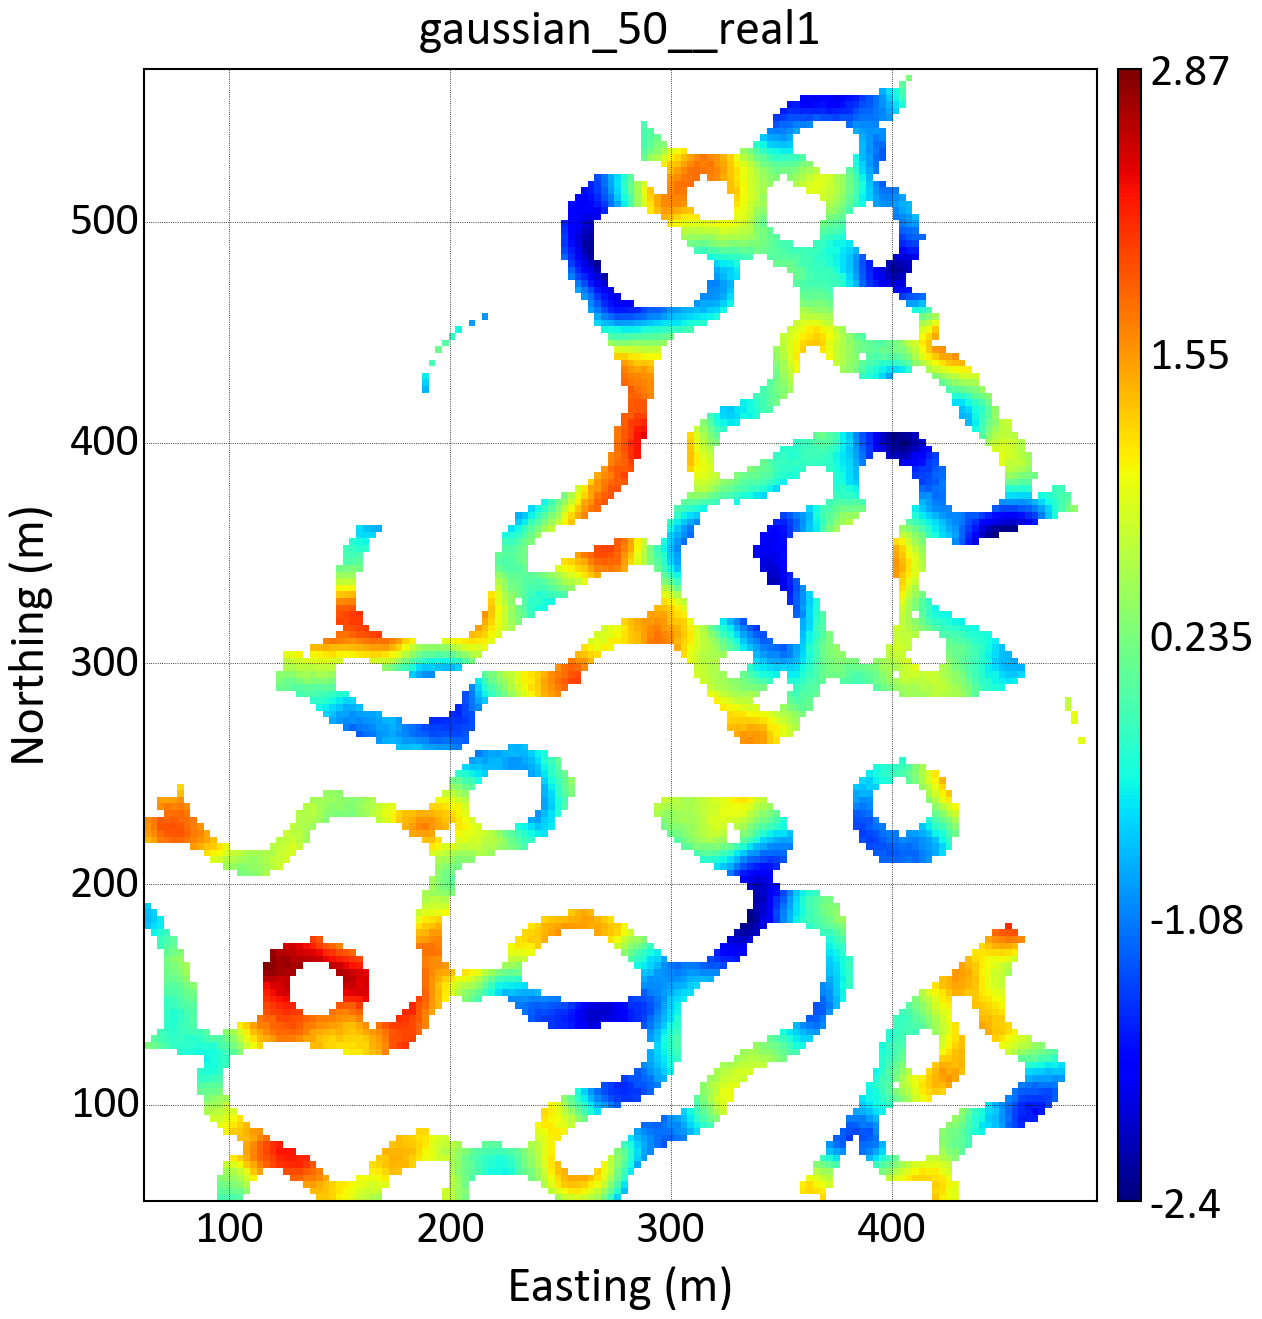
\includegraphics[height=150pt]{capitulo_3/imagens/gausssim_1_12.png}\label{fig:g3}}
     \hspace{1em}
     \subfloat[][Realização do modelo geológico 2]{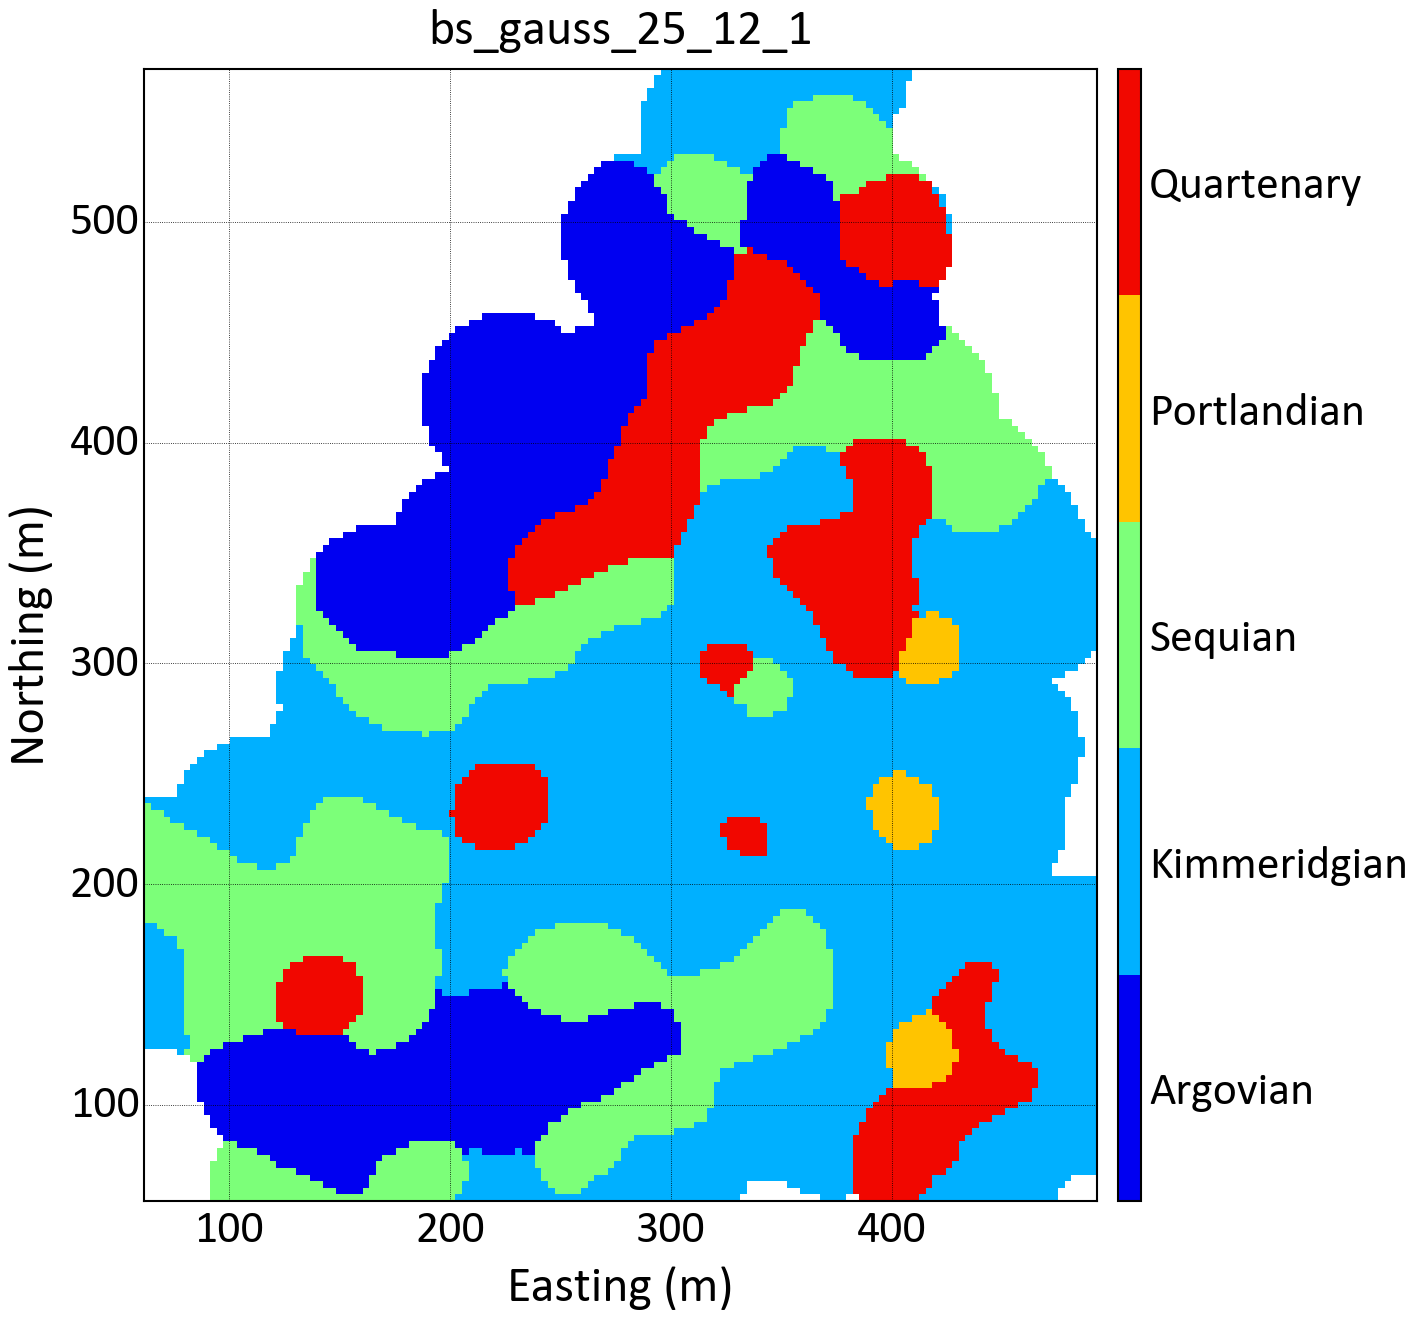
\includegraphics[height=150pt]{capitulo_3/imagens/gauss_real_1_25_12.png}\label{fig:g4}}
\end{figure}

\subsection{Estudo de caso}

Este estudo de caso foi conduzido em um banco de dados real fornecido por uma grande operação de mineração de ouro. O conjunto de dados apresenta 9140 amostras em suporte pontual representando cinco litologias diferentes localizadas em uma área de aproximadamente 10 km² com 1300 metros de profundidade. Uma vista isométrica das amostras pode ser vista na \autoref{ouro_amost}.

\begin{figure}[H]
	\caption{\label{ouro_amostras} Vista isométrica das amostras do depósito de ouro.}
	\centering
		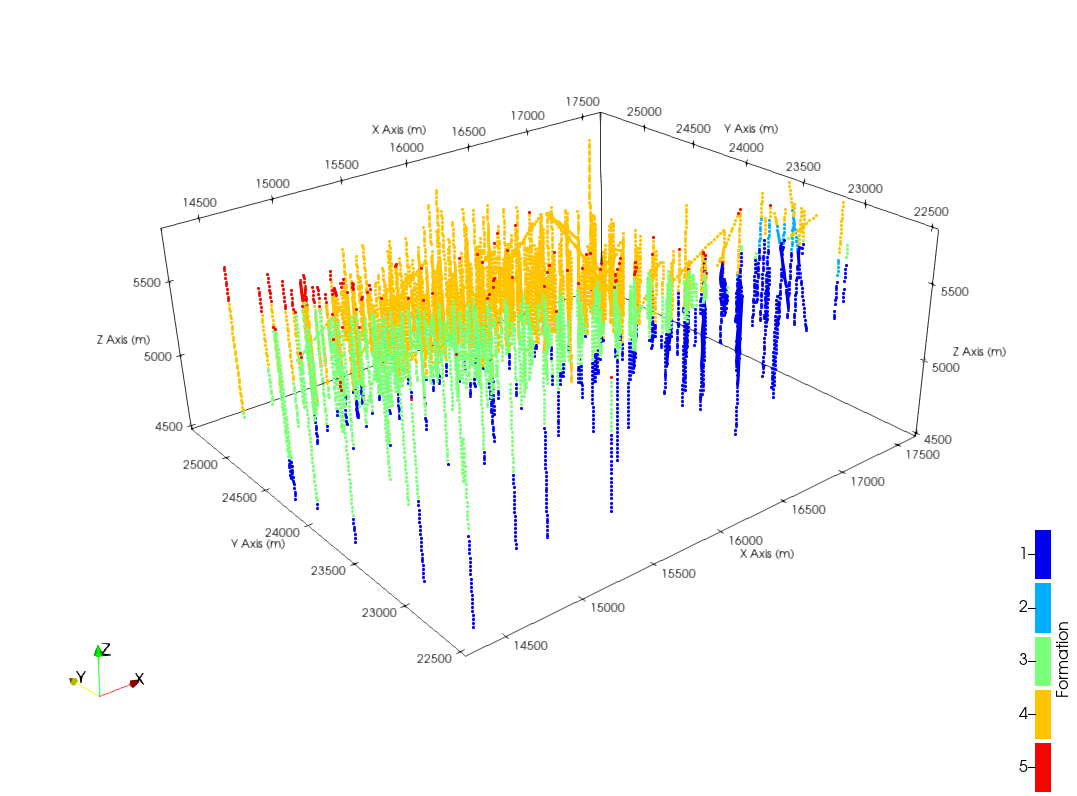
\includegraphics[width=0.8\textwidth]{capitulo_3/imagens/points_perpect.png}
\end{figure}

\citeonline{rolo_dissertacao} e \citeonline{rolo2017signed} realizaram um estudo de caso no mesmo banco de dados, no entanto, esses autores usaram distâncias assinaladas para criar um modelo geológico multi-categórico determinístico. O presente trabalho é uma extensão natural do trabalho acima mencionado, uma vez que é simples e direto avaliar a incerteza do modelo geológico usando campos de probabilidade a partir das distâncias estimadas usadas para modelagem geológica determinística.

As distâncias assinaladas devem ser interpoladas para todas as cinco categorias. O variograma das distâncias mostra um comportamento não estacionário e, portanto, não atinge um patamar. Uma alternativa é modelar os variogramas dos indicadores, que são estacionários, e usar um equivalente gaussiano para interpolação de distância. É recomendado o uso de um modelo Gaussiano, pois seu comportamento parabólico próximo à origem leva a limites geológicos suaves e realistas. 

Os variogramas dos indicadores para as cinco categorias do depósito de ouro foram calculados e modelados com estruturas esféricas, conforme mostrado na \autoref{ouro_vargs}.  

\begin{figure}[H]
    \caption{Variogramas dos indicadores para todas as cinco categorias do depósito mineral modelados com estruturas esféricas.} \label{ouro_vargs}
     \centering
     \subfloat[][Variograma omni horizontal em azul e vertical em vermelho para a categoria 1.]{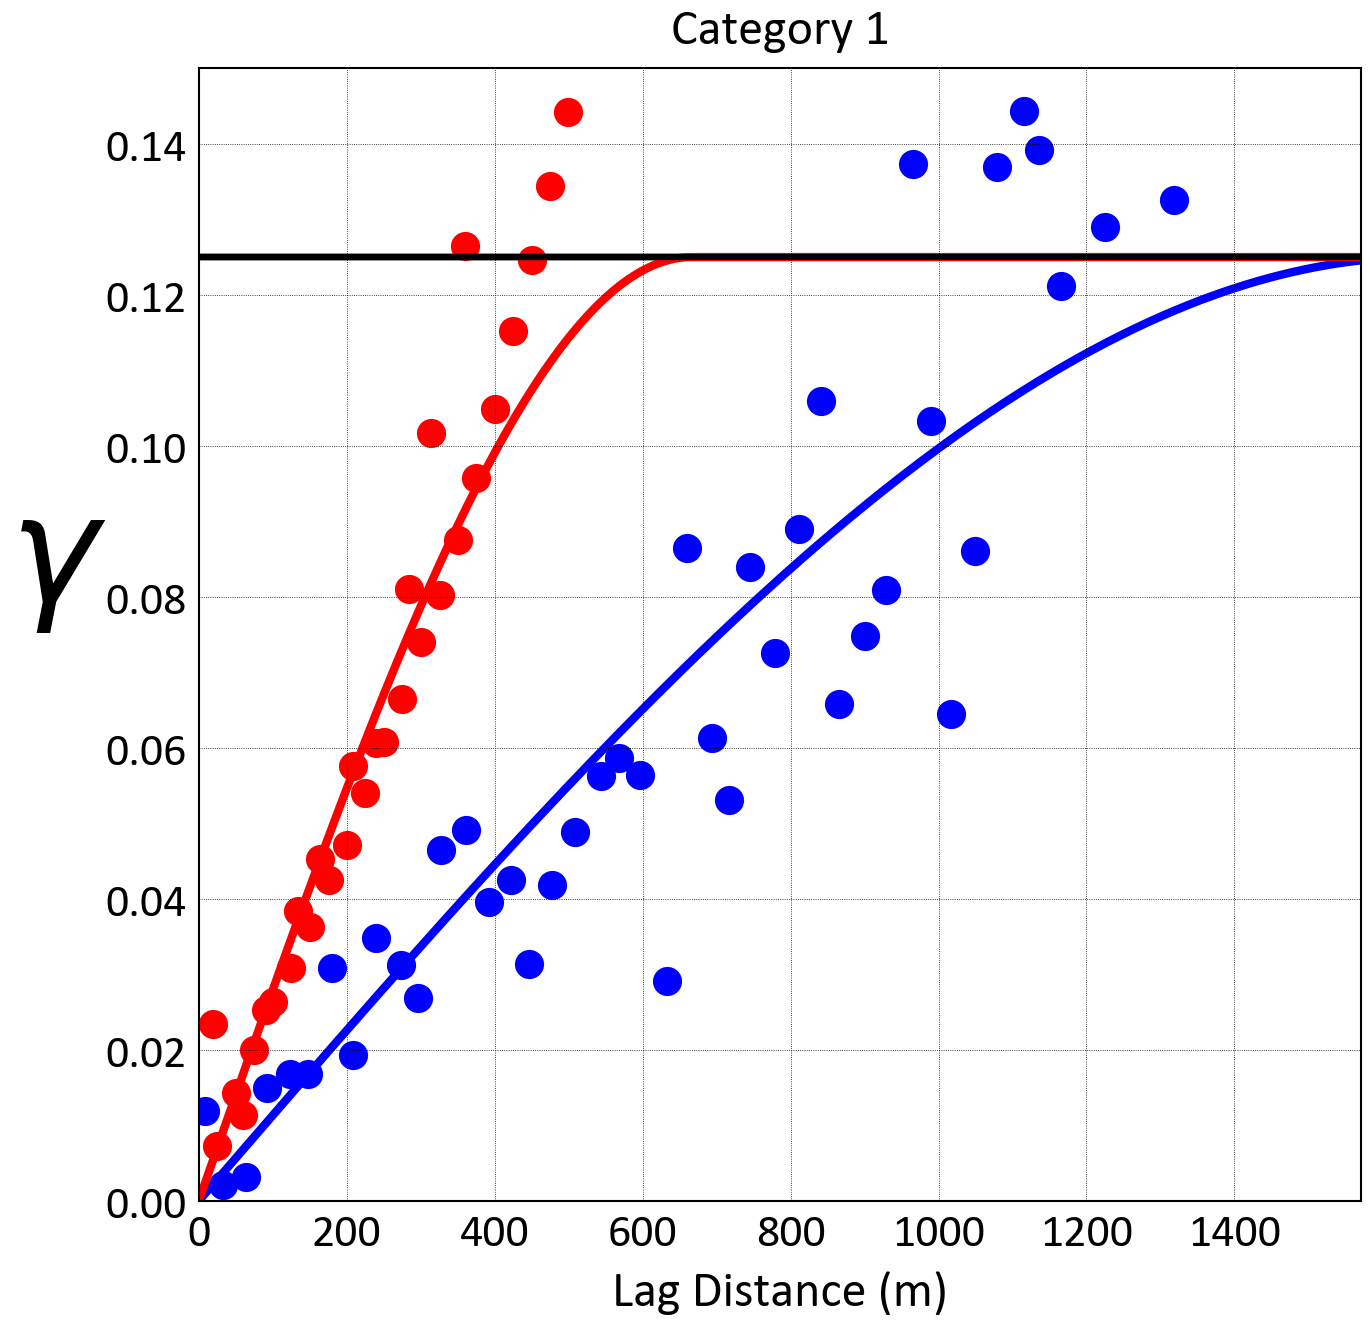
\includegraphics[height=150pt]{capitulo_3/imagens/var_1.png}\label{fig:v1}}
     \hspace{1em}
     \subfloat[][Variograma omnidirecional para a categoria 2.]{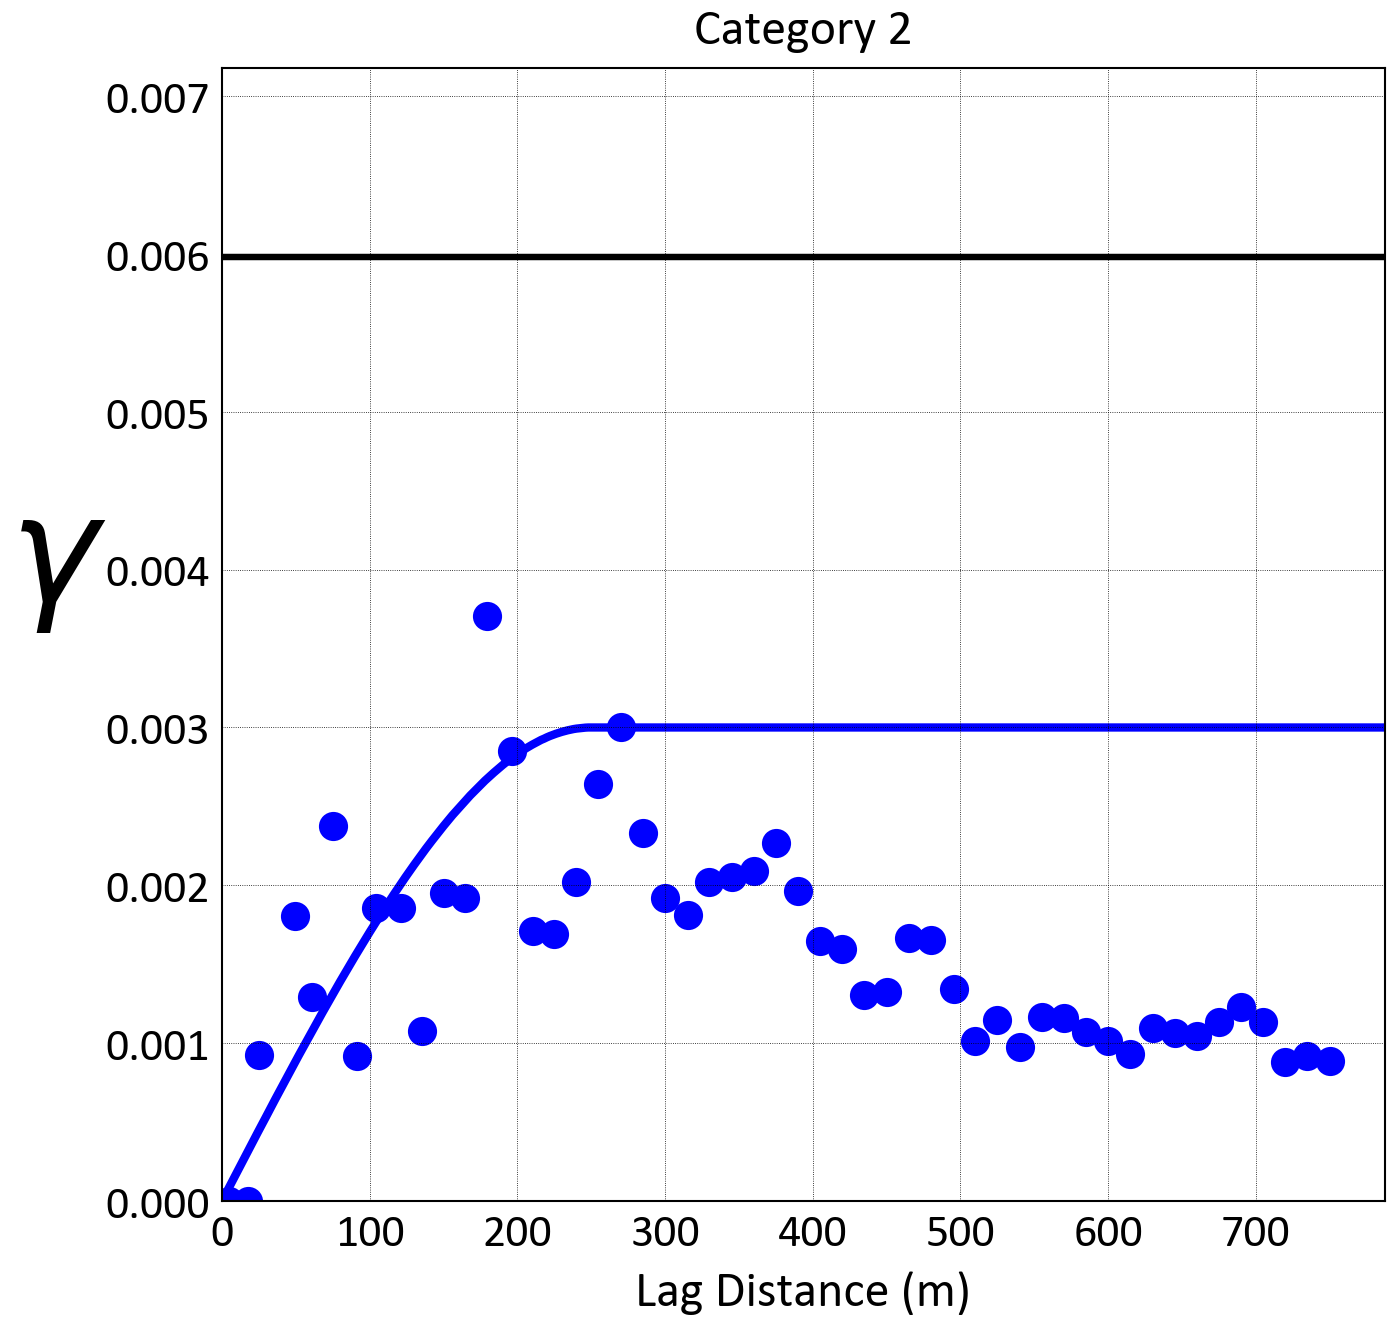
\includegraphics[height=150pt]{capitulo_3/imagens/var_2.png}\label{fig:v2}}\\
    \subfloat[][Variograma omnidirecional para a categoria 3.]{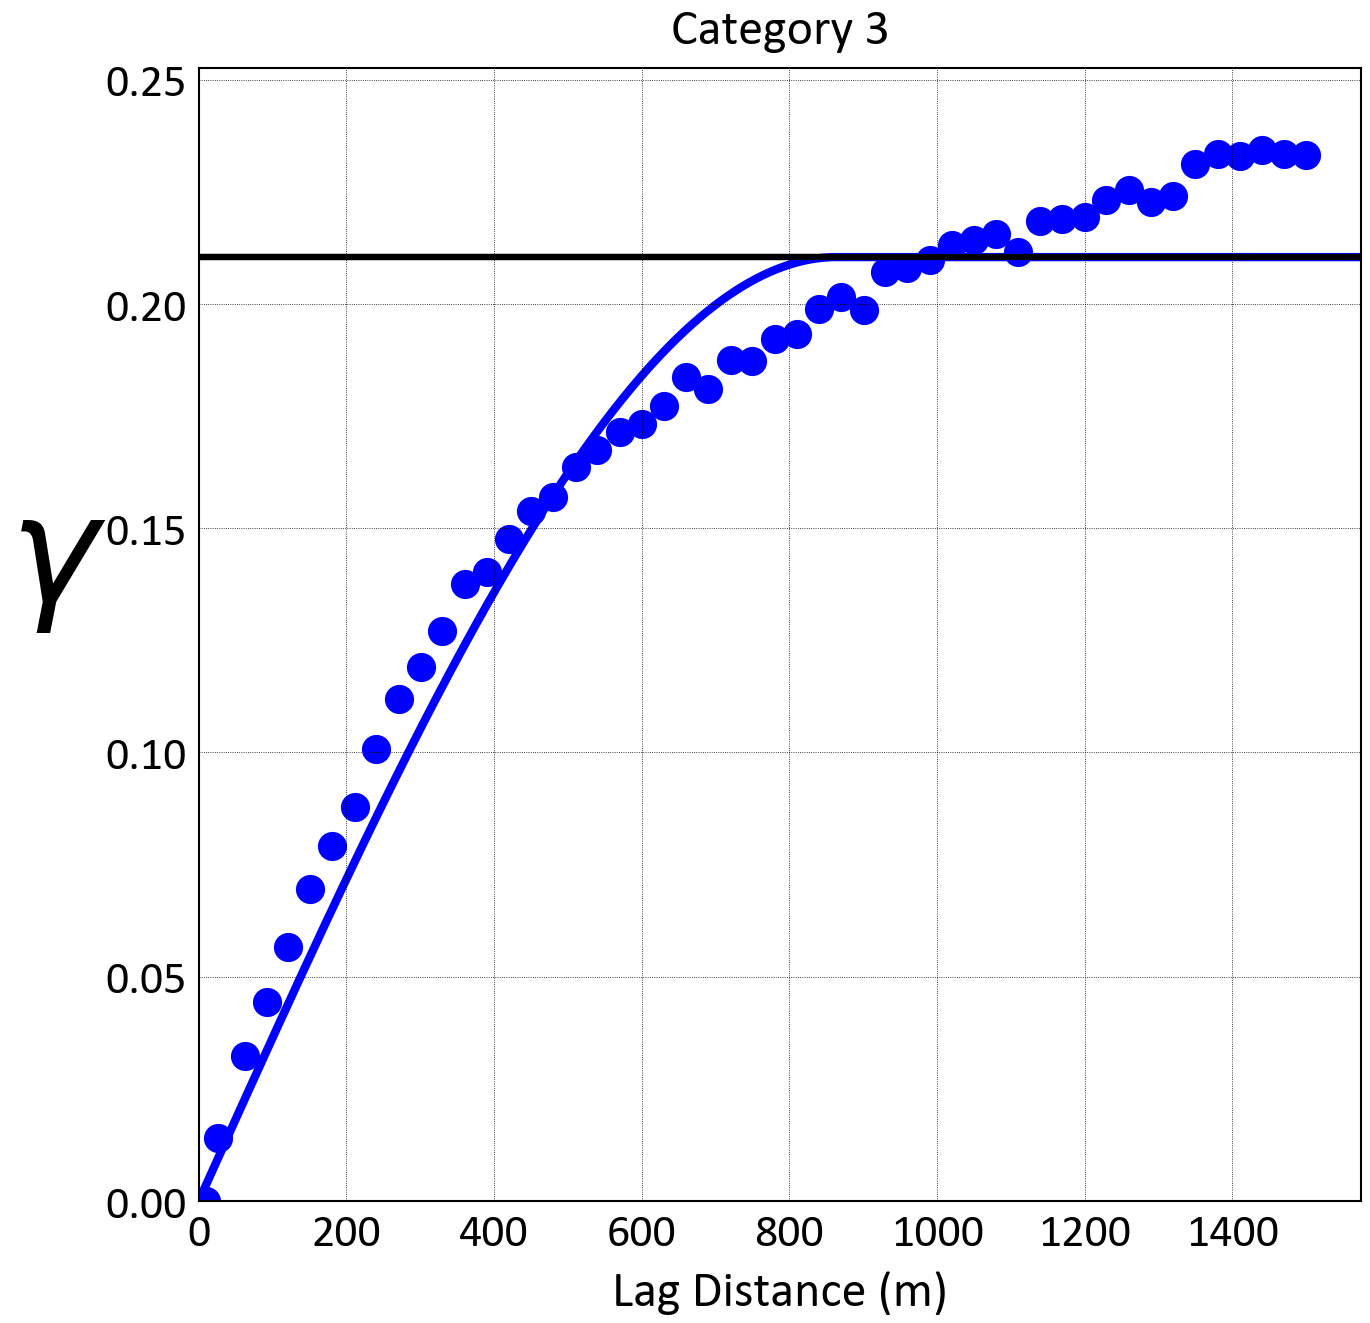
\includegraphics[height=150pt]{capitulo_3/imagens/var_3.png}\label{fig:v3}}
    \hspace{1em}
    \subfloat[][Variograma omnidirecional para a categoria 4.]{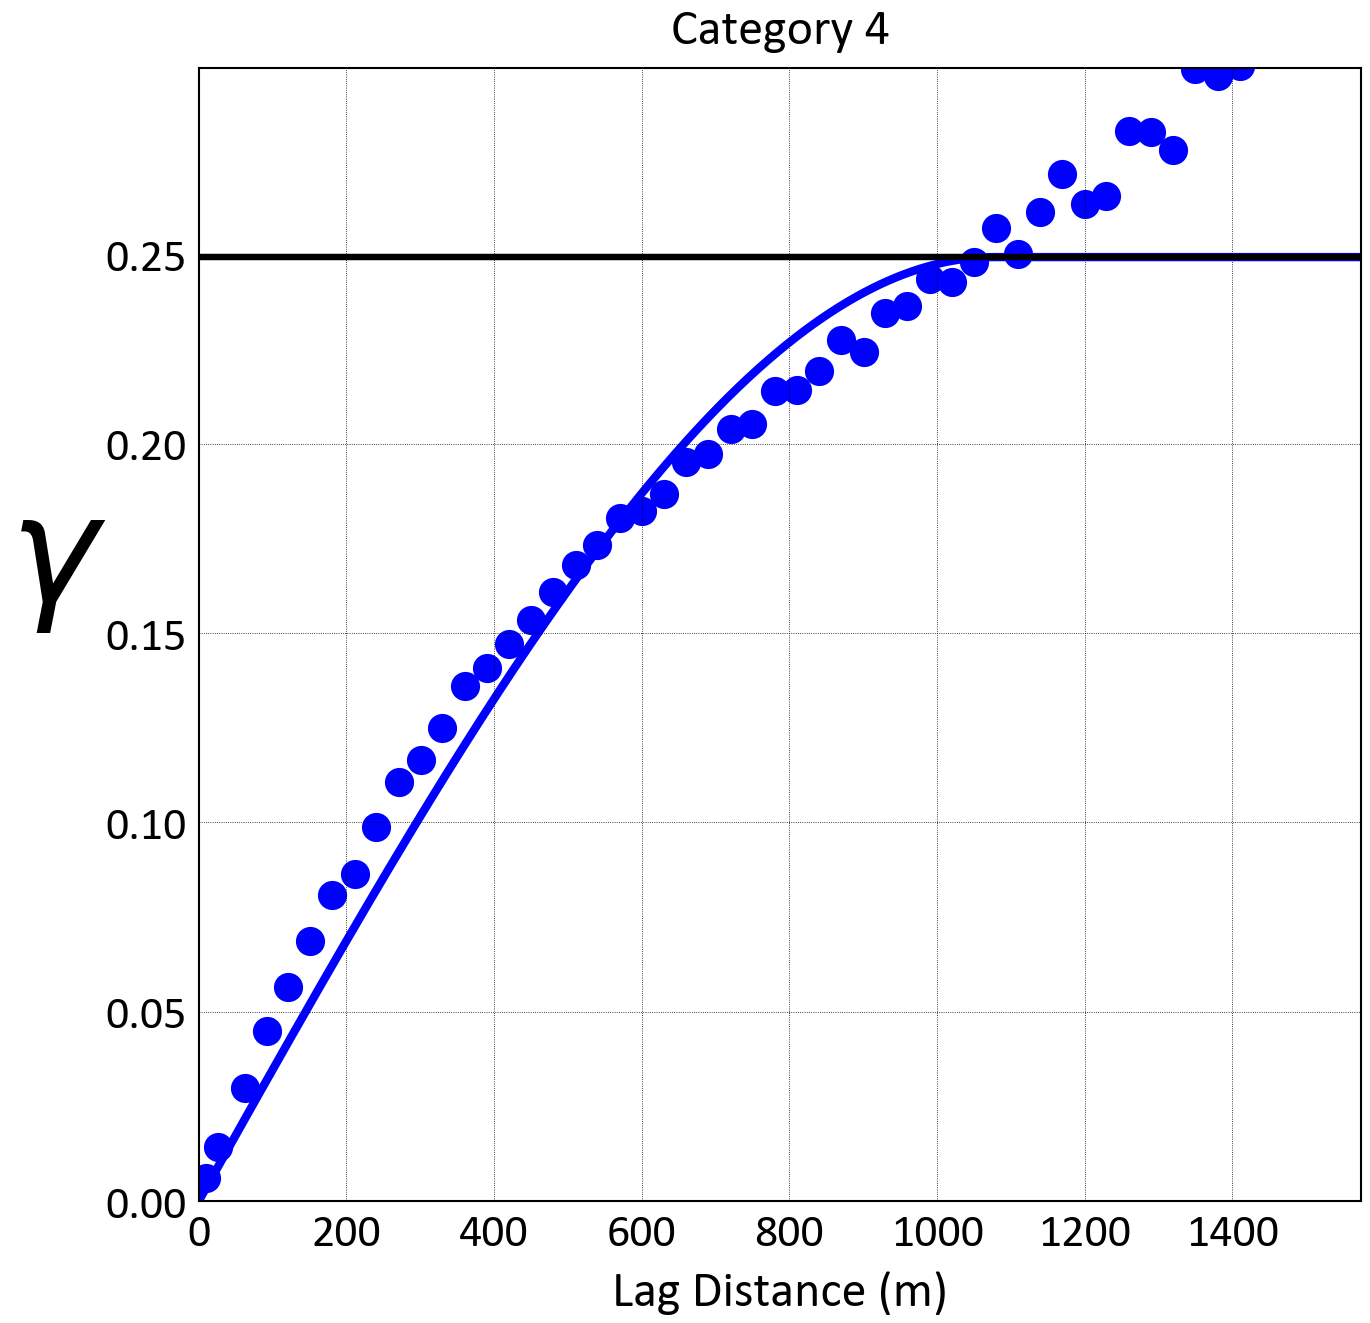
\includegraphics[height=150pt]{capitulo_3/imagens/var_4.png}\label{fig:v4}} \\
    \subfloat[][Variograma omnidirecional para a categoria 5.]{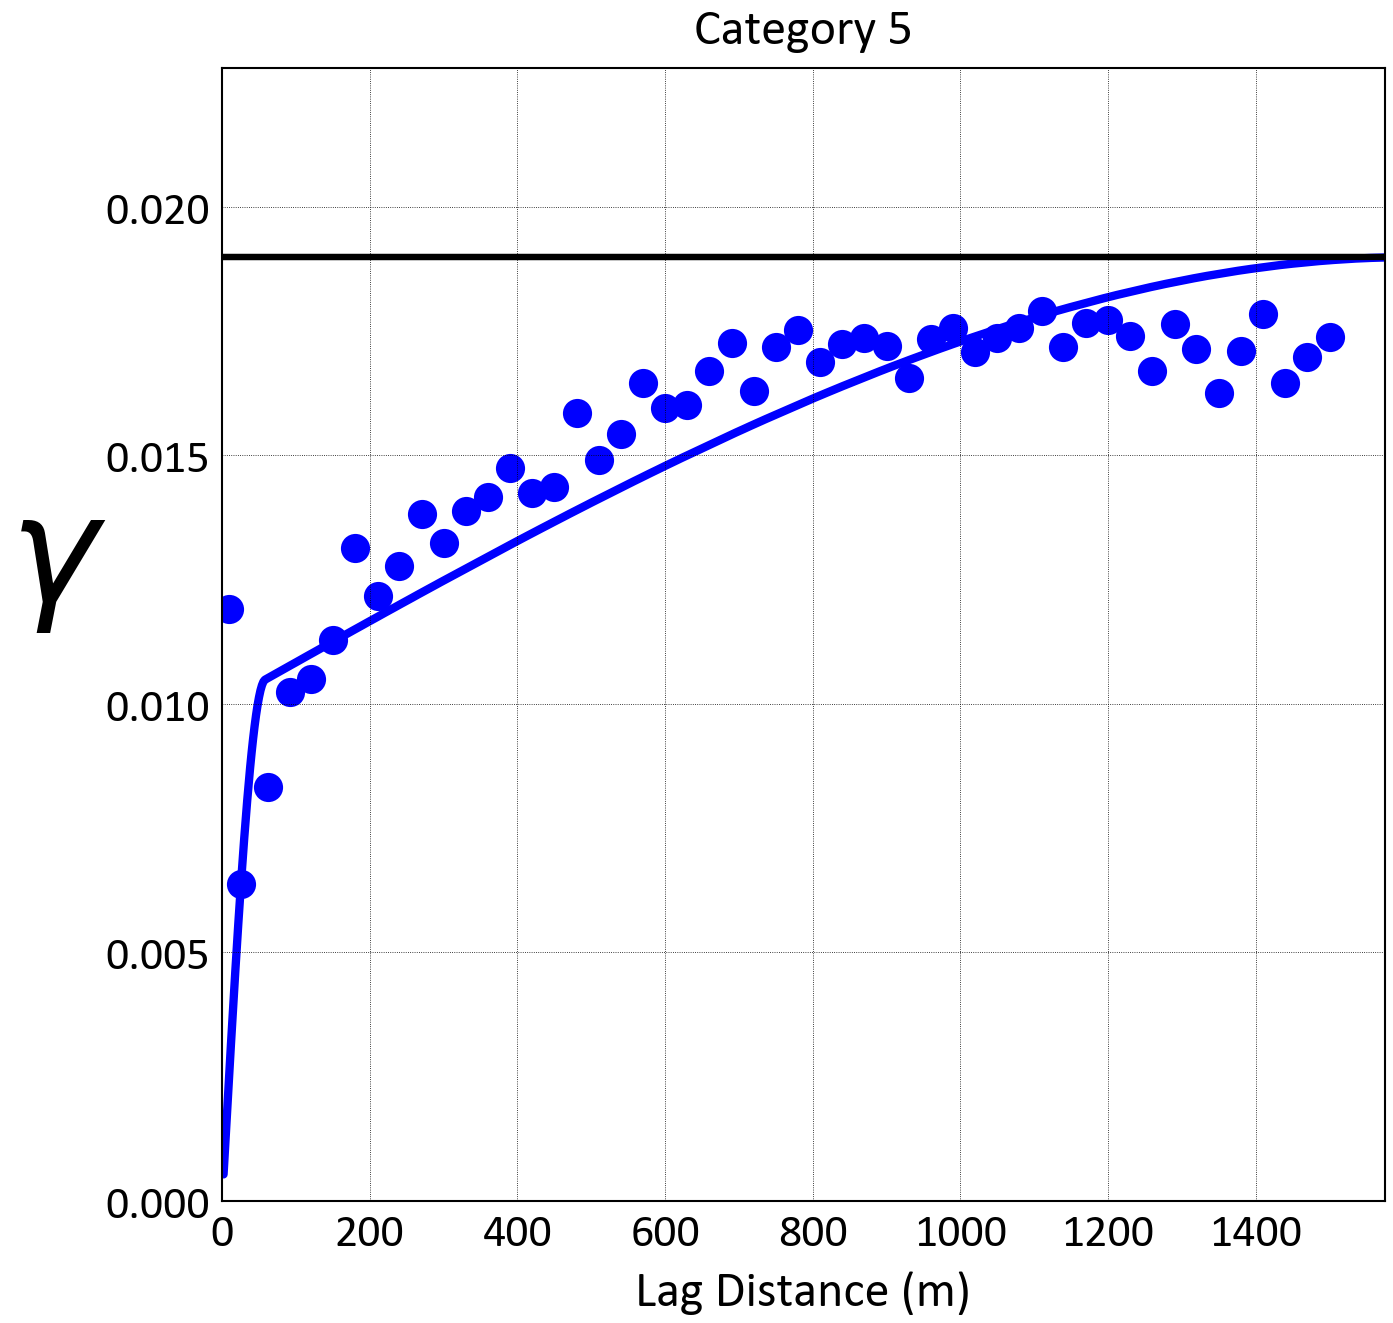
\includegraphics[height=150pt]{capitulo_3/imagens/var_5.png}\label{fig:v5}}
\end{figure}

As distâncias assinaladas calculadas foram interpoladas, por krigagem dual, para um \textit{grid} de 50x50x25 metros usando um equivalente gaussiano para os variogramas dos indicadores ajustados com modelos esféricos (por exemplo, mesmas contribuições, intervalos e razões de anisotropia). Essas dimensões foram escolhidas para o \textit{grid} porque a interpolação dos teores de ouro e posterior planejamento mineiro são feitos, também, nesse \textit{grid}.

Uma largura de 80 metros foi escolhida para a zona de incerteza com base no tipo de depósito e na configuração geométrica amostral. Blocos fora da zona de incerteza foram classificados com a categoria responsável pela distância estimada mais negativas, enquanto blocos dentro da zona de incerteza foram simulados.

Dez realizações de uma simulação não condicional Gaussiana foram realizadas, dentro da zona de incerteza, usando um variograma Gaussiano com um alcance de 600 metros e um pequeno (0,01\%) efeito pepita para evitar instabilidades matemáticas. As realizações foram transformadas em campos de probabilidade e usadas para amostrar uma categoria das distribuições de probabilidade locais. As probabilidades locais foram calculadas transformando as distâncias estimadas dentro da zona de incerteza em probabilidades. A distância máxima estimada absoluta foi usada como o parâmetro $\omega$ para cada bloco, dessa forma, a magnitude da incerteza foi controlada apenas pela largura de zona de incerteza. A \autoref{ouro_reals} mostra uma vista em perspectiva de duas das 10 realizações para o modelo geológico juntamente com as amostras em suporte pontual.

\begin{figure}[H]
	\caption{\label{ouro_reals} Visão em perspectiva de duas das dez realizações juntamente com as amostras em suporte pontual.}
	\centering
		\subfloat[][Realização 1]{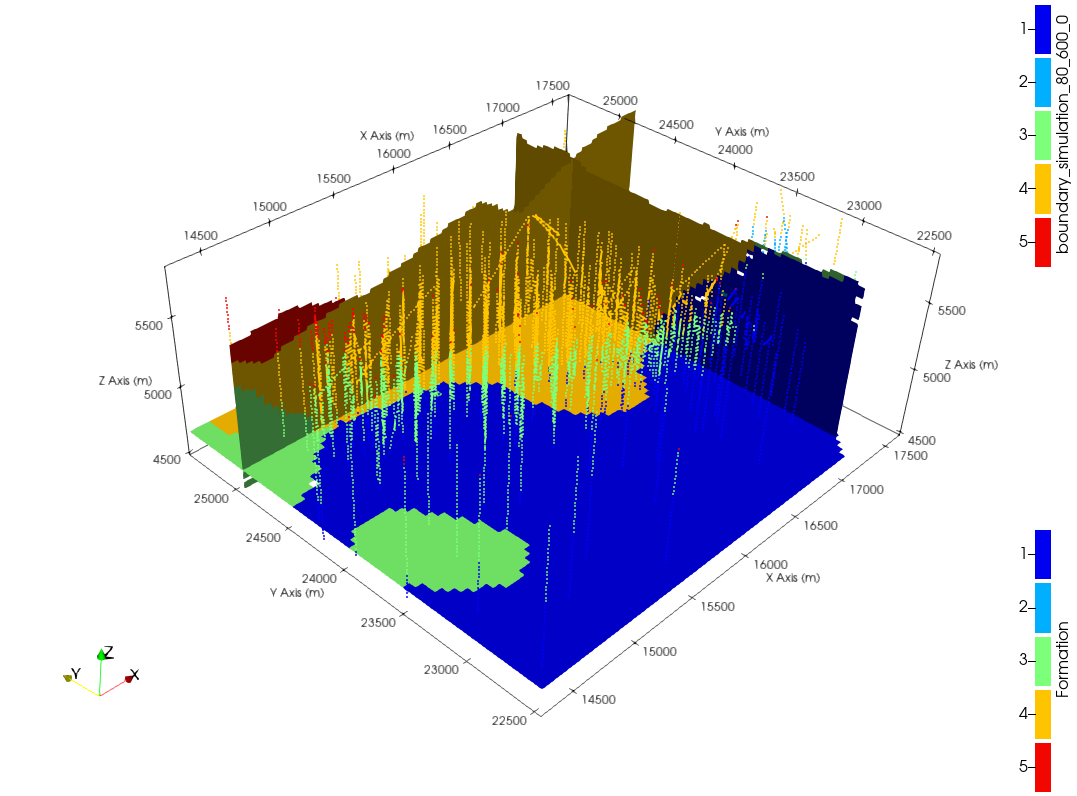
\includegraphics[width=0.45\textwidth]{capitulo_3/imagens/real1.png}\label{fig:g1}}
     \hspace{1em}
     \subfloat[][Realização 2]{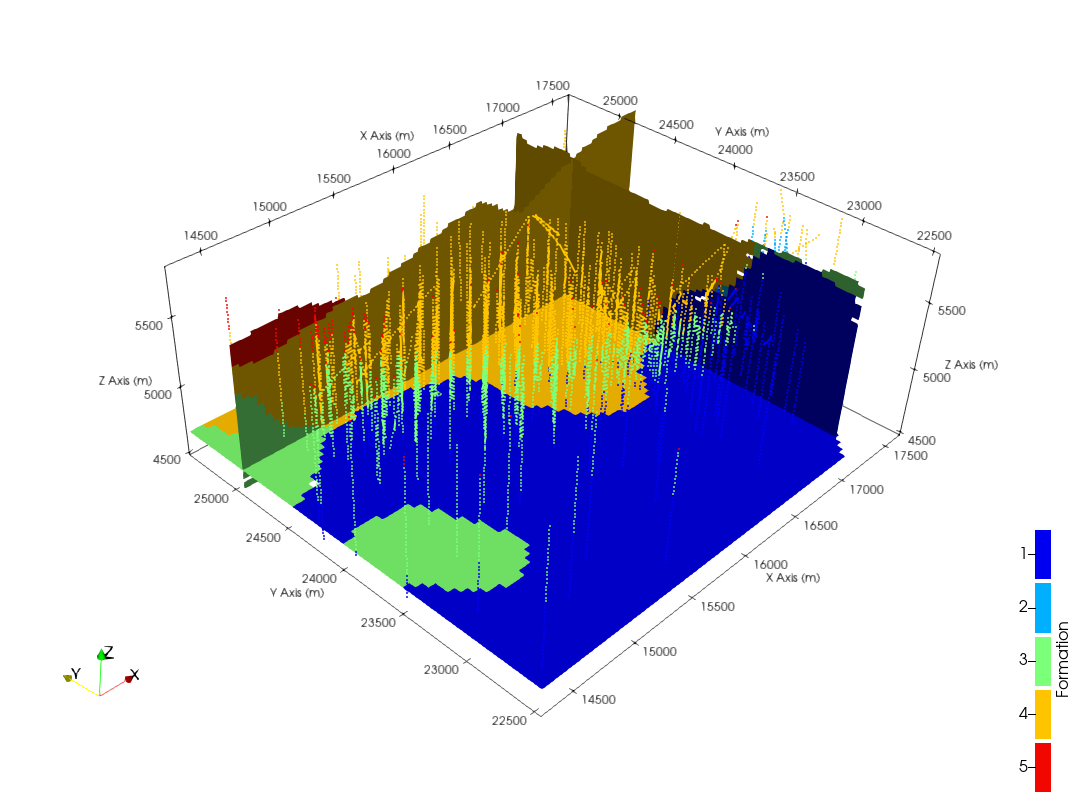
\includegraphics[width=0.45\textwidth]{capitulo_3/imagens/real2.png}\label{fig:g2}}
\end{figure}

\subsection{Discussão}

Uma das técnicas tradicionalmente usadas para modelar geocorpos e avaliar sua incerteza na presença de várias categorias é a simulação sequencial dos indicadores (SISIM). A SISIM foi aplicada ao mesmo banco de dados a fim de comparar os resultados com a metodologia proposta, uma vez que também depende apenas das coordenadas x, y e z dos compósitos e da propriedade categórica. 

A \autoref{sec_comp} mostra um comparativo de seções verticais xz entre a metodologia proposta (\autoref{fig:explicit}), a SISIM (\autoref{fig:sisim}) utilizando o variograma dos indicadores mostrados na \autoref{ouro_vargs}, e um modelo explícito (\autoref{fig:explicit}) elaborado por um geomodelador experiente. Uma animação mostrando as mesmas seções para todas as dez realizações pode ser vista \href{https://github.com/robertorolo/assessing_geological_model_uncertainty_with_probability_fields/blob/main/ezgif-2-802d466feae1.gif}{aqui}. A SISIM gera realizações com uma textura típica \textit{"salt and pepper"} e padrões ruidosos, o que não é geologicamente realista. Enquanto a metodologia proposta cria limites contínuos que são mais semelhantes à interpretação do geomodelador. A ausência de dados de sondagem é responsável pelas regiões onde a metodologia proposta e o SISIM divergem da interpretação do geomodelador.


\begin{figure}[H]
    \caption{Comparativo de seções verticais xz entre a metodologia proposta, a SISIM e um modelo explícito.} \label{sec_comp}
     \centering
     \subfloat[][Modelo explícito.]{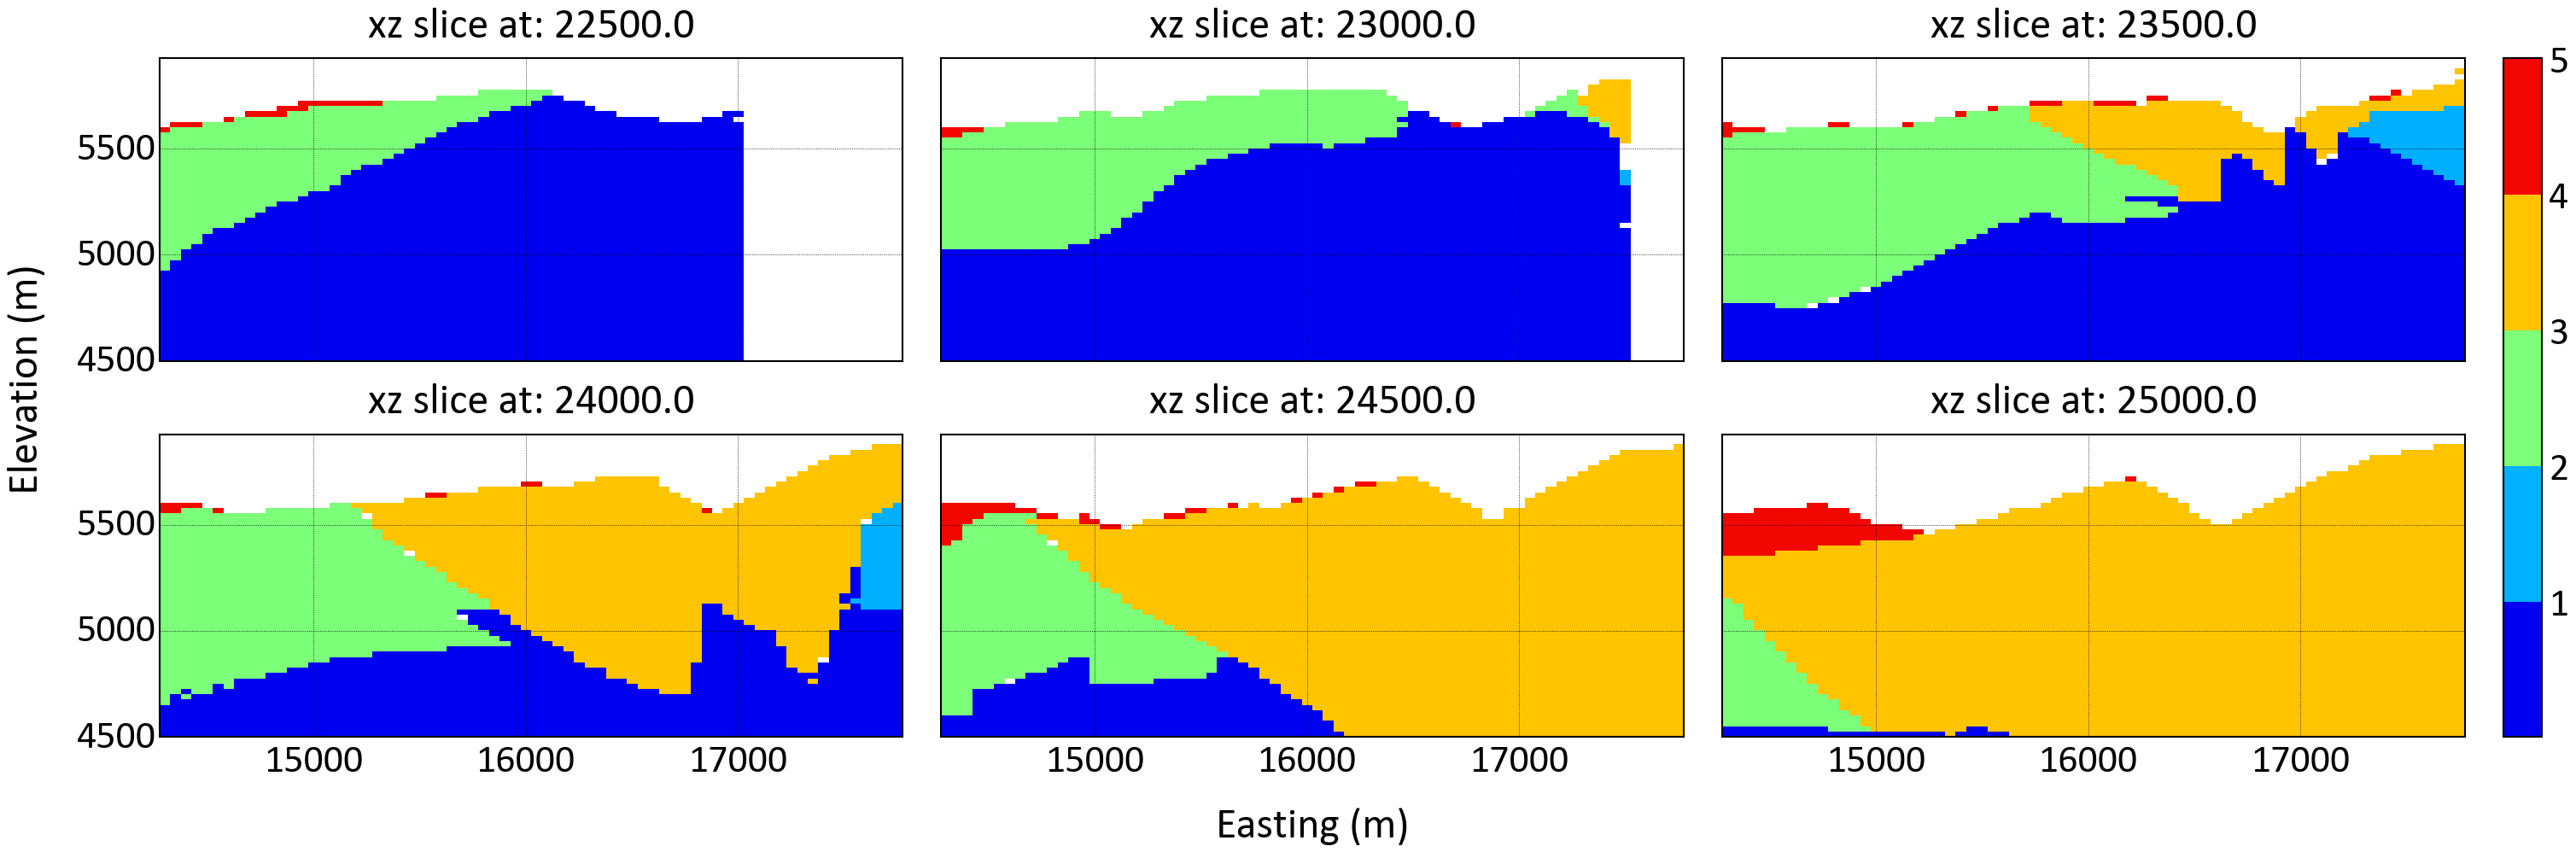
\includegraphics[width=0.8\textwidth]{capitulo_3/imagens/explicit_slicces.png}\label{fig:explicit}}
     \\
     \subfloat[][Metodologia proposta.]{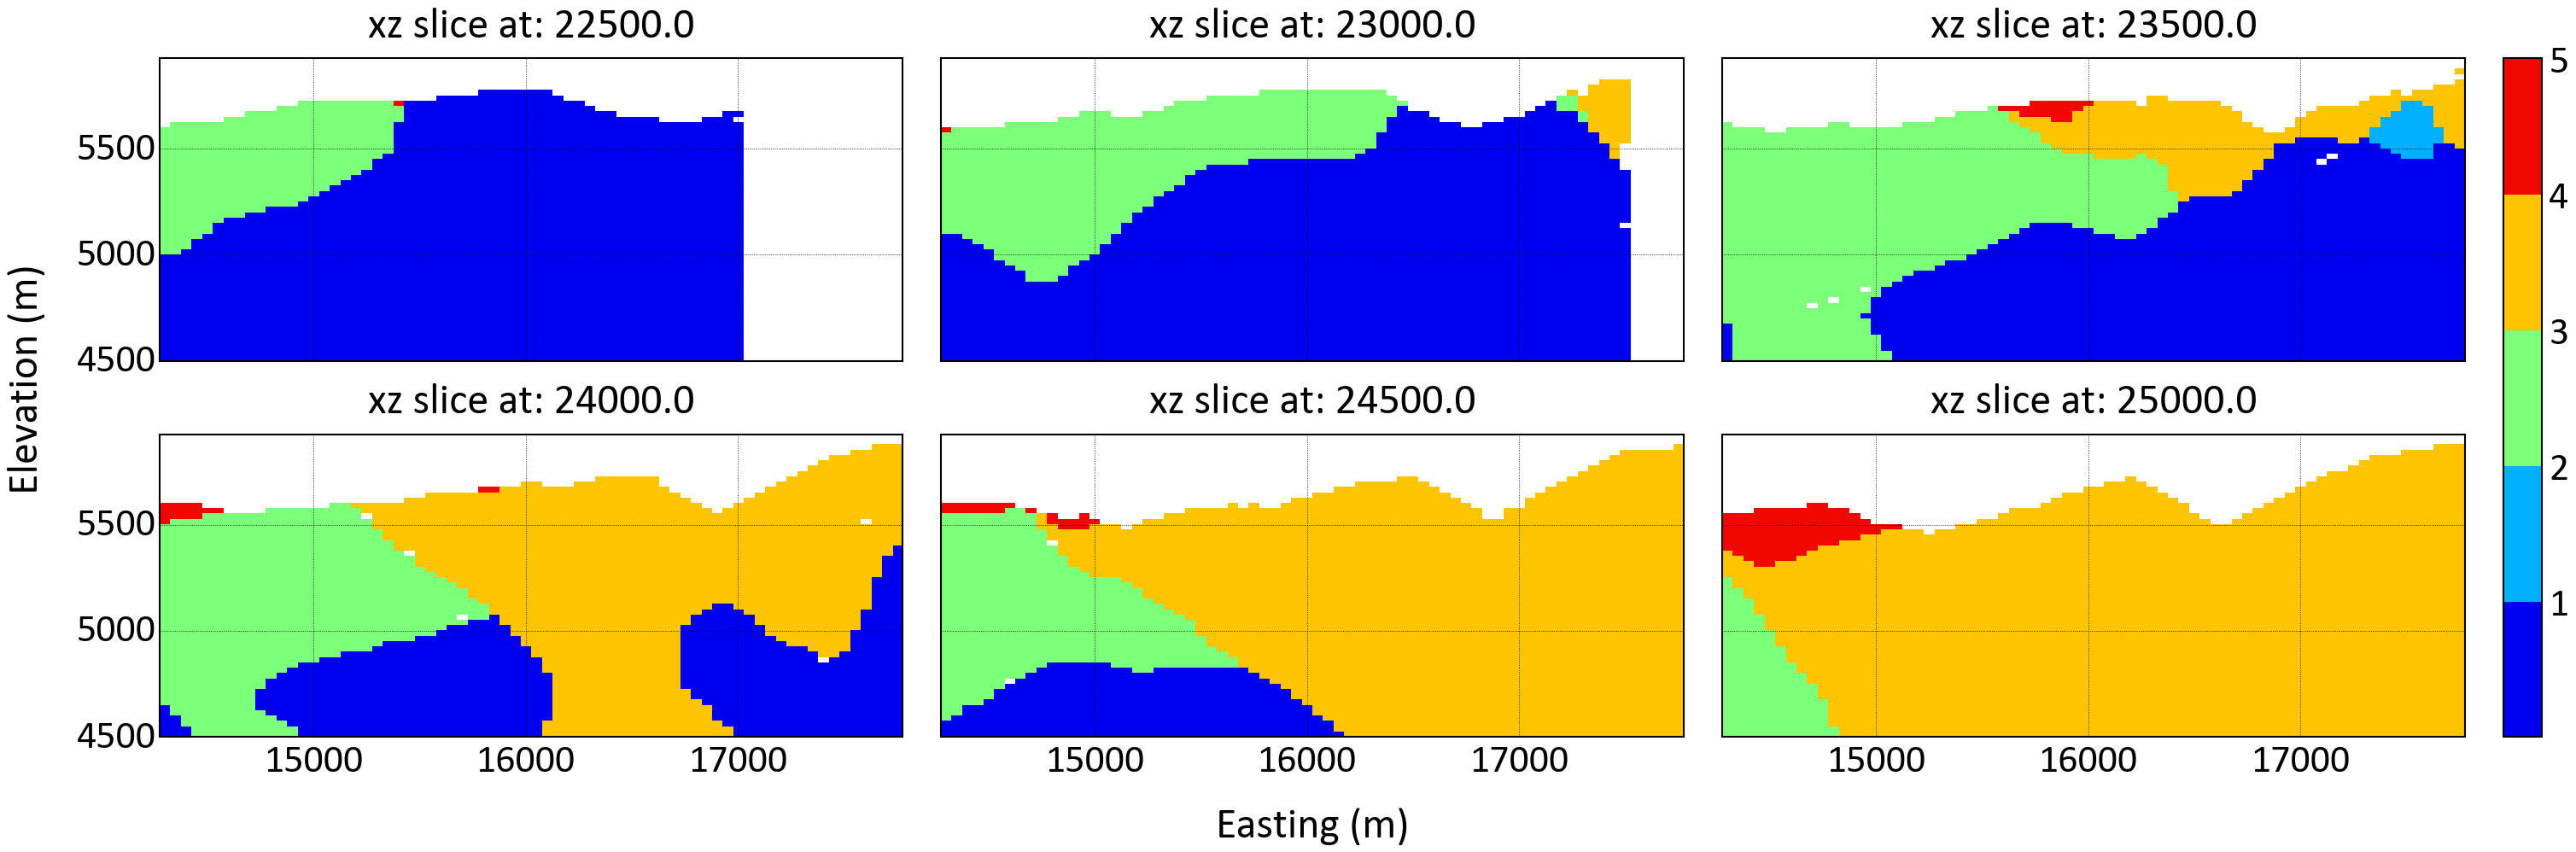
\includegraphics[width=0.8\textwidth]{capitulo_3/imagens/pfields_real_0.png}\label{fig:pfields}}
     \\
     \subfloat[][SISIM.]{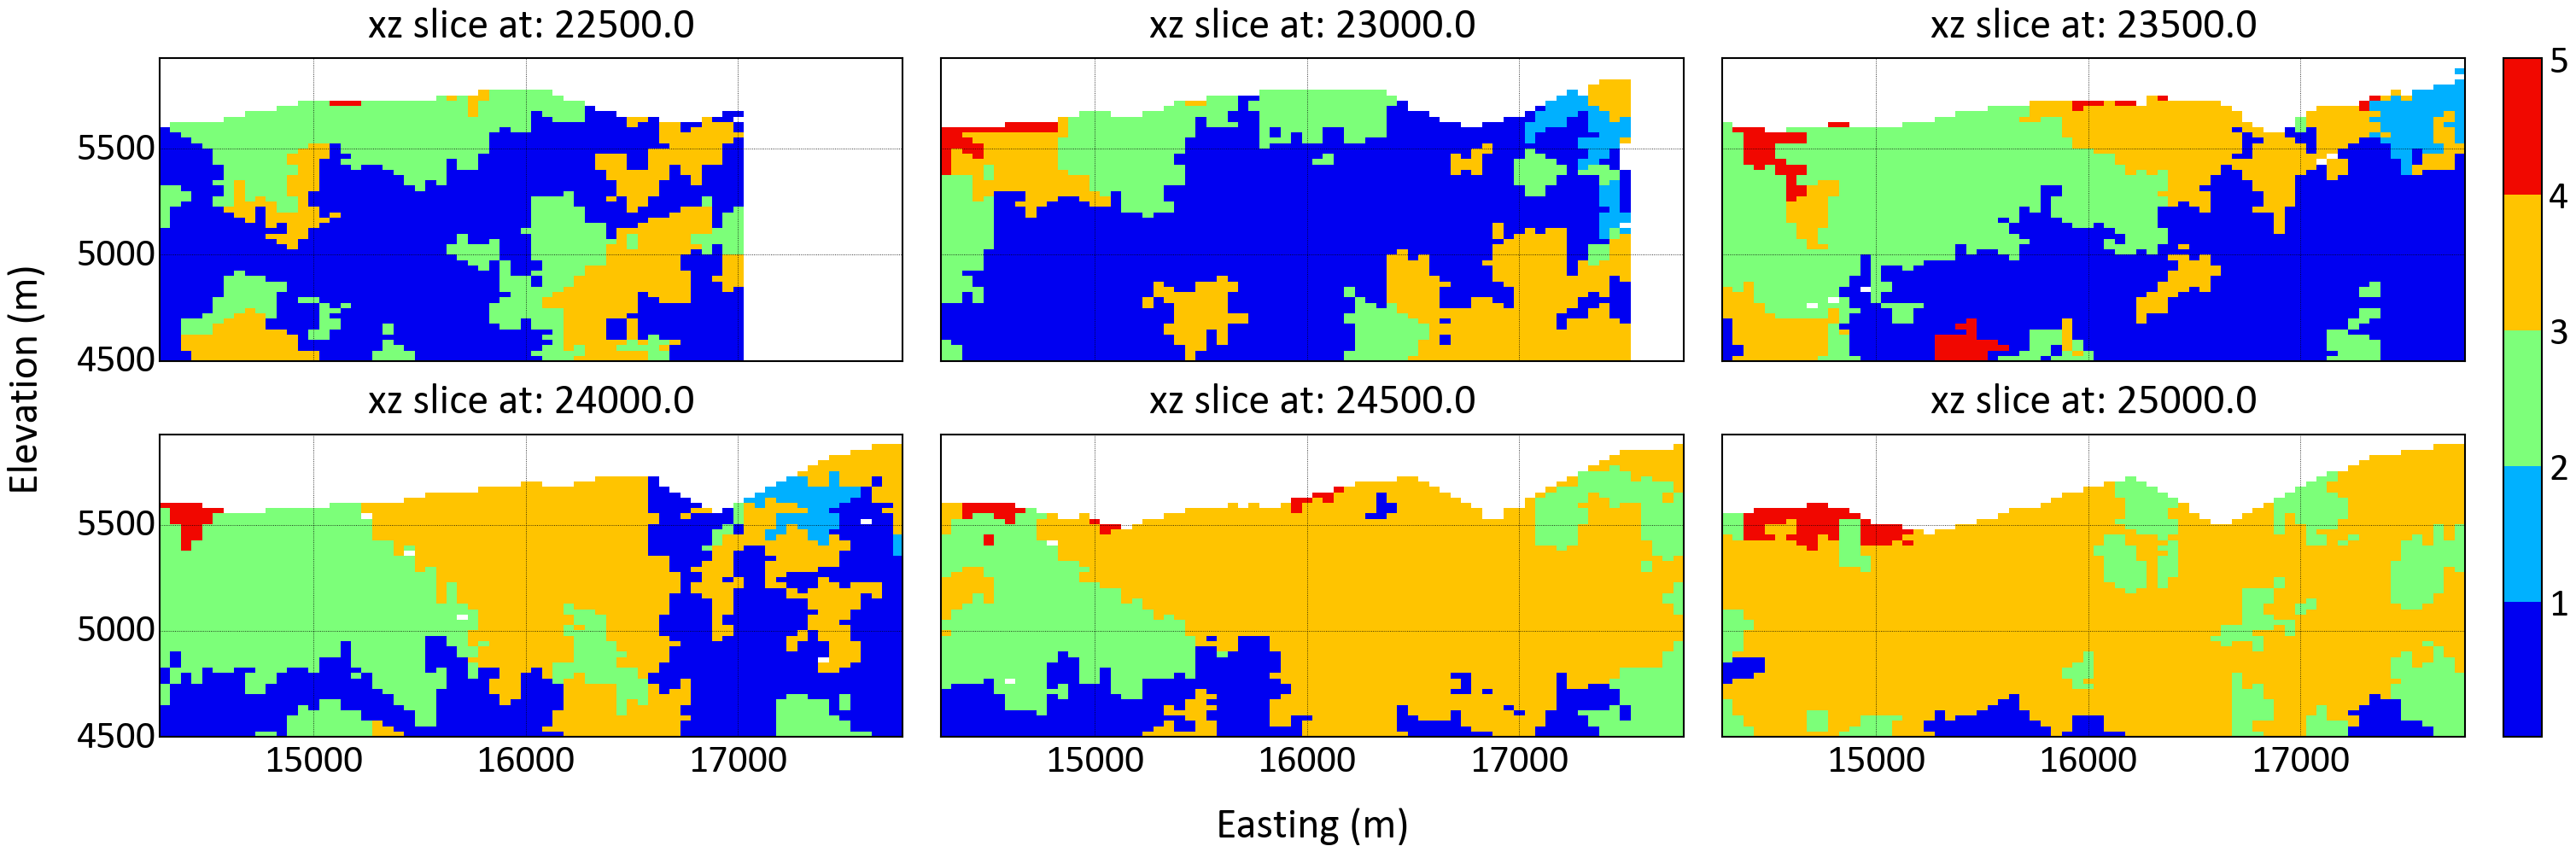
\includegraphics[width=0.8\textwidth]{capitulo_3/imagens/sisim_real_0.png}\label{fig:sisim}}
\end{figure}

O comportamento dos contatos é controlado pelo variograma usado na simulação não condicional; alcances menores e efeitos pepita maiores geram limites irregulares e descontínuos. Por outro lado, longos alcances e pequenos efeitos pepita geram limites suaves e contínuos. A \autoref{sph_jura} mostra uma realização para o \textit{Swiss Jura} criada usando um variograma esférico com um alcance de 50 metros. Os contatos são mais ásperos do que aqueles vistos na \autoref{reals_pfield_jura}, que foram gerados por um variograma Gaussiano.

\begin{figure}[H]
	\caption{\label{sph_jura} Uma realização para o \textit{Swiss Jura} criada usando um variograma esférico para a simulação não condicional.}
	\centering
		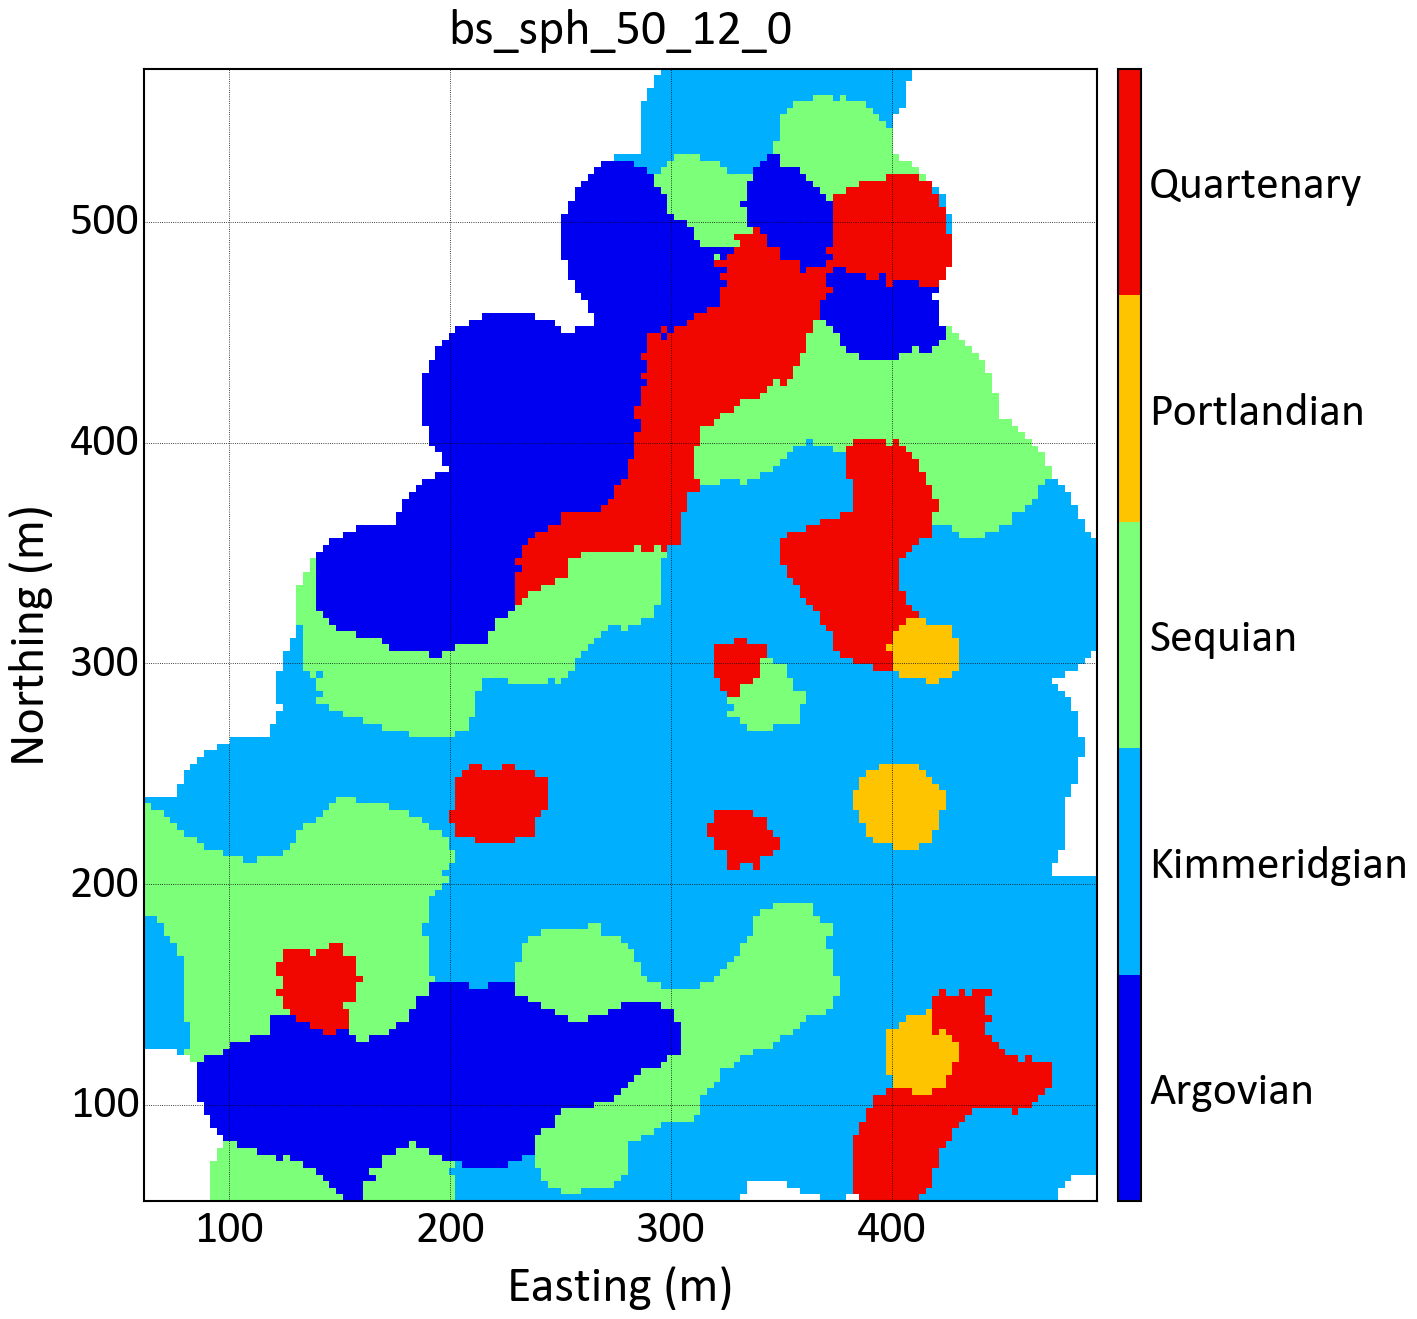
\includegraphics[width=0.6\textwidth]{capitulo_3/imagens/sph_real_0_50_12.png}
\end{figure}

A magnitude da incerteza é controlada tanto pela largura de zona de incerteza quanto pelo parâmetro $\omega$. Uma animação mostrando 10 realizações feitas para o \textit{Swiss Jura} com o mesmo variograma Gaussiano, entretanto, para uma largura da zona de incerteza de 20 metros pode ser vista \href{https://github.com/robertorolo/assessing_geological_model_uncertainty_with_probability_fields/blob/main/ezgif-2-721b458d5c70.gif}{aqui}. Como há mais área para os contatos mudarem de posição, a variação de área é maior do que a observada para a largura de banda de 12 metros. O mesmo comportamento é evidenciado pelos mapa de entropia calculados a partir da \autoref{shannon_entr} (e estandardizadas para que os valores estejam entre 0 e 1) para as bandas de incerteza de 12 e 20 metros.

\begin{figure}[H] 
    \centering
    \caption{Entropia calculada a partir das dez realizações no \textit{Swiss Jura}.} \label{jura_entropy}
     \subfloat[][Zona de incerteza de 12 metros.]{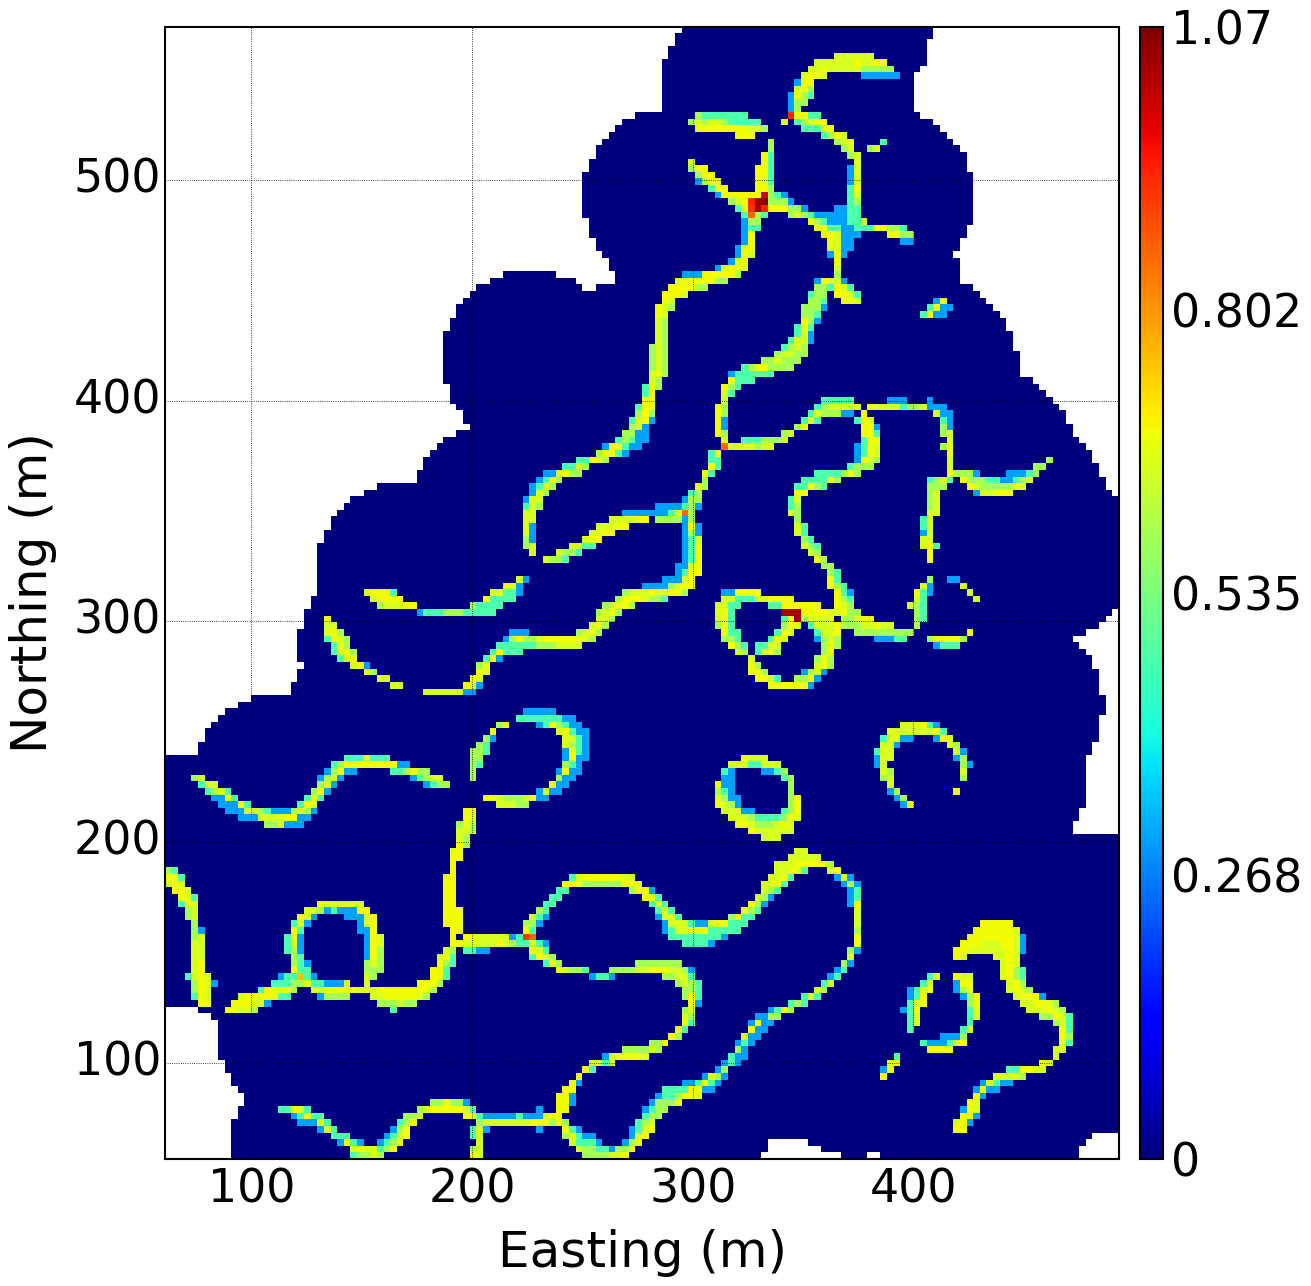
\includegraphics[width=.45\textwidth]{capitulo_3/imagens/jura_entropy_12.png}\label{<figure1>}}
     \hspace{1em}
     \subfloat[][Zona de incerteza de 20 metros.]{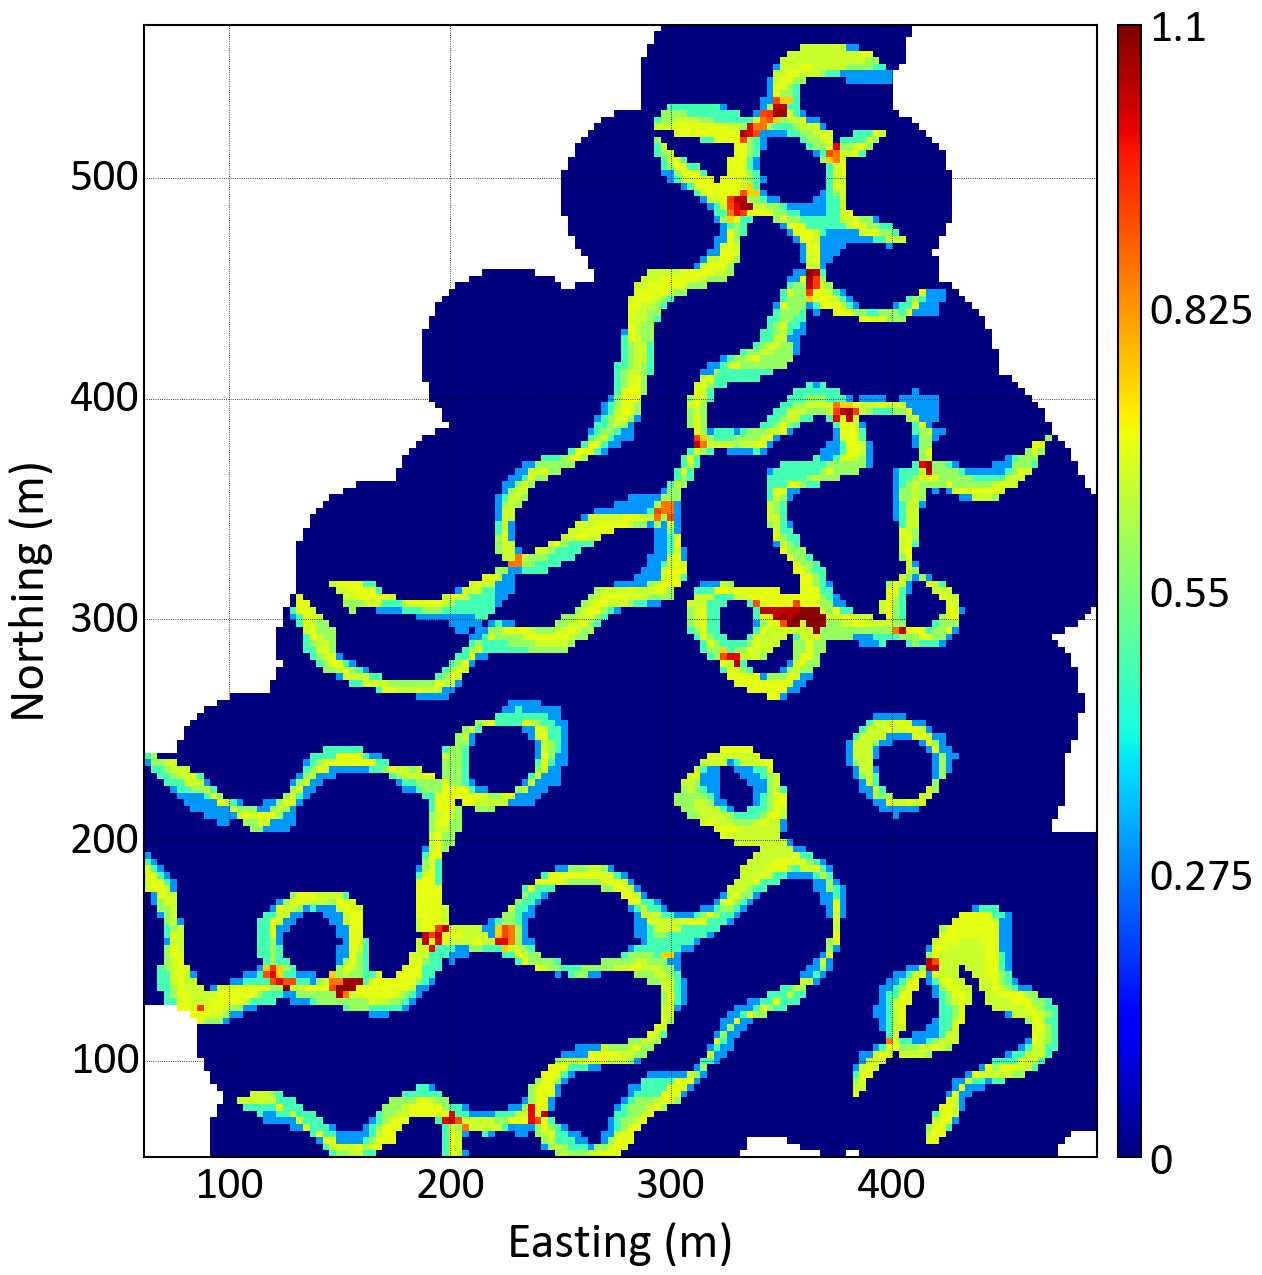
\includegraphics[width=.45\textwidth]{capitulo_3/imagens/jura_entropy_20.png}\label{<figure2>}}
\end{figure}

A \autoref{areas_jura} mostra a área para as categorias Swiss Jura para 10 realizações com larguras de banda de 12 e 20 metros. Os desvios padrão das áreas também são mostrados. O gráfico mostra que as áreas têm maior variação para todas as categorias quando a largura de banda da incerteza é de 20 metros.

\begin{figure}[H]
	\caption{\label{areas_jura} Variação de volume para todas as categorias do \textit{Swiss Jura} para 10 realizações com larguras de banda de 12 e 20 metros.}
	\centering
		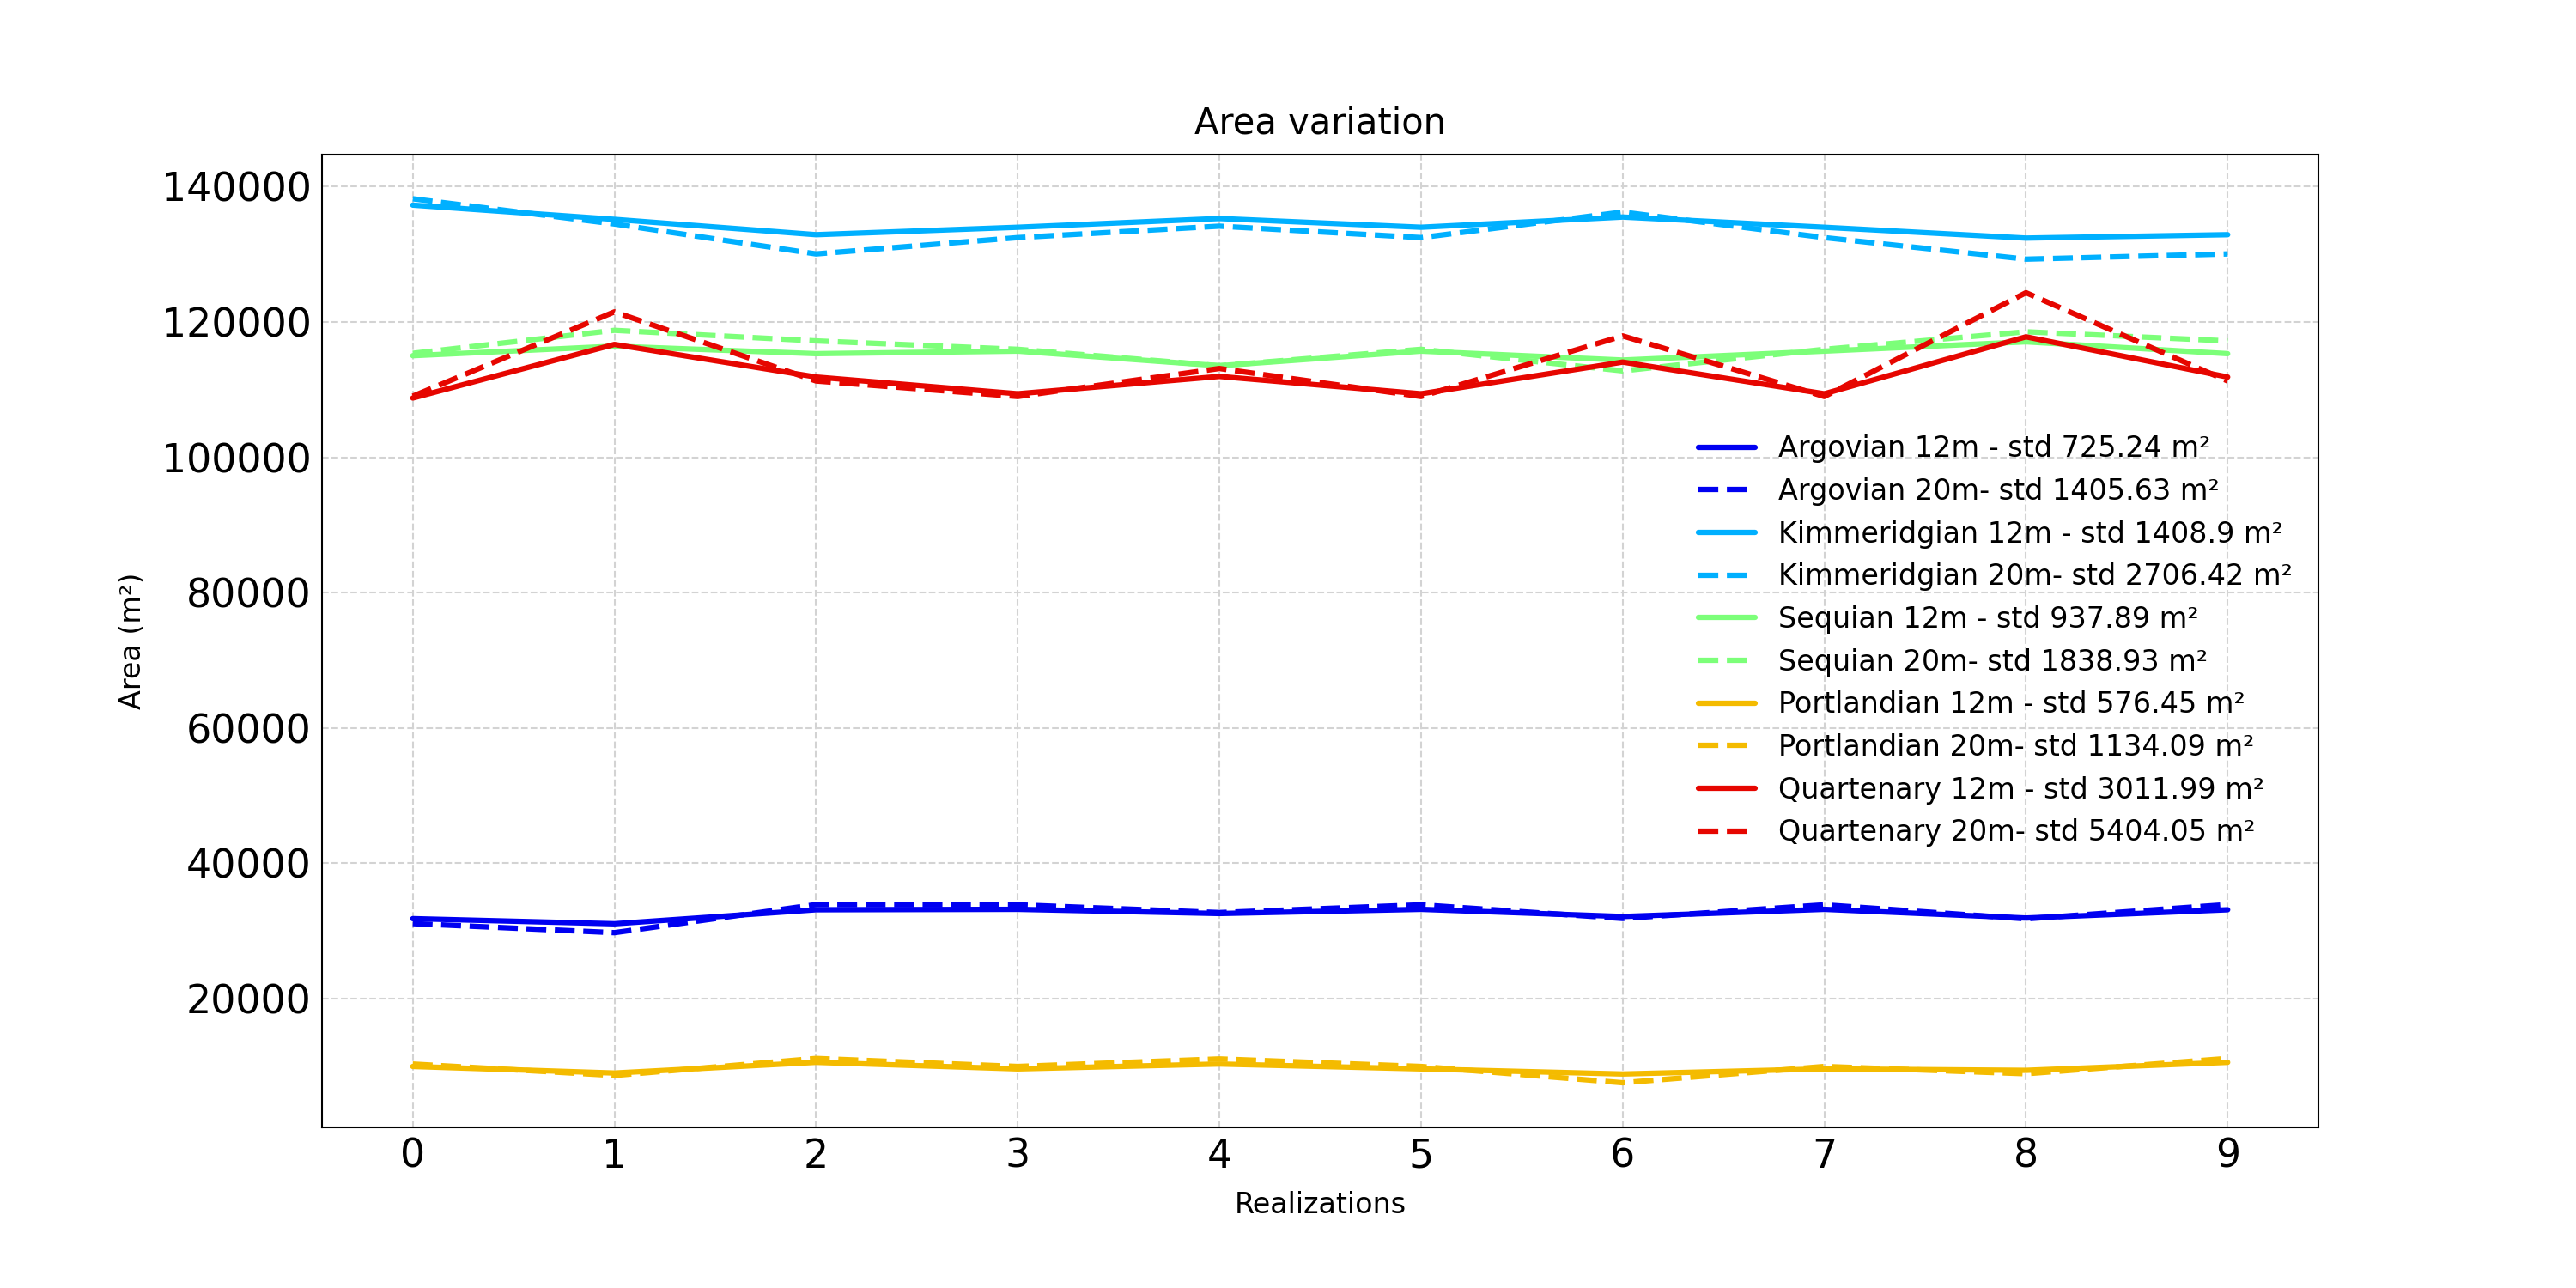
\includegraphics[width=\textwidth]{capitulo_3/imagens/areasjura.png}
\end{figure}

A \autoref{conf_mat_pfields} mostra uma matriz de confusão representando a média da proporção de blocos que reproduzem as amostras mais próximas entre todas as realizações, para todas as categorias no banco de dados. A reprodução é alta para categorias de alto volume com abundância de amostras. As categorias 2 e 5 têm menos volume e menos amostras em comparação com as categorias 1, 3 e 4, o que explica a menor reprodução. Para a categoria 5, o problema é acentuado, uma vez que existem apenas algumas amostras esparsas na superfície do depósito. A distância estimada das categorias de volume mais altas sempre será mais negativa nesses casos. Uma maneira de contornar esse problema é pré-processar os modelos atribuindo as categorias de amostra aos blocos mais próximos. Esta solução congelaria alguns blocos com base no valor da amostra mais próxima, minimizando o desvanecimento dessas categorias em relação à se fossem interpoladas/simuladas com dados circundantes.

\begin{figure}[H]
	\caption{\label{conf_mat_pfields} Matriz de confusão mostrando a média da proporção de blocos que reproduzem as amostras mais próximas entre todas as realizações para todas as categorias do banco de dados.}
	\centering
		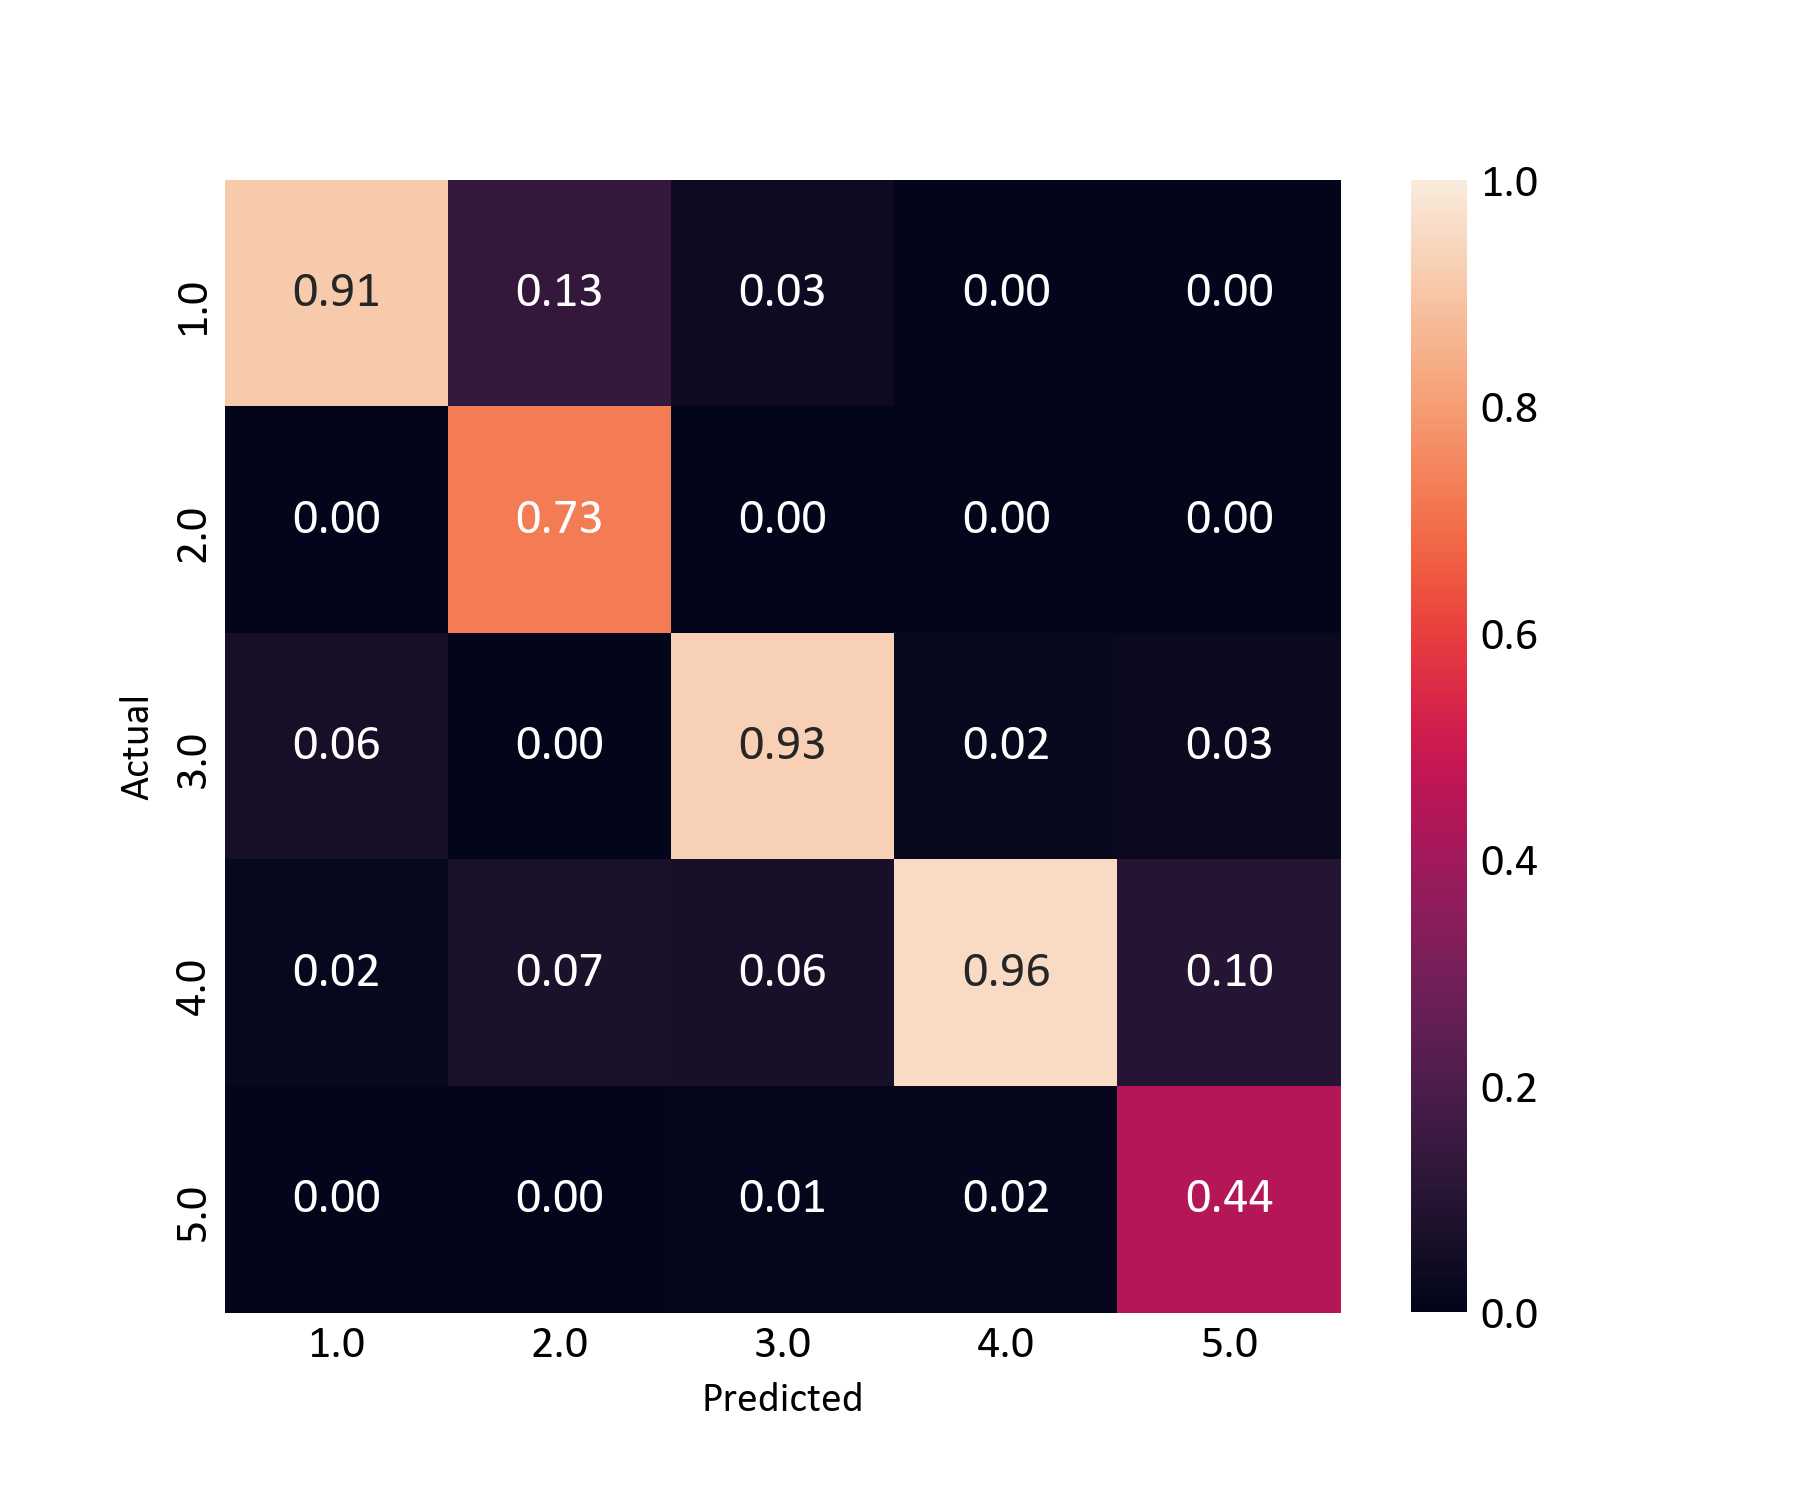
\includegraphics[width=0.6\textwidth]{capitulo_3/imagens/backflag.png}
\end{figure}

\section{Simulação hierárquica dos contatos}

A proposta dessa metodologia é avaliar a incerteza do modelo geológico multi-categórico simulando os contatos entre os diferentes domínios com base no método proposto por \citeonline{wilde2012kriging} a partir dos furos de sondagem compositados, apresentando coordenadas X, Y e Z e propriedade categórica que representa as diferentes litologias. O método de \citeonline{wilde2012kriging} funciona apenas para casos binários e fazer sua aplicação ingenuamente em casos de múltiplos domínios é demorado, subjetivo e pode causar sobreposição de blocos atribuídos à diferentes categorias em diferentes realizações ou produzir blocos não atribuídos à nenhuma categoria em algumas das realizações. Por esse motivo essa tese propõe um algoritmo para agrupar automaticamente as diferentes litologias e um fluxo de trabalho para simular cada grupo individualmente e, em seguida, reconstruir o modelo geológico multi-categórico, a partir do agrupamento, de forma hierárquica. 

A metodologia foi inicialmente proposta por \citeonline{amarante_incerteza_associada} e foi posteriormente aprimorada tendo sua subjetividade reduzida e automatização aumentada \cite{amarante2021boundary}. Um outro estudo de caso foi conduzido em um banco de dados de ferro por \citeonline{amarante2019assessing} e o método se mostrou competente, apresentando resultados melhores em relação a outros métodos concorrentes.

A primeira etapa do fluxo de trabalho é definir grupos de amostras que representam os contatos entre as diferentes litologias do depósito mineral. O agrupamento pode ser definido explicitamente por um geomodelador ou pode ser feito automaticamente pelo algoritmo proposto.

O algoritmo de cubos marchantes, apresentado na \autoref{bound_ref}, é aplicado a um proto-modelo geológico para identificar e contar os contatos. O proto-modelo pode ser criado pelo vizinho mais próximo, máquina de vetores de suporte, krigagem dos indicadores ou usando funções distâncias assinaladas em um \textit{grid} mais grosseiro do que o \textit{grid} de simulação final para acelerar o processo.

A \autoref{fig:jura_proto} mostra um proto-modelo geológico criado a partir do banco de dados \textit{Swiss Jura} usando distâncias assinaladas em um \textit{grid} de 10x10 metros. A resolução do \textit{grid} pode alterar o agrupamento final.

\begin{figure}[H]
    \caption{Proto-modelo e blocos sinalizados como contatos pelo algoritmo cubos marchantes para o \textit{Swiss Jura}.} \label{fig:jura_proto}
     \centering
     \subfloat[][Proto-modelo geológico]{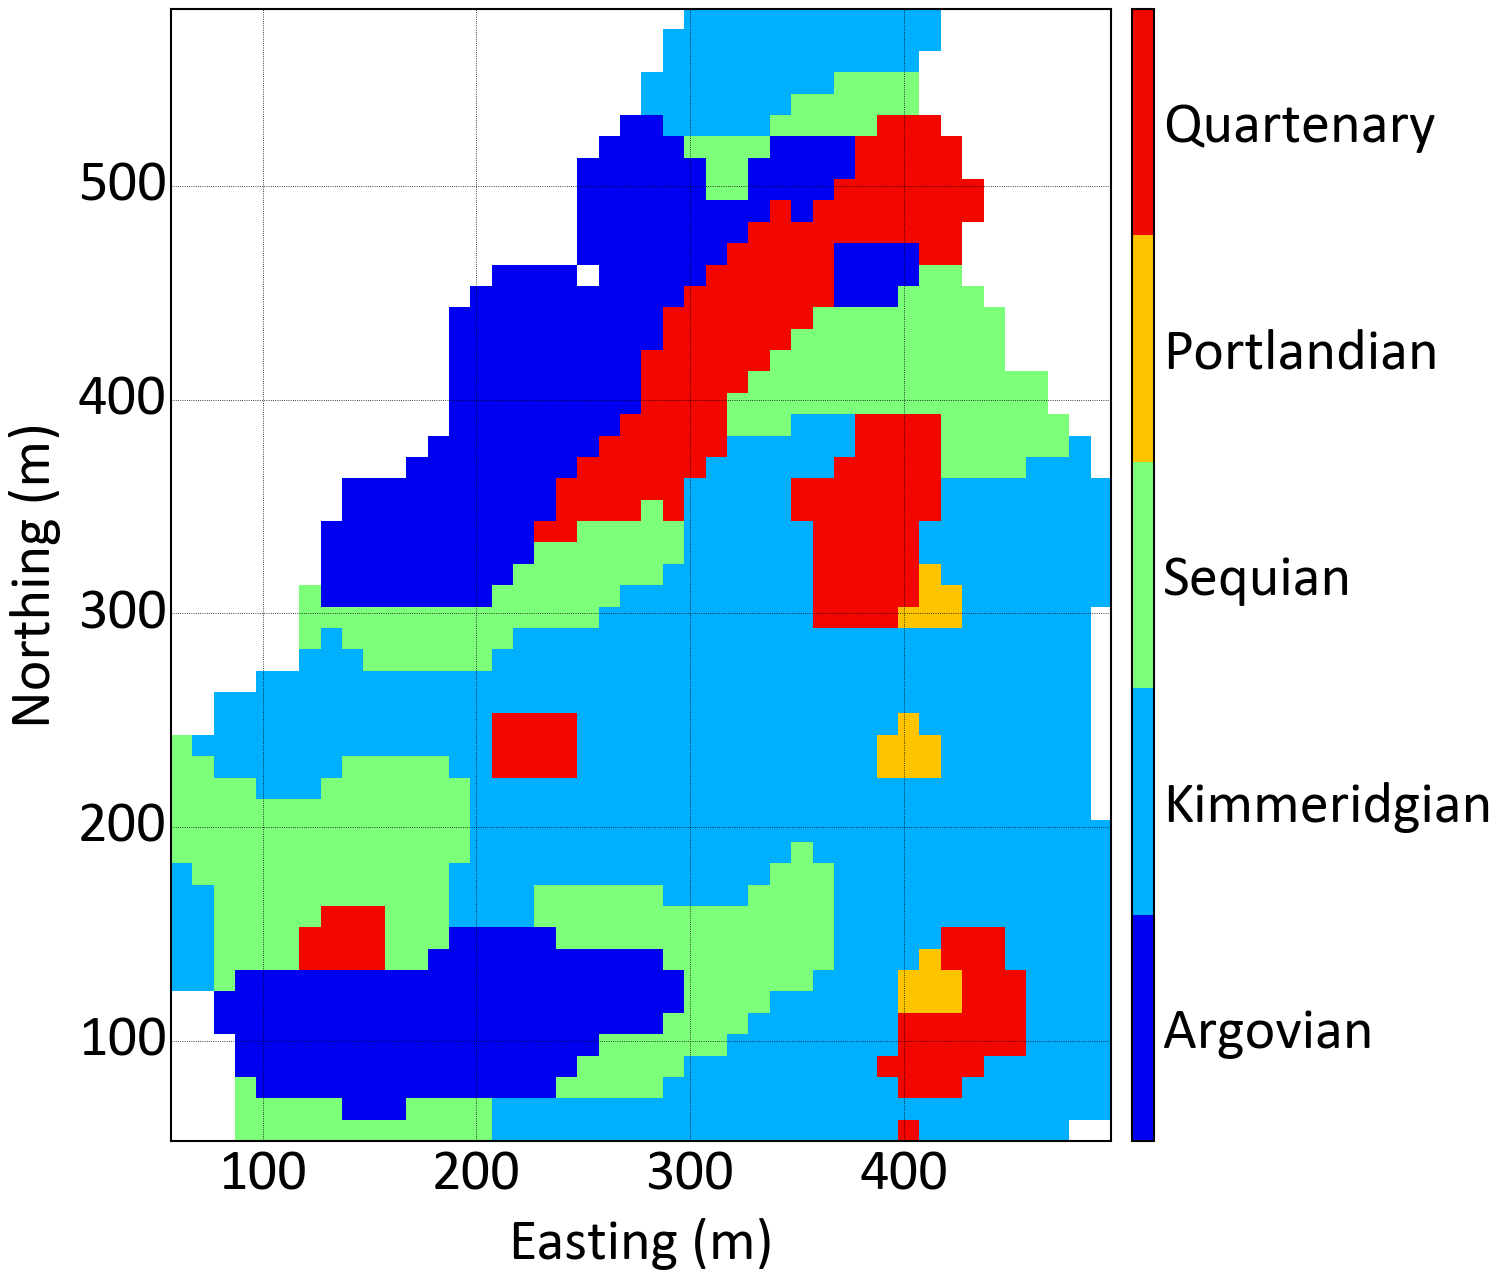
\includegraphics[height=150pt]{capitulo_3/imagens/geomodel.png}\label{fig:proto}}
     \hspace{1em}
     \subfloat[][Blocos sinalizados como contatos. As cores indicam quantas categorias fazem parte desse contato.]{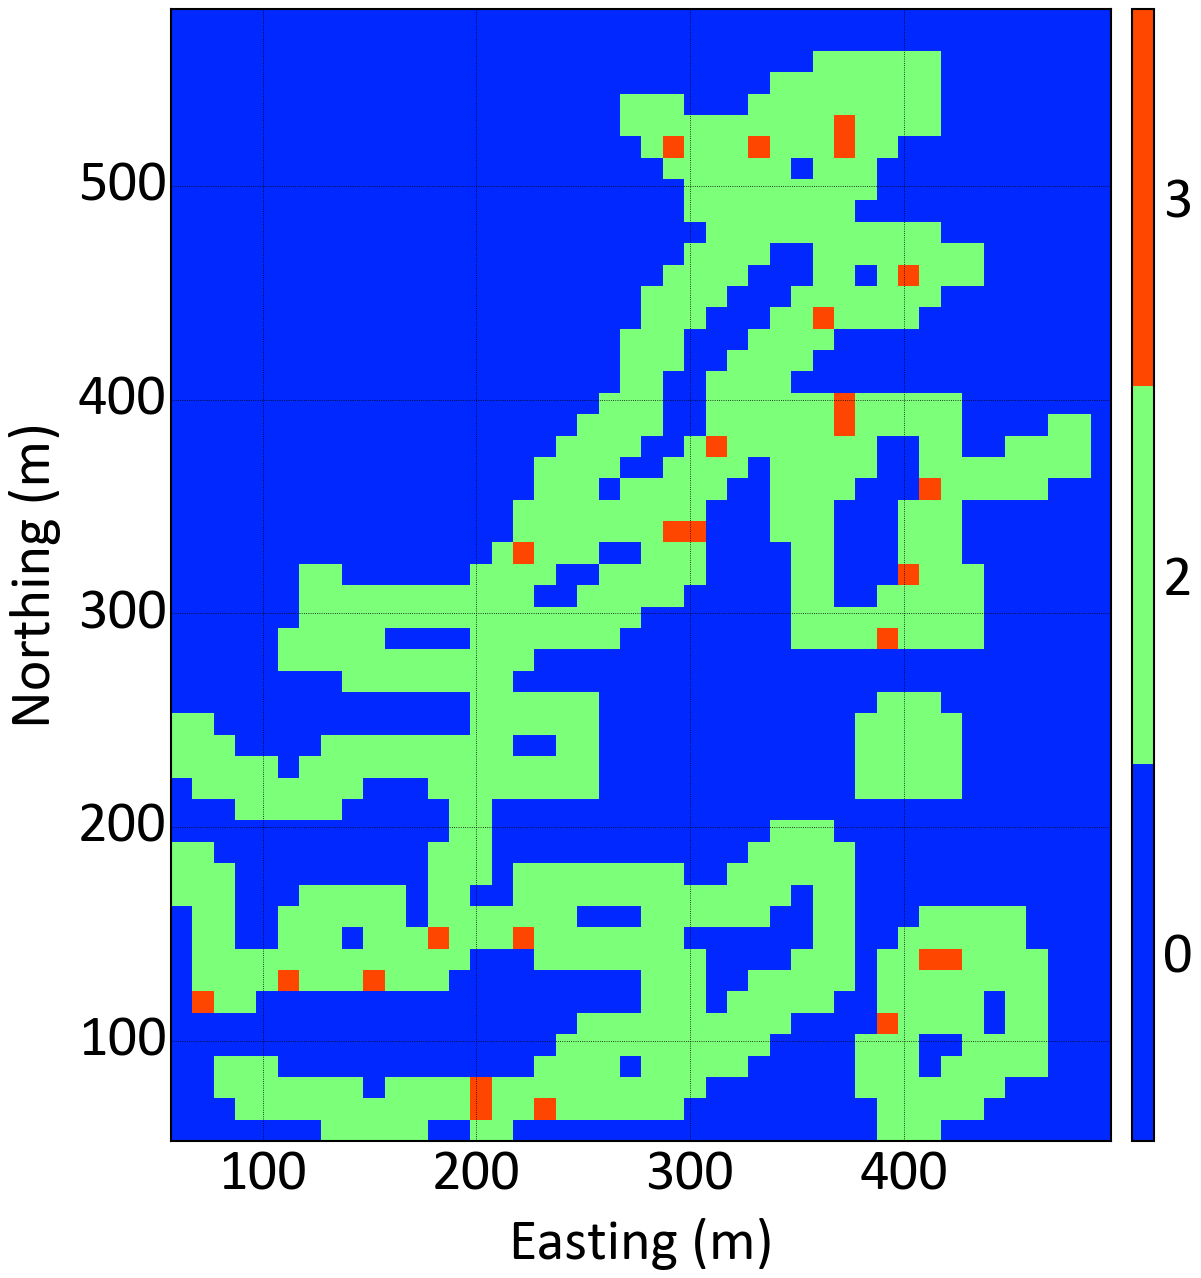
\includegraphics[height=150pt]{capitulo_3/imagens/cdelim.png}\label{fig:contacts}}
\end{figure}

O número de conatatos entre as diferentes litologias, contados pelo algoritmo dos cubos marchante, são mostrados na \autoref{table:contact_count}.

\begin{table}[H]
\caption{Contagem de contatos pelo algoritmo dos cubos marchantes.} \label{table:contact_count}
\centering
\begin{tabular}{|l|l|}
\hline
Kimmeridgian; Sequian                 & 134 \\ \hline
Argovian; Sequian                     & 74  \\ \hline
Kimmeridgian; Quartenary              & 66  \\ \hline
Argovian; Quartenary                  & 45  \\ \hline
Sequian; Quartenary                   & 40  \\ \hline
Kimmeridgian; Portlandian             & 23  \\ \hline
Portlandian; Quartenary               & 9   \\ \hline
Argovian; Kimmeridgian                & 8   \\ \hline
Argovian; Kimmeridgian; Sequian       & 7   \\ \hline
Argovian; Sequian; Quartenary         & 6   \\ \hline
Kimmeridgian; Portlandian; Quartenary & 4   \\ \hline
Kimmeridgian; Sequian; Quartenary     & 4   \\ \hline
\end{tabular}
\end{table}

Para definir os (K-1) grupos, onde K é o número de categorias do conjunto de dados, o Algoritmo \ref{algo:group} é aplicado. Os primeiros grupos representam os contatos mais frequentes. Na iteração inicial, a variável i é o número par 0, o algoritmo irá criar um grupo onde as amostras das categorias Kimmeridgian e Sequian são codificadas como 1 e as amostras de outras categorias são codificadas como 0. Na segunda iteração, a variável i recebe o número ímpar 1, portanto o algoritmo irá criar um grupo onde as amostras da categoria Kimmeridgian são codificadas como 1 e Sequian são codificadas como 0. Além disso, o algoritmo irá remover da tabela de contagem de contatos quaisquer contatos em que Kimmeridgian ou Sequian façam parte, a saber, linhas 1, 2, 3, 5, 6 e 7. A variável i apresenta o valor par igual a 2 na terceira iteração, assim um grupo é criado onde as amostras das categorias Argovian e Quartenary são codificadas como 1 e as outras categorias da tabela de contagem de contatos, após a remoção das de linhas, são codificadas como 0, pois este é o contato mais frequente após a remoção das linhas. O algoritmo assume que os primeiros (K-1) contatos mais frequentes serão entre duas, não mais, categorias, o que é razoável em um contexto geológico.

\begin{algorithm}[H]
\SetAlgoLined
 \For{i in (K-1)}{
  \eIf{i\%2!=0}{
   1. Cria um grupo: categorias do contato mais frequente são codificadas como 1, outras categorias são codificadas como 0\;
   }{
   1. Cria um grupo: uma categoria do contato mais frequente é codificada como 1, a outra como 0\;
   2. Remove da lista de contagem de contatos todos os contatos que contêm pelo menos uma das categorias do contato mais frequente\;
  }
 }
 \caption{Define os grupos a partir da tabela de contagem dos contatos.}\label{algo:group}
\end{algorithm}

A figura \ref{fig:groups_fig} mostra a regra de hierarquia definida pelo algoritmo proposto para o proto-modelo do \textit{Swiss Jura}.

\begin{figure}[H]
	\caption{\label{fig:groups_fig} Regra hierárquica definida pelo algoritmo proposto.}
	\centering
		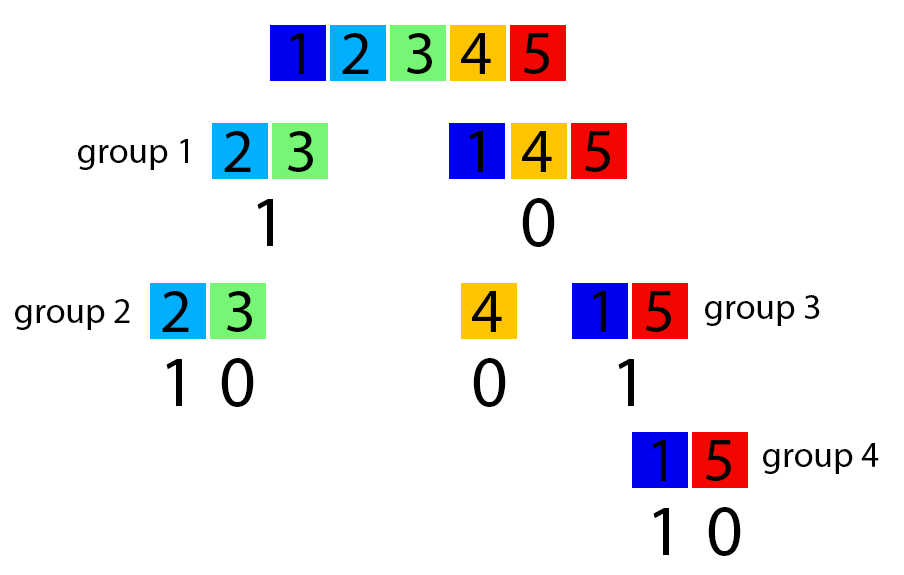
\includegraphics[width=0.6\textwidth]{capitulo_3/imagens/grouping.png}
\end{figure}

Os quatro grupos de amostras gerados com a regra de hierarquia são apresentados na \autoref{fig:jura_mc}. O primeiro grupo contém todas as amostras do conjunto de dados, enquanto os outros são subconjuntos.

\begin{figure}[H]
    \caption{Mapa de localização das amostras dos quatro grupos.} \label{fig:jura_mc}
     \centering
     \subfloat[][Grupo 1]{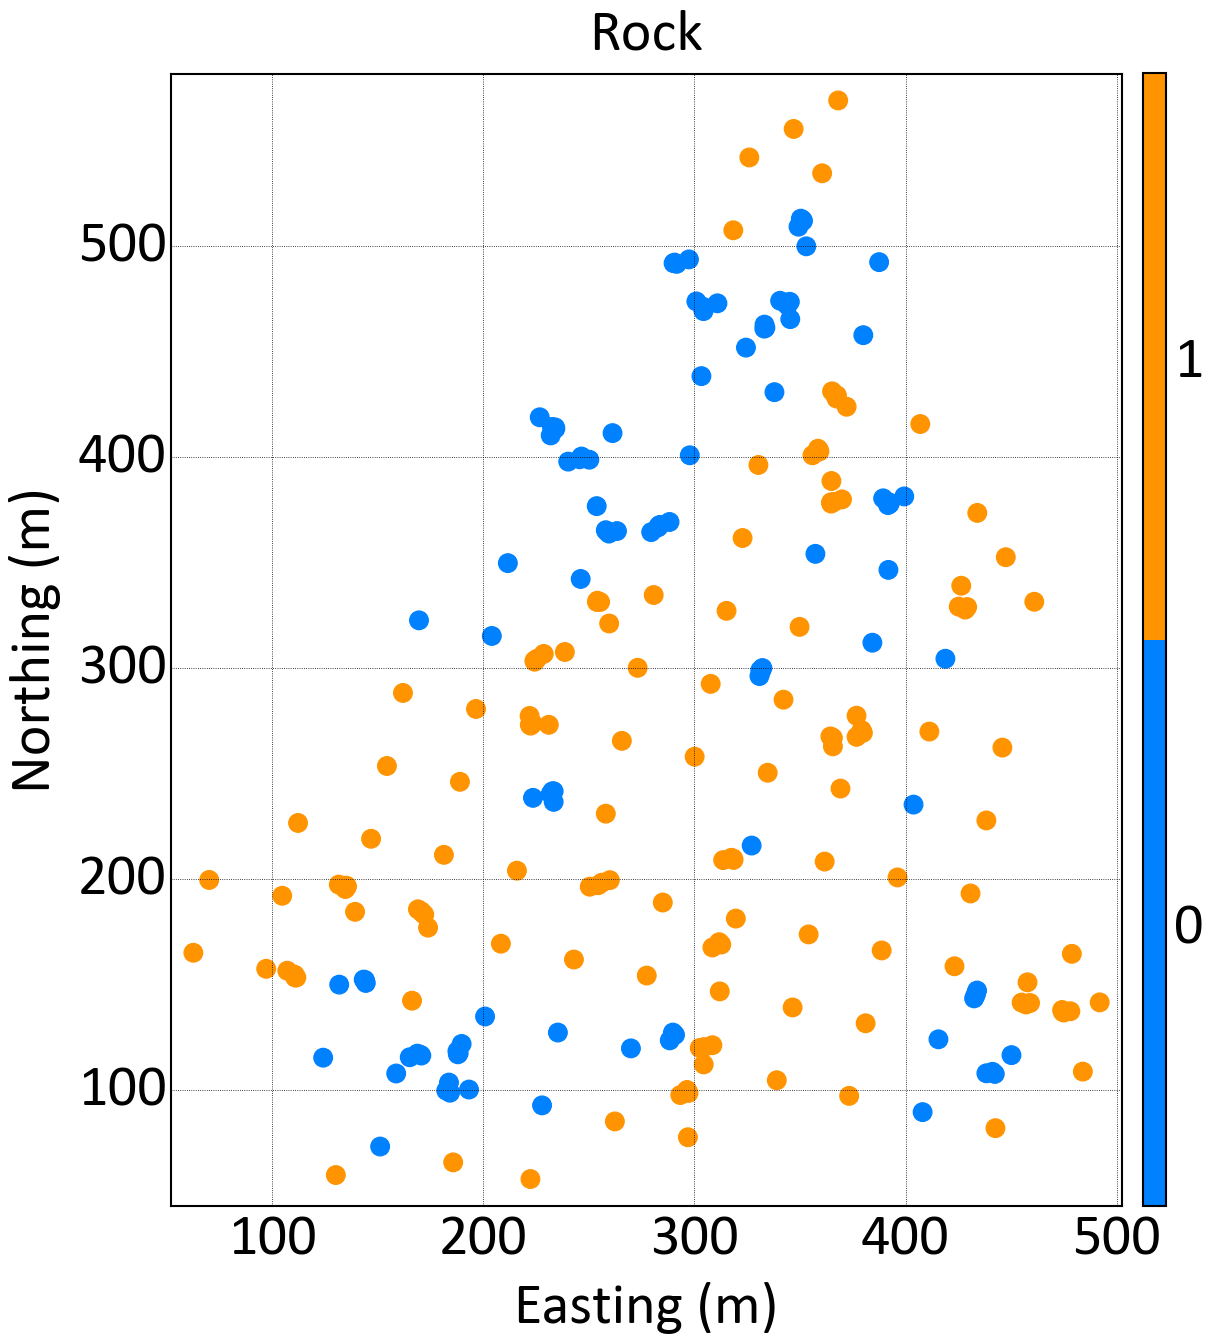
\includegraphics[height=150pt]{capitulo_3/imagens/gg1.png}\label{fig:g1}}
     \hspace{1em}
     \subfloat[][Grupo 2]{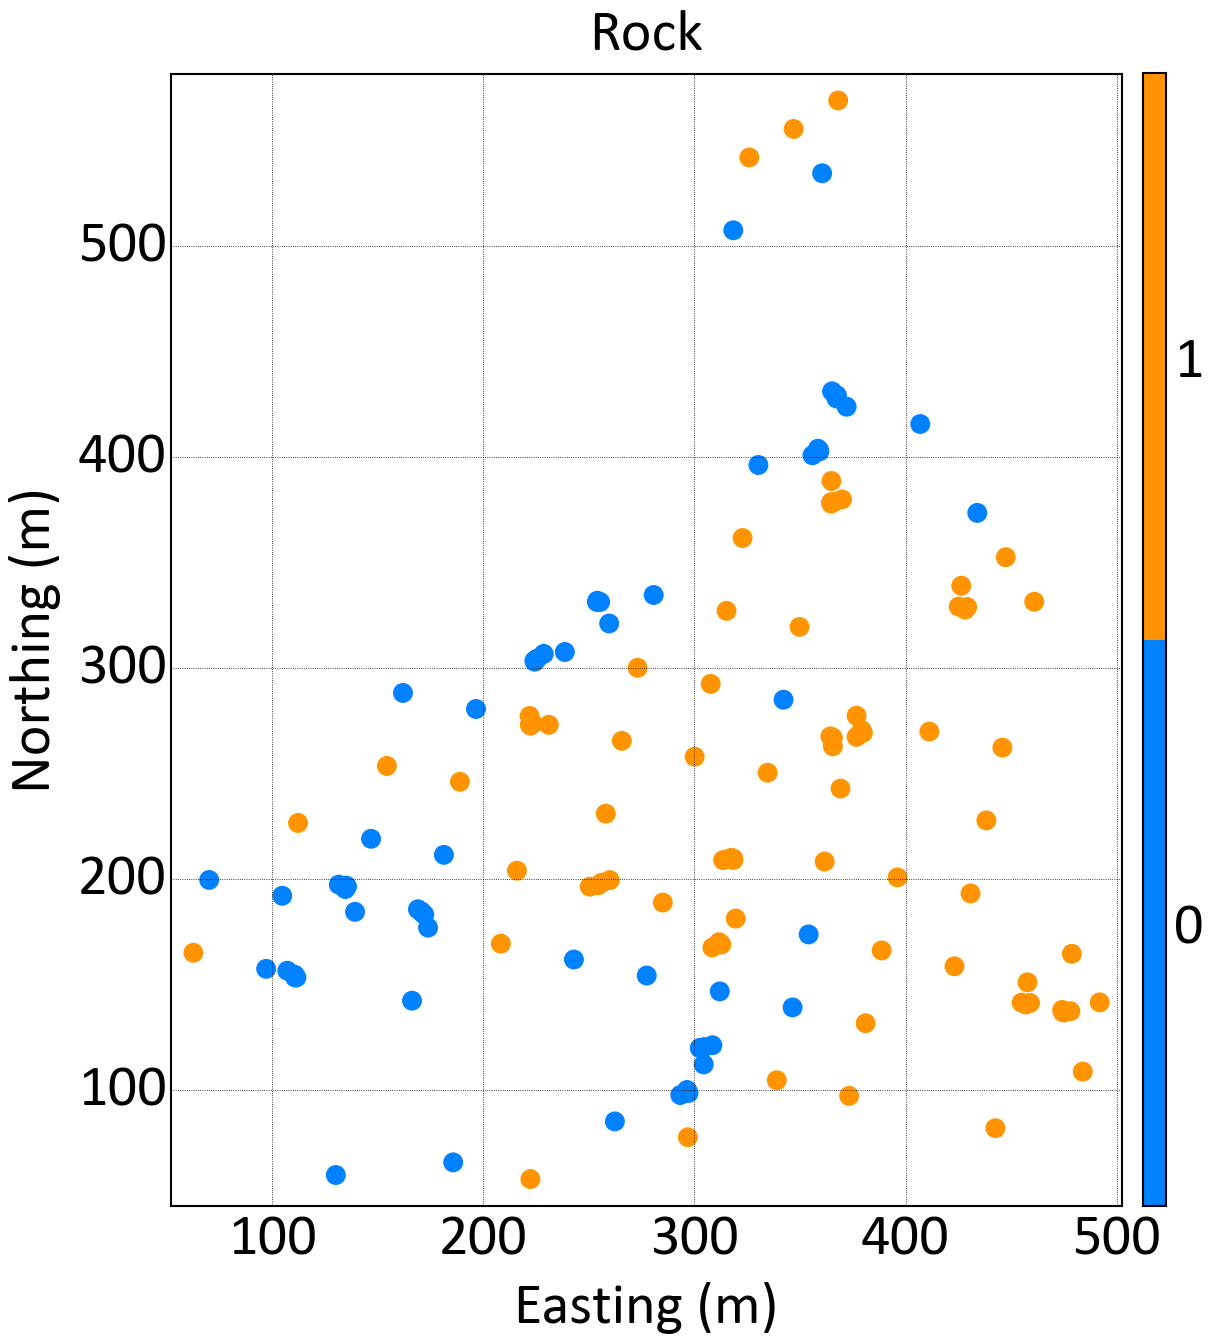
\includegraphics[height=150pt]{capitulo_3/imagens/gg2.png}\label{fig:g2}}\\
     \subfloat[][Grupo 3]{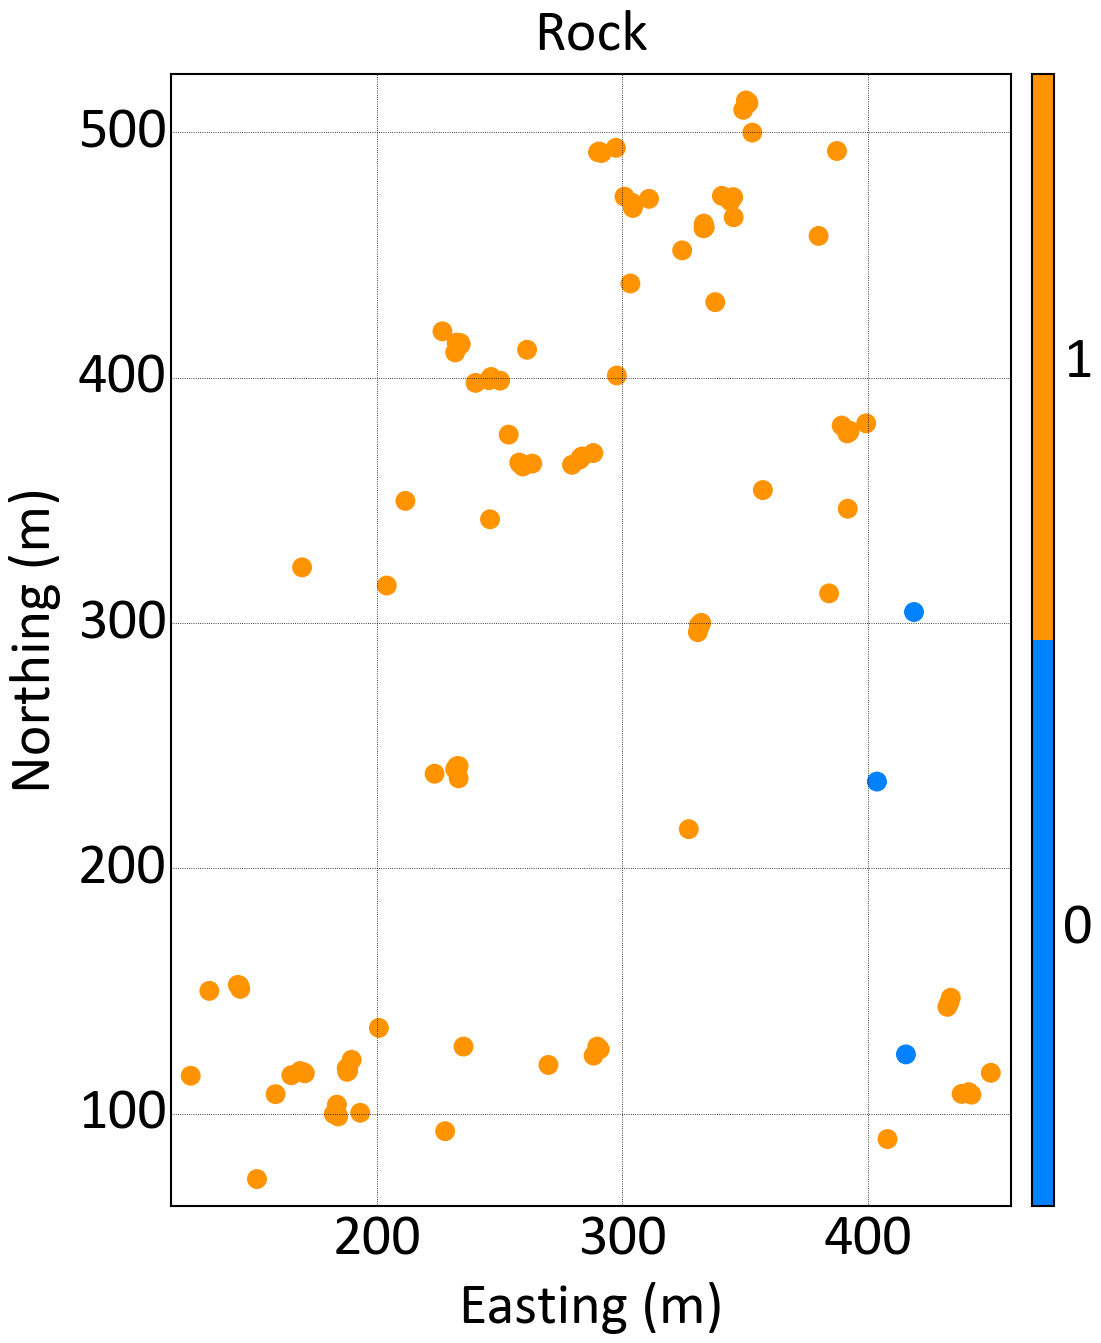
\includegraphics[height=150pt]{capitulo_3/imagens/gg3.png}\label{fig:g3}}
     \hspace{1em}
     \subfloat[][Grupo 4]{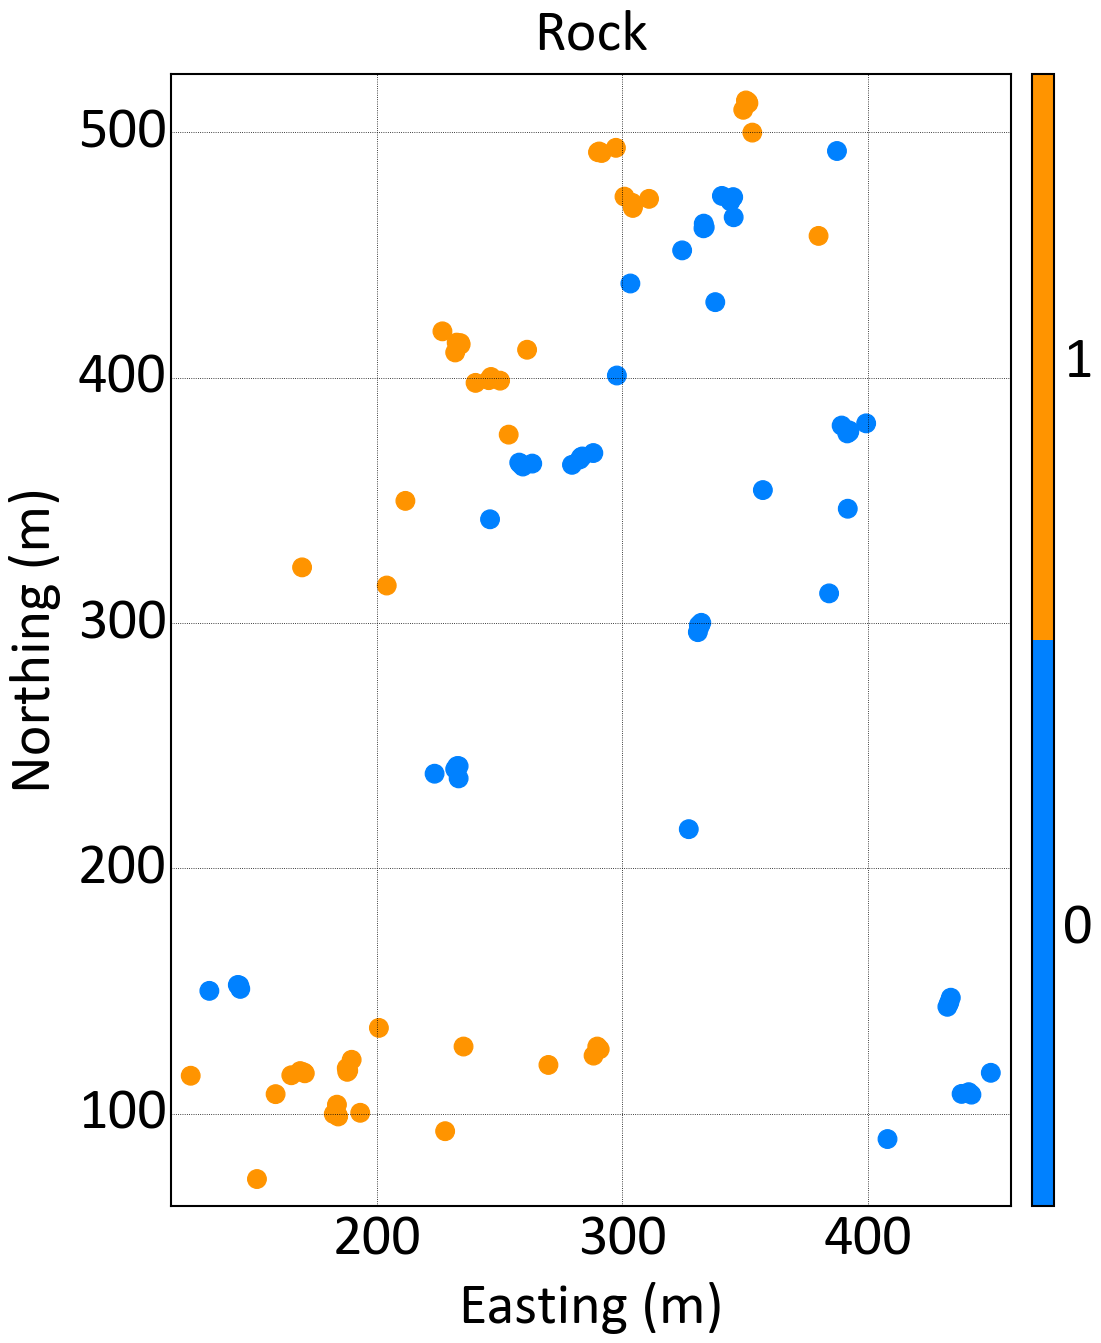
\includegraphics[height=150pt]{capitulo_3/imagens/gg4.png}\label{fig:g4}}
\end{figure}

É necessário definir uma zona de incerteza em torno dos contatos entre os indicadores de cada grupo. Blocos localizados fora da zona são considerados como pertencentes a um determinado indicador, enquanto blocos dentro da zona terão sua incerteza avaliada. A zona de incerteza é obtida usando o mesmo parâmetro C apresentado na \autoref{boundsim} para criar e controlar a espessura/tamanho da zona. O parâmetro C deve ser calibrado ou determinado para cada grupo. Para o exemplo do \textit{Swiss Jura}, um valor C de 12 metros foi escolhido para todos os quatro grupos.

As propriedades funções distância assinaladas devem ser calculadas, modificadas pelo parâmetro C de acordo com a \autoref{C_dist}, e interpoladas para cada grupo. A interpolação estima para cada nó do \textit{grid} o valor da função de distância modificada. A zona de incerteza, para cada grupo, é determinada pelos blocos com valores estimados entre $ -C $ e $ + C $.

A figura \autoref{fig:jura_int} mostra as distâncias assinaladas modificadas interpoladas para cada grupo. A interpolação foi realizada em um \textit{grid} de 3x3 metros por RBF usando \textit{kernels} Gaussianos equivalentes aos variogramas dos indicadores.

\begin{figure}[H]
    \caption{Distâncias modificadas e interpoladas para cada um dos grupos.} \label{fig:jura_int}
     \centering
     \subfloat[][Grupo 1]{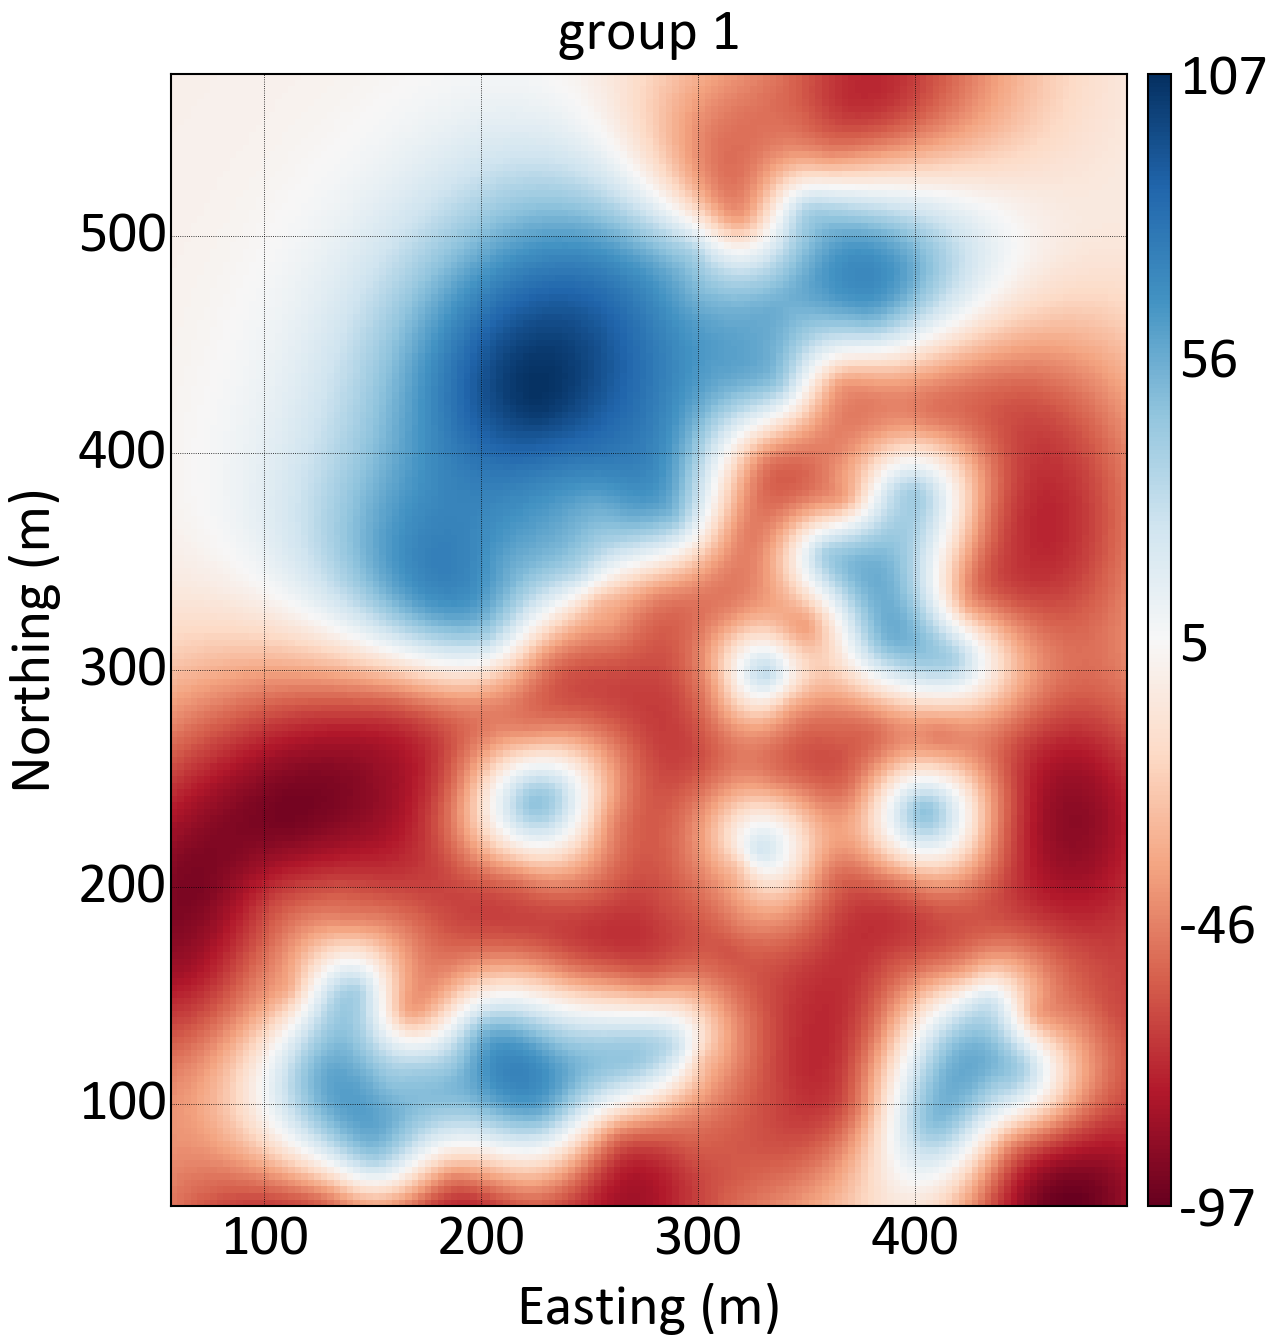
\includegraphics[height=150pt]{capitulo_3/imagens/int_g1.png}\label{fig:int1}}
     \hspace{1em}
     \subfloat[][Grupo 2]{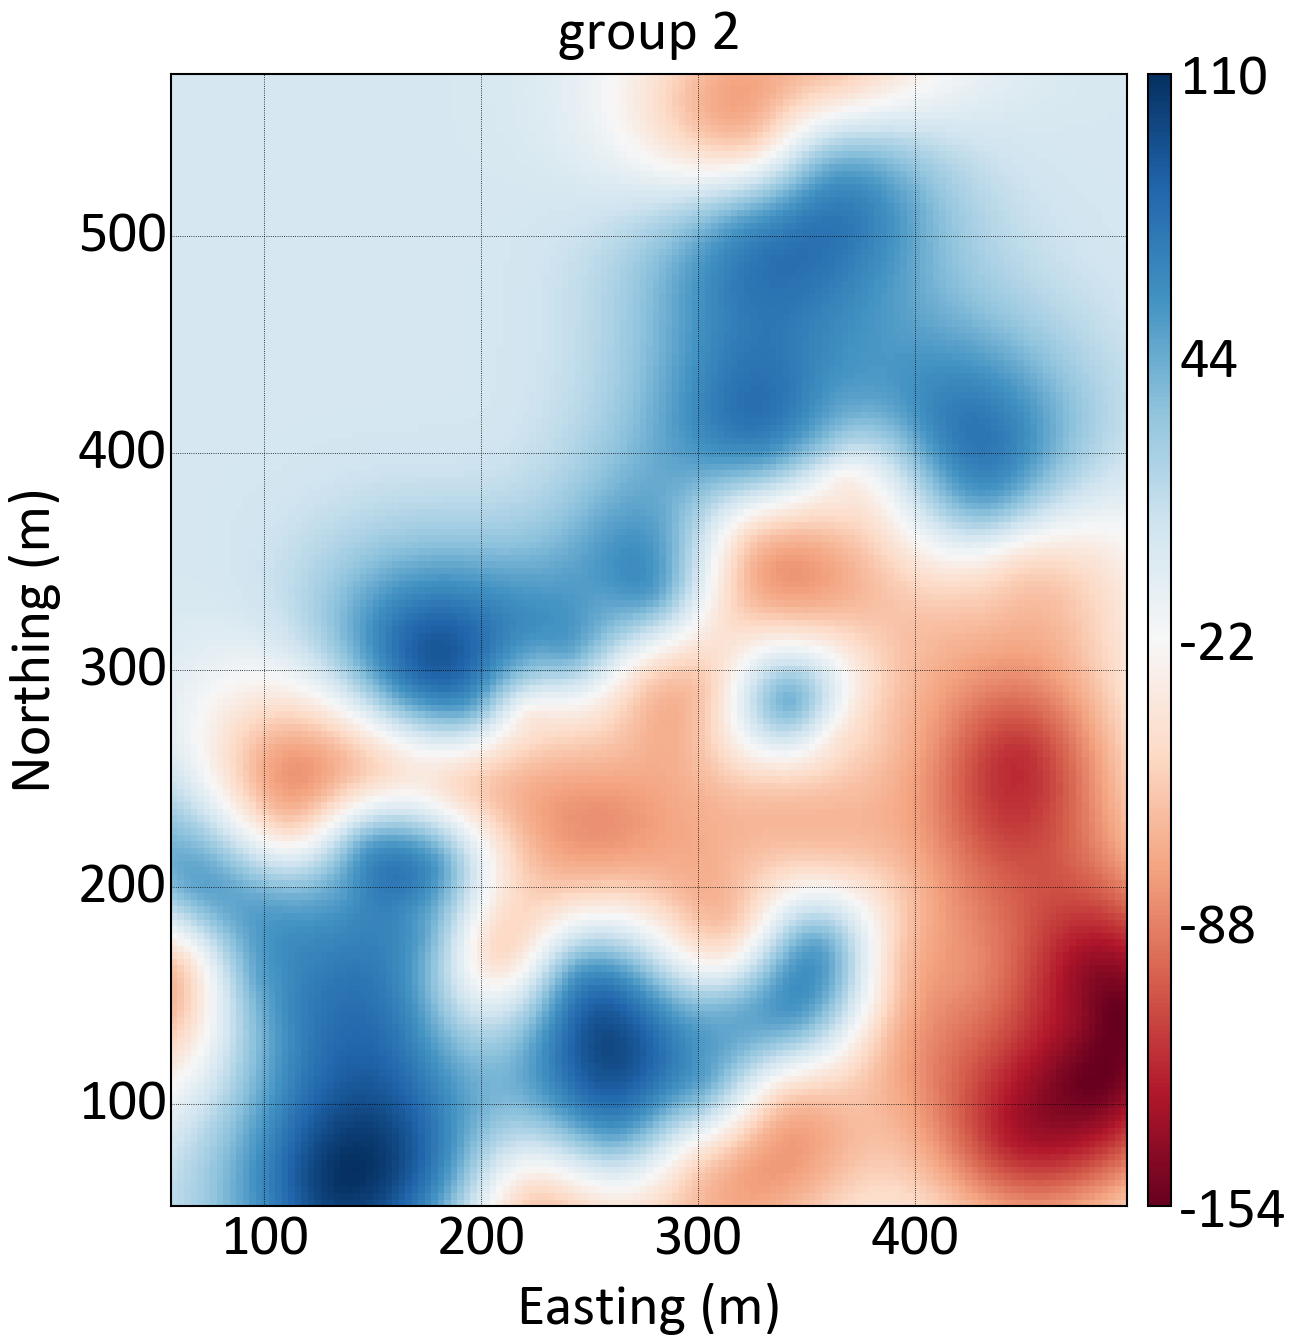
\includegraphics[height=150pt]{capitulo_3/imagens/int_g2.png}\label{fig:int2}}\\
     \subfloat[][Grupo 3]{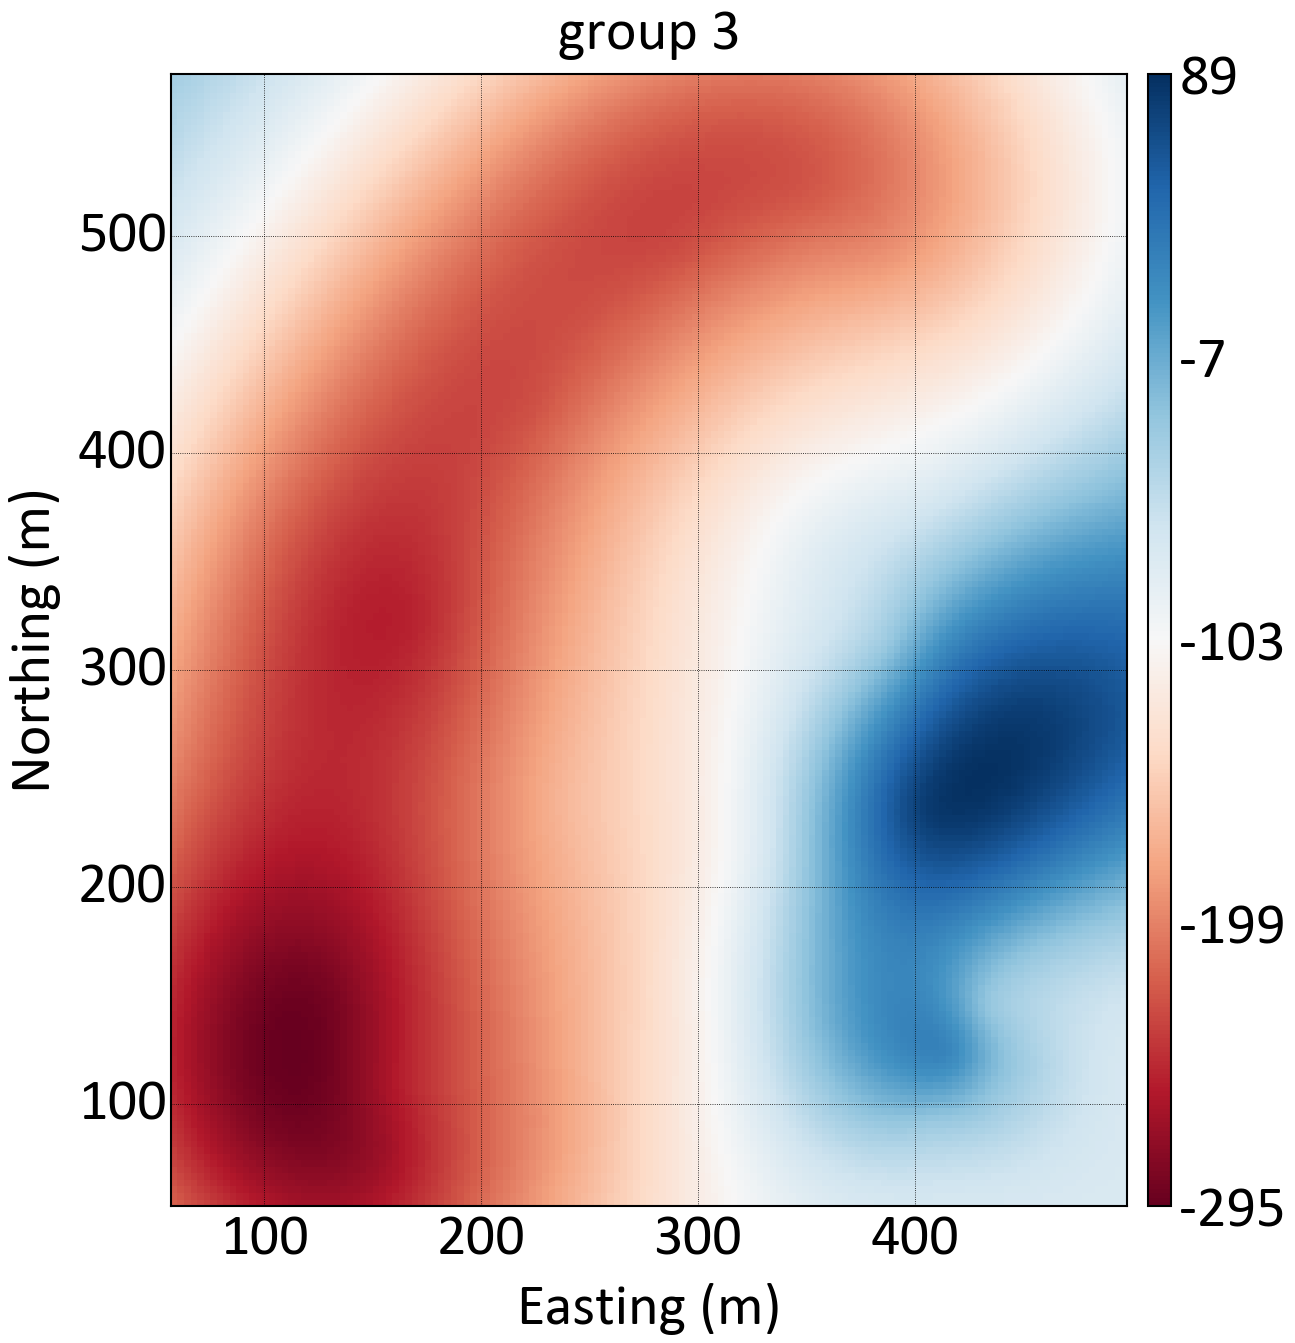
\includegraphics[height=150pt]{capitulo_3/imagens/int_g3.png}\label{fig:int3}}
     \hspace{1em}
     \subfloat[][Grupo 4]{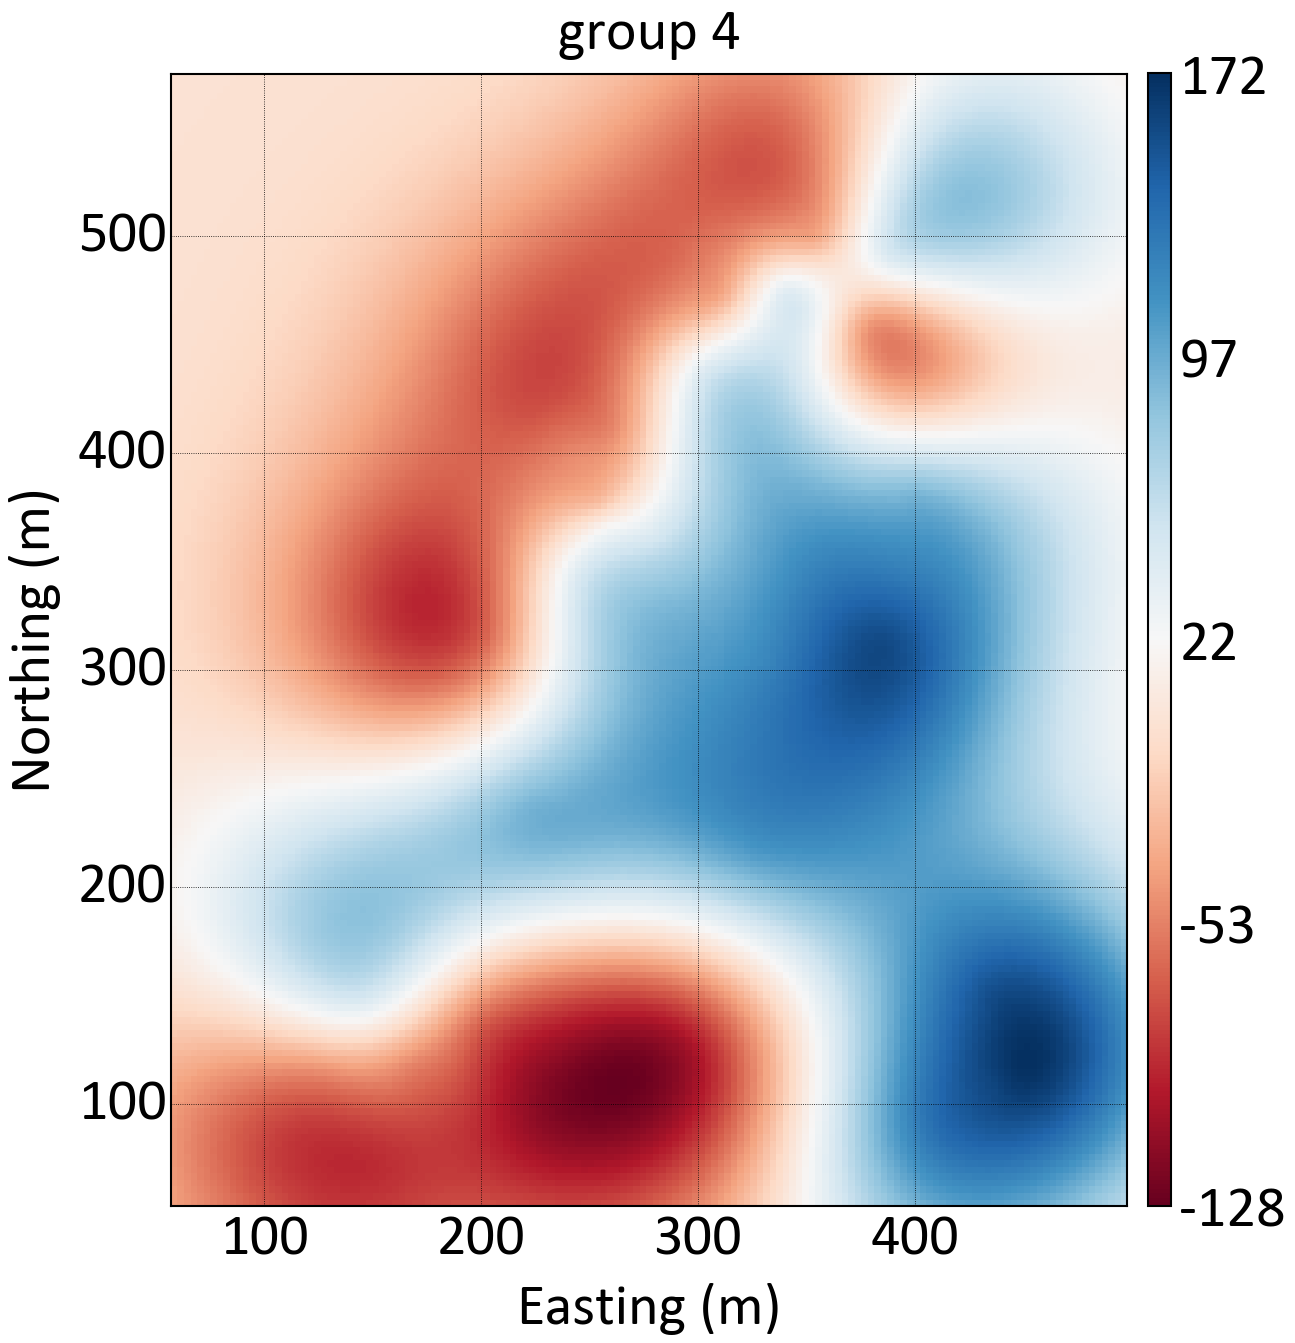
\includegraphics[height=150pt]{capitulo_3/imagens/int_g4.png}\label{fig:int4}}
\end{figure}

A figura \autoref{fig:jura_sim} apresenta, uma realização de um total de 10, dos valores gaussianos simulados dentro da zona de incerteza para cada grupo. A zona de incerteza é definida truncando os valores interpolados da \autoref{fig:jura_int} entre $ -C $ e $ + C $, nesse caso 12 metros.

Como um contato está sendo simulado, é recomendado o uso de um variograma Gaussiano para a simulação não condicional, pois permite que a continuidade de curto alcance seja reproduzida (\cite{wilde2012kriging}). Além disso, é recomendável usar um pequeno efeito pepita para evitar instabilidades de cálculo. O alcance do variograma Gaussiano usado na simulação de $y^l(u)$ determina as características do contato. Alcances menores geram contatos mais ásperos, enquanto alcances maiores geram contatos mais suaves. \citeonline{martin2017implicitmodeling} advoga que o mesmo variograma (ou o seu equivalente) usado para interpolar as distâncias assinaladas pode ser usado para simular os valores Gaussianos.

\begin{figure}[H]
    \caption{Valores Gaussianos simulados, dentro da zona de incerteza, para cada grupo.} \label{fig:jura_sim}
     \centering
     \subfloat[][Valores Gaussianos simulados para o grupo 1.]{\includegraphics[height=150pt]{capitulo_3/imagens/jurareal1.png}\label{fig:int1}}
     \hspace{1em}
     \subfloat[][Valores Gaussianos simulados para o grupo 2.]{\includegraphics[height=150pt]{capitulo_3/imagens/jurareal2.png}\label{fig:int2}}\\
     \subfloat[][Valores Gaussianos simulados para o grupo 3.]{\includegraphics[height=150pt]{capitulo_3/imagens/jurareal3.png}\label{fig:int3}}
     \hspace{1em}
     \subfloat[][Valores Gaussianos simulados para o grupo 4.]{\includegraphics[height=150pt]{capitulo_3/imagens/jurareal4.png}\label{fig:int4}}
\end{figure}

\subsection{Estudo de caso}

\subsection{Discussão}